%%%%%%%%%%%%%%%%%%%%%%%%%%%
% PREAMBOLO DEL DOCUMENTO %
%%%%%%%%%%%%%%%%%%%%%%%%%%%
\documentclass[a4paper,11pt,oneside,top=3cm,bottom=3cm,left=0cm,right=0cm,openright,reqno,table]{book}

% openany - fa iniziare i capitoli direttamente nella pagina successiva
% openright - fa iniziare i capitoli nella prima pagina destra disponibile 
% fleqn  - allinea le formule a sinistra anzichè centrarle
% leqno - dispone la numerazione delle formule sulla sinistra o destra
% reqno - dispone la numerazione delle formule sulla destra
%
\usepackage{packages}
% Per non appesantire troppo questo file
% quasi tutti i pacchetti usati sono salvati in packages.sty
%
\linespread{1.5}

% Per avere la parola BOZZA scritta su tutte le pagine

% funziona solo in modalità PS
% Invece per i PDF ho risolto così:
% pdftk tesi.pdf background bozza.pdf output tesi_bozza.pdf
%
%%%%%%%%%%%%%%%%%%%%%%%%%%%%%%%%%
%   DOCUMENTO VERO E PROPRIO    %
%%%%%%%%%%%%%%%%%%%%%%%%%%%%%%%%%
\begin{document}
% FRONTESPIZIO %
\begin{titlepage}
\changepage{}{}{}{}{}{}{}{}{}
% parametri per cambiare le dimensioni di una singola pagina in ordine:
% {textheight}{textwidth}{evensidemargin}{oddsidemargin}{columnsep}
% {topmargin}{headheight}{headsep}{footskip}
% se voglio centrare la pagina devo mettere bindingoffset/2
% i primi 5 parametri posso usarli con \changetext


\begin{center}

\includegraphics [width=.15\columnwidth, angle=0]{capitoli/images/unisa.pdf}\\ % height
\vspace{0.5cm}
{\LARGE \scshape Università degli Studi di Salerno}\\
\vspace{1cm}
{\Large Dipartimento di Informatica}\\
\vspace{2cm}
{\Large \scshape Statistica e Analisi dei Dati} \\
\vspace{2cm}
{\huge \bfseries Inferenza Statistica Distribuzione Normale} \\
\vspace{6cm}

\begin{minipage}[t]{7cm}
\flushleft
\textsc{Docente}

Prof.ssa \textbf{Amelia G. Nobile} \\[0.25cm]

\end{minipage}
\hfill
\begin{minipage}[t]{7cm}
\flushright
\textsc{Candidato}

\textbf{Mattia Mori} \\
Matricola: 0512105707
\end{minipage}

\vspace{2cm}

%& & \\
%& Candidato & \\
%& \textbf{Mattia Mori} & \\
{\small Anno Accademico 2022-2023} %\\

\end{center}

\end{titlepage}
\setlength{\headheight}{14pt}

\frontmatter
% quello che segue è in numerazione romana e i capitoli non verranno numerati
% se non si vuole che compaia il numero di pagina basta usare il comando:
%\nonumber

% RINGRAZIAMENTI %
\include{frontmatter/ringraziamenti}
% SOMMARIO %
\cleardoublepage
\include{frontmatter/sommario}
% INDICI %
\phantomsection
\addcontentsline{toc}{chapter}{Indice}
\tableofcontents
% Il simbolo * serve per evitare che comapaia nell'indice
\clearpage
%\listoffigures
%\clearpage
%\listoftables
% GLOSSARIO
%\cleardoublepage
\phantomsection
\addcontentsline{toc}{chapter}{Glossario}
% per inserire l'elenco dei simboli e degli acronimi nell'indice
\printglossary
% Per stampare il glossario
% per aggiornarlo si deve eseguire da terminale:
% makeindex -s myDoc.ist -t myDoc.alg -o myDoc.acr myDoc.acn
% per inserire una voce nell'elenco:
% \newglossaryentry{voce_etichetta}{name={voce}, description={descrizione}}
% se non compare direttamente nel testo va inizializzata con:
% \glsadd{voce_etichetta}
% oppure se viene richiamata all'interno del testo:
% \gls{voce_etichetta}
% SIMBOLI E NOTAZIONI %
%%%%%%%%%%%%%%%%%%%%%%%%%%%%%%%\cleardoublepage
\phantomsection
\addcontentsline{toc}{chapter}{Elenco delle tabelle}
% per inserire l'elenco dei simboli e degli acronimi nell'indice
%\printglossary[type=\acronymtype,title=Elenco delle figure]
% Per stampare l'elenco dei simboli
\listoftables
% per aggiornarlo si deve eseguire da terminale:
% makeindex -s myDoc.ist -t myDoc.glg -o myDoc.gls myDoc.glo
% per inserire una voce nell'elenco:
% \newglossaryentry{voce_etichetta}{name={voce}, description={descrizione}}
% se non compare direttamente nel testo va inizializzata con:
% \glsadd{voce_etichetta}
% oppure se viene richiamata all'interno del testo:
% \gls{voce_etichetta}

\mainmatter
% quello che segue sarà in numerazione araba e i capitoli verranno numerati
%\part{Studio iniziale}
% CAPITOLI
\phantomsection
\definecolor{dkgreen}{rgb}{0,0.6,0}
\definecolor{gray}{rgb}{0.5,0.5,0.5}
\definecolor{mauve}{rgb}{0.58,0,0.82}


\lstset{frame=tb,
language=R,
aboveskip=3mm,
belowskip=3mm,
showstringspaces=false,
columns=flexible,
numbers=none,
inputencoding=utf8/latin1,
keywordstyle=\color{blue},
numberstyle=\tiny\color{gray},
commentstyle=\color{dkgreen},
stringstyle=\color{mauve},
breaklines=true,
breakatwhitespace=true,
tabsize=3
}


\chapter{Introduzione}\label{cap1}

In ogni età e fase della vita, svolgere attività fisica con regolarità significa fare una scelta a favore della propria salute: praticata regolarmente, l’attività fisica contribuisce a mantenere e migliorare il benessere psicofisico, a ridurre i sintomi di ansia, stress, depressione e solitudine, perché può essere svolta in compagnia, migliora il sonno, aiuta a smettere di fumare. Aiuta la riduzione della pressione arteriosa e il controllo del livello di glicemia e colesterolo nel sangue, aiuta a prevenire malattie metaboliche, cardiovascolari e neoplastiche e artrosi e contribuisce a ridurre il tessuto adiposo in eccesso perché facilita il raggiungimento del bilancio energetico. Comporta benefici evidenti anche per l’apparato muscolo-scheletrico e riduce il rischio di cadute nella popolazione anziana. Contribuisce, inoltre, a gestire le principali patologie croniche non trasmissibili e quindi a migliorare la qualità della vita. Andremo a studiare e commentare con questo lavoro le abitudini sportive delle persone all'interno delle regioni.
Di seguito, viene definito il dataset impiegato.

\section{Dataset}\label{cap1.1}

I dati che compongono il dataset sono stati recuperati dal sito web dell'\textbf{ISTAT} (Istituto Nazionale di Statistica). 

Il dataset si presenta come una tabella dove:
\begin{itemize}
  \item Le righe rappresentano le regioni italiane
  \item Le colonne indicano quanta attività fisica svolge una persona
\end{itemize}

I dati che compongono il dataset si riferiscono a un'indagine condotta nell'anno 2021. Inoltre, i dati raccolti sono delle stime riportate su un campione di 100 persone con le stesse caratteristiche dai 3 anni in su.

Di seguito, la tabella con i dati relativi:

\begin{figure}[!htb]
    \centering
    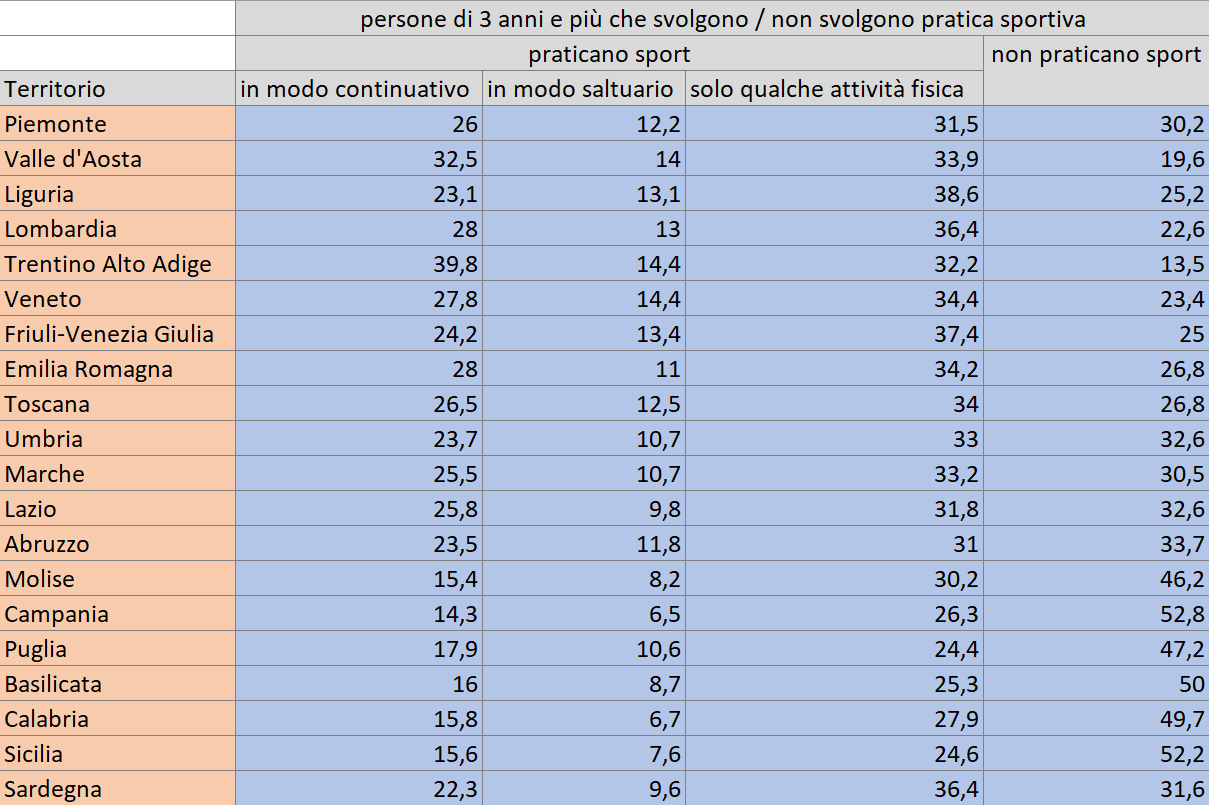
\includegraphics[height=11cm]{ProgettoSAD/capitoli/images/dataset_image.png}
    \caption{Dataset di riferimento.}
    \captionsetup{font={footnotesize,bf,it}}
    \label{fig:dataset_image}
\end{figure}

Al fine di poter lavorare in R sul dataset esportato, esso viene inserito all'interno di un \textbf{dataframe}.

\vspace{5mm}
\begin{lstlisting}
regioni <- c("Piemonte", "ValleD'Aosta", "Liguria", "Lombardia", "TrentinoAltoAdige",
             "Veneto", "Friuli-VeneziaGiulia", "Emilia-Romagna", "Toscana", "Umbria",
             "Marche", "Lazio", "Abruzzo", "Molise", "Campania", "Puglia",
             "Basilicata", "Calabria", "Sicilia", "Sardegna")


df <- data.frame(Modo.Cont. =
                   c(26, 32.5, 23.1, 28, 39.8, 27.8, 24.2, 28, 26.5, 23.7, 25.5,
                     25.8, 23.5, 15.4, 14.3, 17.9, 16, 15.8, 15.6, 22.3),
                 Modo.Salt. =
                   c(12.2, 14, 13.1, 13, 14.4, 14.4, 13.4, 11, 12.5, 10.7,
                     10.7, 9.8, 11.8, 8.2, 6.5, 10.6, 8.7, 6.7, 7.6, 9.6),
                 Qualche.Att. =
                   c(31.5, 33.9, 38.6, 36.4, 32.2, 34.4, 37.4, 34.2, 34, 33,
                     33.2, 31.8, 31, 30.2, 26.3, 24.4, 25.3, 27.9, 24.6, 36.4),
                 Non.Prat.Sport. =
                   c(30.2, 19.6, 25.2, 22.6, 13.5, 23.4, 25, 26.8, 26.8, 32.6,
                     30.5, 32.6, 33.7, 46.2, 52.8, 47.2, 50, 49.7, 52.2, 31.6))
row.names(df) <- regioni
\end{lstlisting}
\vspace{5mm}

Attraverso la funzione \textit{data.frame()} si è organizzato il dataset in righe e 
colonne. In particolare le colonne sono state costituite come vettori di valori 
numerici tramite la funzione di concatenazione \textit{c()}, attribuendo a ciascuna 
colonna il nome della relativa caratteristica. Successivamente le righe del 
dataframe sono state rinominate con i nomi delle regioni italiane attraverso 
la funzione \textit{row.names(dataset)}.



%################################################

\newpage
\phantomsection
\definecolor{dkgreen}{rgb}{0,0.6,0}
\definecolor{gray}{rgb}{0.5,0.5,0.5}
\definecolor{mauve}{rgb}{0.58,0,0.82}


\lstset{frame=tb,
language=R,
aboveskip=3mm,
belowskip=3mm,
showstringspaces=false,
columns=flexible,
numbers=none,
inputencoding=utf8/latin1,
keywordstyle=\color{blue},
numberstyle=\tiny\color{gray},
commentstyle=\color{dkgreen},
stringstyle=\color{mauve},
breaklines=true,
breakatwhitespace=true,
tabsize=3
}

\chapter{Grafici}\label{cap2} %\label{1cap:spinta_laterale}

In questo capitolo verranno mostrati \textbf{grafici a barre} e \textbf{grafici a torta} per rappresentare i dati del dataset, evidenziandone le principali caratteristiche.

Il dataset sarà analizzato con grafici sia in base alle singole regioni, sia in base alle singole caratteristiche.

\section{Grafici a barre: Caratteristiche}\label{cap2.1}

In questa sezione verrà mostrato un grafico a barre per ogni caratteristica del dataset, al fine di poter confrontare tra le varie regioni le abitudini principali delle persone; inoltre, ogni grafico sarà correlato con la propria media campionaria.

\vspace{5mm}
\noindent \textbf{Costruzione del grafico a barre}

Per la costruzione di un grafico a barre si utilizzano le seguenti linee di codice:

\vspace{5mm}
\begin{lstlisting}
  bp1 <- barplot(df$Modo.Cont., main = "Persone che praticano sport in modo continuativo nelle regioni", col = rainbow(20))
  abline(h = mean(df$Modo.Cont.), lty = 2, col = "red")
  text(bp1, par("usr")[3], labels = row.names(df), srt = 45, adj = c(1, 1), xpd = TRUE, cex = 0.8)

  bp1 <- barplot(df$Modo.Salt., main = "Persone che praticano sport in modo saltuario nelle regioni", col = rainbow(20))
  abline(h = mean(df$Modo.Salt.), lty = 2, col = "red")
  text(bp1, par("usr")[3], labels = row.names(df), srt = 45, adj = c(1, 1), xpd = TRUE, cex = 0.8)

  bp1 <- barplot(df$Qualche.Att., main = "Persone che praticano solo qualche attività fisica nelle regioni", col = rainbow(20))
  abline(h = mean(df$Qualche.Att.), lty = 2, col = "red")
  text(bp1, par("usr")[3], labels = row.names(df), srt = 45, adj = c(1, 1), xpd = TRUE, cex = 0.8)

  bp1 <- barplot(df$Non.Prat.Sport., main = "Persone che non praticano sport nelle regioni", col = rainbow(20))
  abline(h = mean(df$Non.Prat.Sport.), lty = 2, col = "red")
  text(bp1, par("usr")[3], labels = row.names(df), srt = 45, adj = c(1, 1), xpd = TRUE, cex = 0.8)

\end{lstlisting}
\vspace{5mm}

Dove la variabile \textit{bp1} memorizza un barplot relativo alla frequenza delle attività sportive nelle varie regioni. I dati del dataset sono recuperati attraverso \textit{df\$Modo.Cont.}, mentre ulteriori caratteristiche associate al grafico, come il titolo e i colori da utilizzare per le barre sono gestite rispettivamente dai parametri \textit{main} e \textit{col}. Per evidenziare, invece, la media di tale caratteristica sul grafico è stata aggiunta una retta attraverso la funzione \textit{abline()}. Infine, tramite la funzione \textit{text()}, sono stati aggiunti i nomi delle regioni italiane sull’asse x, ponendoli in modo tale da essere visualizzati per intero.

Di seguito per ciascuna caratteristica il grafico a barre viene costruito con il medesimo codice sopra descritto, sostituendo soltanto il parametro \textit{df\$Modo.Cont.}. con quello della caratteristica presa in osservazione.

\begin{figure}[!htbp]
    \centering
    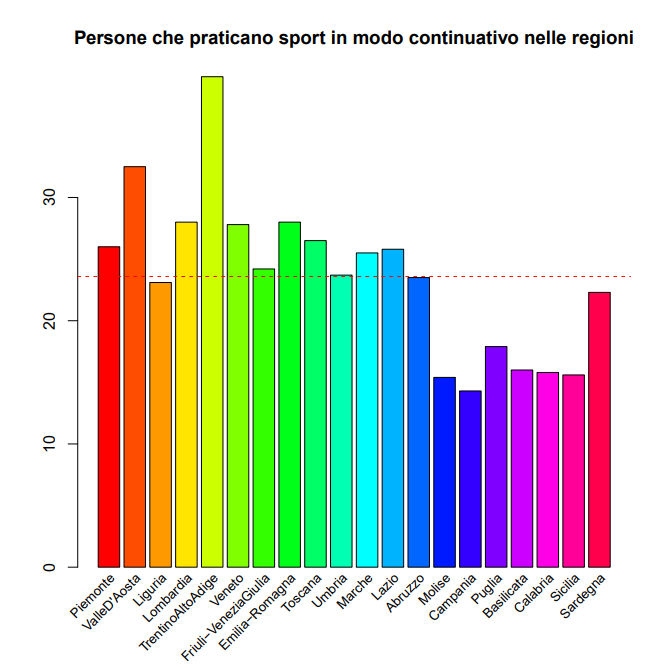
\includegraphics[height=15cm]{ProgettoSAD/capitoli/images/barre_modocont.png}
    \captionsetup{font={footnotesize,bf,it}}
    \label{fig:barre_modocont}
\end{figure}

Si può notare dal grafico che, per quanto riguarda le persone che svolgono attività fisica in modo continuativo, più della metà delle regioni superano la media campionaria, principalmente nel Nord e nel Centro dell'Italia. Il picco più alto è presente nel Trentino Alto Adige, mentre il più basso in Campania.

\begin{figure}[!htbp]
    \centering
    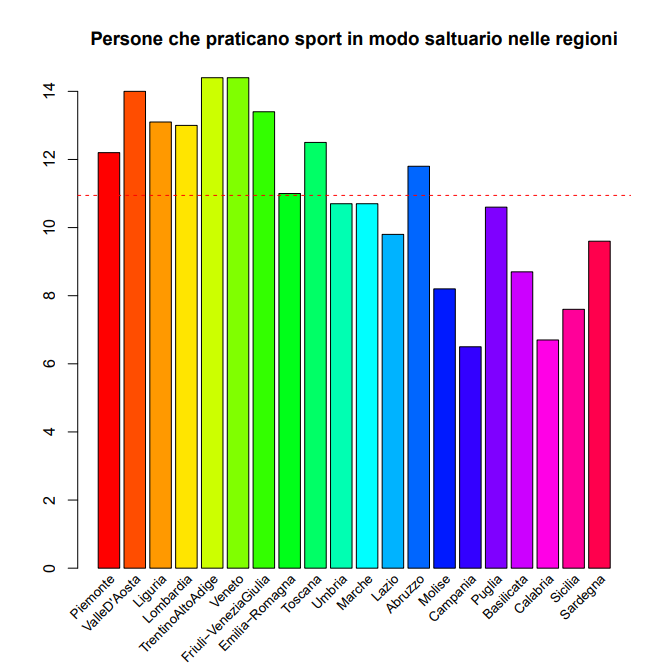
\includegraphics[height=15cm]{ProgettoSAD/capitoli/images/barre_modosalt.png}
    \captionsetup{font={footnotesize,bf,it}}
    \label{fig:barre_modosalt}
\end{figure}

Si può notare dal grafico che, per quanto riguarda le persone che svolgono attività fisica in modo saltuario, meno della metà delle regioni superano la media campionaria, principalmente nel Nord e nel Centro dell'Italia. Si evidenzia che il picco più alto è presente nel Trentino Alto Adige e nel Veneto a parità di persone, mentre il più basso in Campania.

\begin{figure}[!htbp]
    \centering
    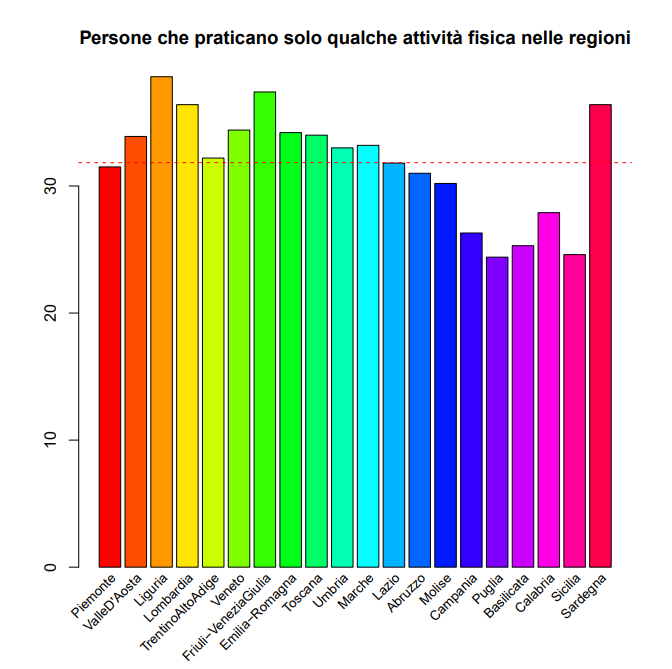
\includegraphics[height=15cm]{ProgettoSAD/capitoli/images/barre_qualcheatt.png}
    \captionsetup{font={footnotesize,bf,it}}
    \label{fig:barre_qualcheatt}
\end{figure}

Si può notare dal grafico che, per quanto riguarda le persone che svolgono qualche attività fisica, meno della metà delle regioni superano la media campionaria, principalmente nel Nord e Centro Italia e la Sardegna. Si evidenzia che il picco più alto è presente in Liguria, mentre il più basso in Puglia.

\begin{figure}[!htbp]
    \centering
    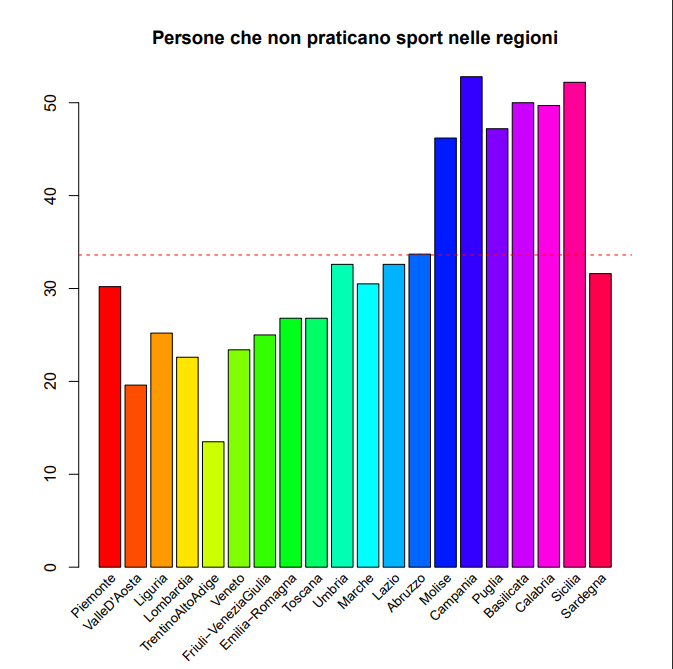
\includegraphics[height=15cm]{ProgettoSAD/capitoli/images/barre_nonpratsport.png}
    \captionsetup{font={footnotesize,bf,it}}
    \label{fig:barre_nonpratsport}
\end{figure}

Si può notare dal grafico che, per quanto riguarda le persone che non svolgono attività sportiva nelle regioni, la media campionaria viene superata da sei regioni, tutte del Sud Italia con la Sicilia. Il picco più alto è registrato in Campania, mentre il più basso in Trentino.

\section{Grafici a barre: Regioni}\label{cap2.2}

In questa sezione verrà mostrato un grafico a barre per ogni regione del dataset al fine di poter confrontare in ognuna di esse la frequenza di attività fisica tra le persone.

Per recuperare le informazioni di ogni singola regione si devono individuare le righe del dataset. Viene creata dunque una funzione per estrarre delle righe in maniera diretta.

Passando in input alla funzione \textit{estraiRiga()} l'indice di riga i e il dataframe, la funzione ritornerà i dati relativi alla i-esima riga del dataset memorizzati in un vettore.

\vspace{5mm}
\begin{lstlisting}
estraiRiga <- function(df, index) {
  vect <- c()
  for (i in df[index,]) {
    vect <- c(vect, i)
  }
  vect
}
\end{lstlisting}
\vspace{5mm}

\noindent \textbf{Costruzione Grafico a barre}

Utilizzando la funzione appena mostrata si è in grado di creare i grafici a barre per le caratteristiche.

\vspace{5mm}
\begin{lstlisting}
  index <- 1
  for (element in regioni) {
    bp1 <- barplot(estraiRiga(df, index),
                   main = element,
                   col = rainbow(4))
    abline(h = mean(estraiRiga(df, index)),
           lty = 2, col = "red")
    text(bp1, par("usr")[3],
         labels = names(df),
         srt = 45,
         adj = c(1.1, 1.1),
         xpd = TRUE, cex = 0.7)
    index <- index + 1
\end{lstlisting}
\vspace{5mm}

\begin{figure}[!htbp]
    \centering
        \subfloat{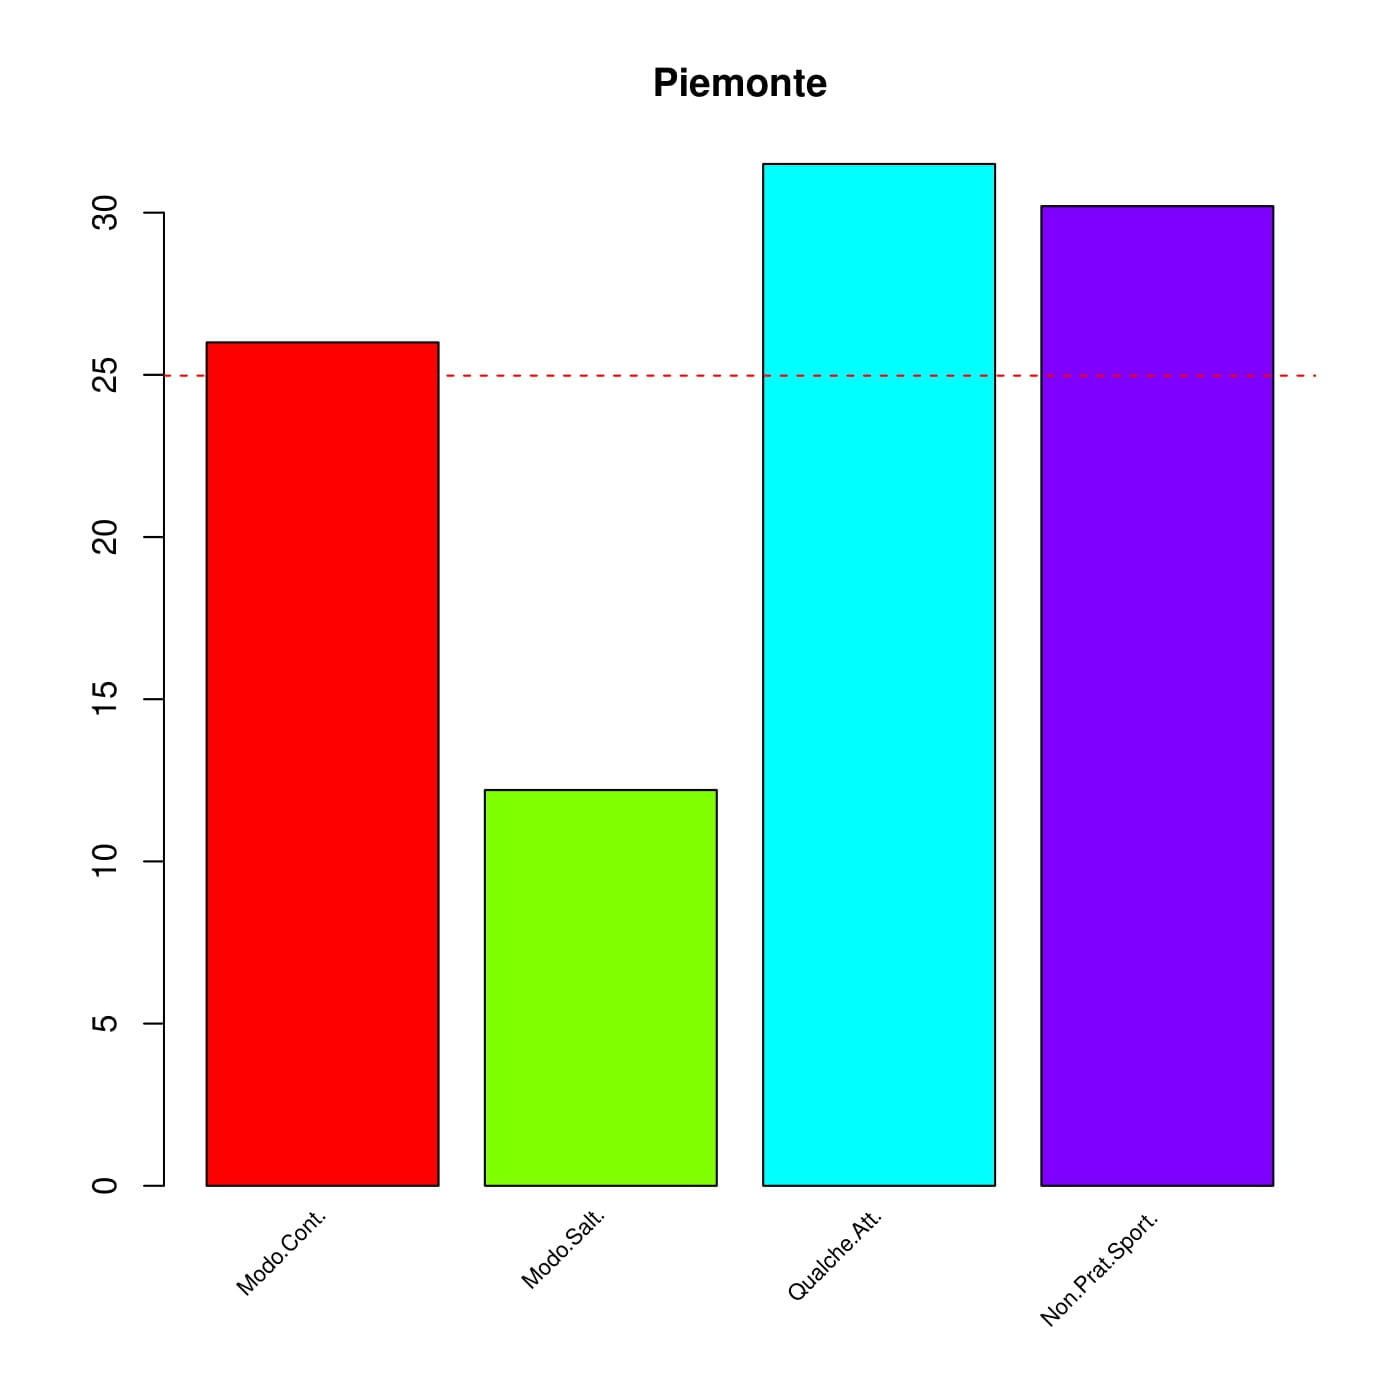
\includegraphics[height=8cm]{ProgettoSAD/capitoli/images/barre_regioni/barre_piemonte.jpg}}
        \qquad
        \subfloat{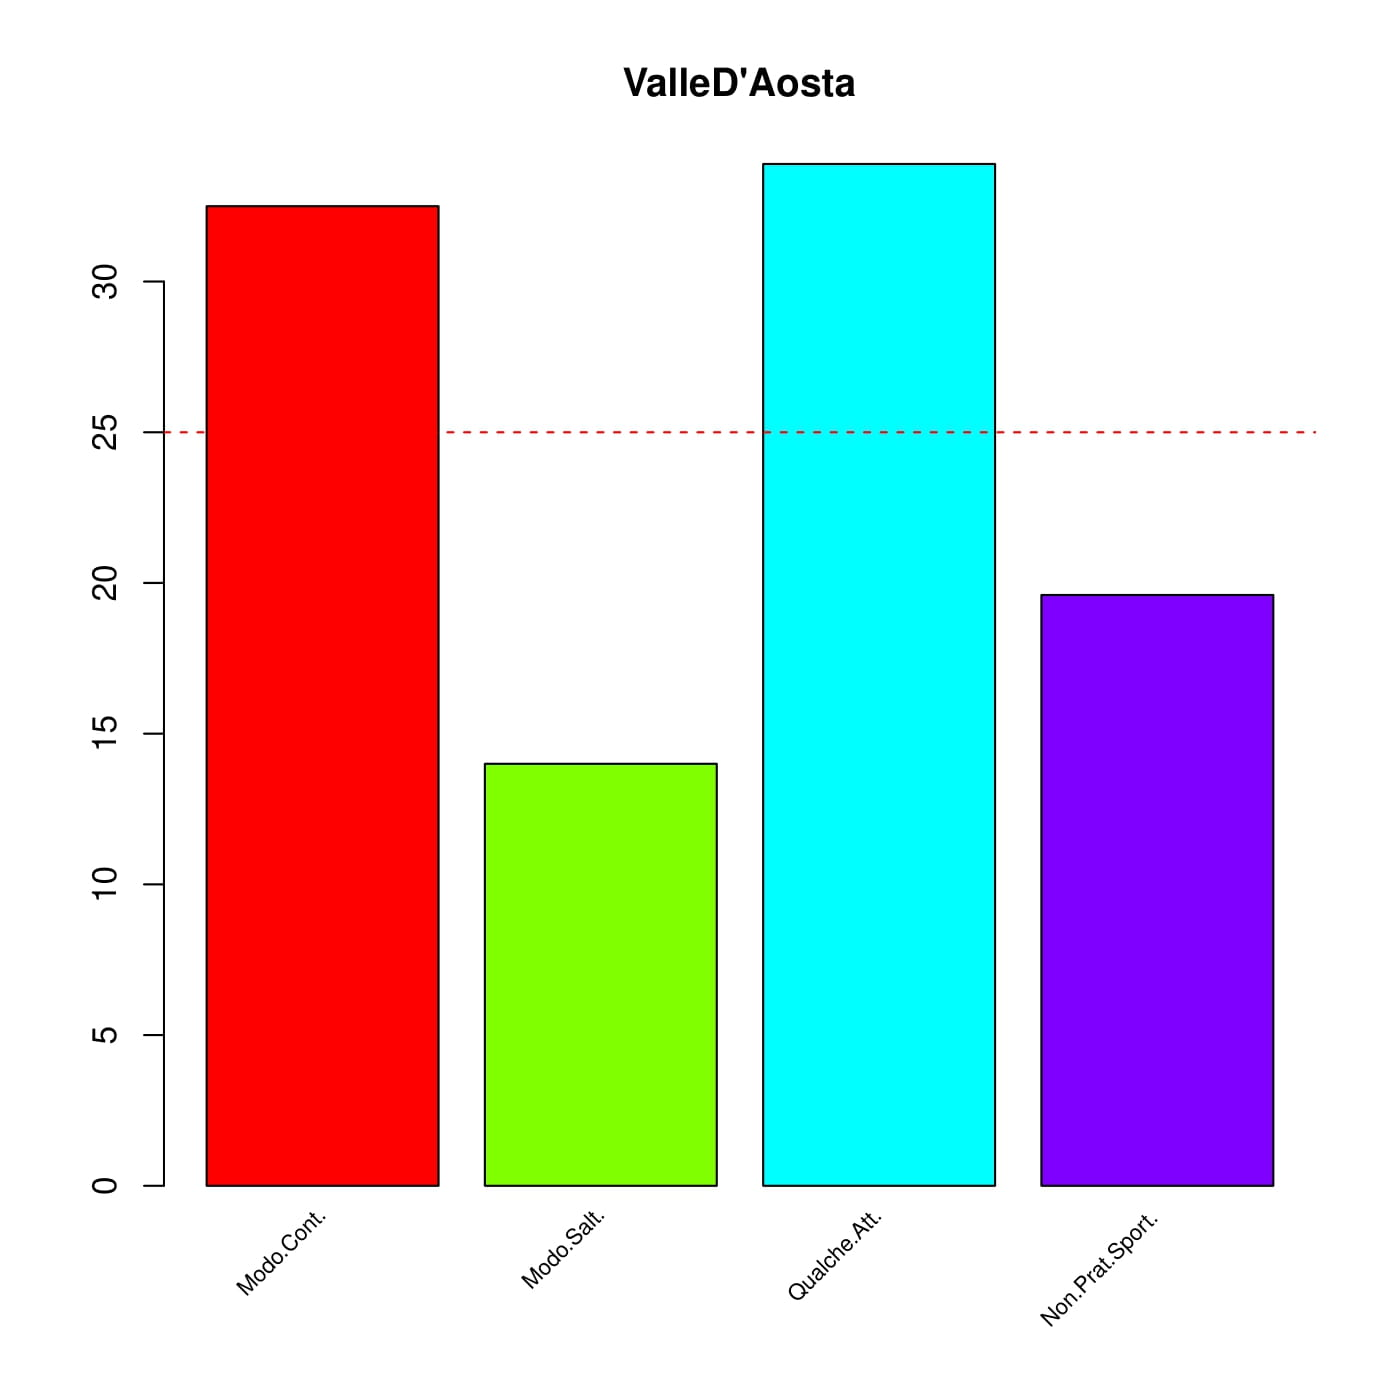
\includegraphics[height=8cm]{ProgettoSAD/capitoli/images/barre_regioni/barre_valledaosta.jpg}}
        \qquad
\end{figure}

\begin{figure}[!htbp]
    \centering
        \subfloat{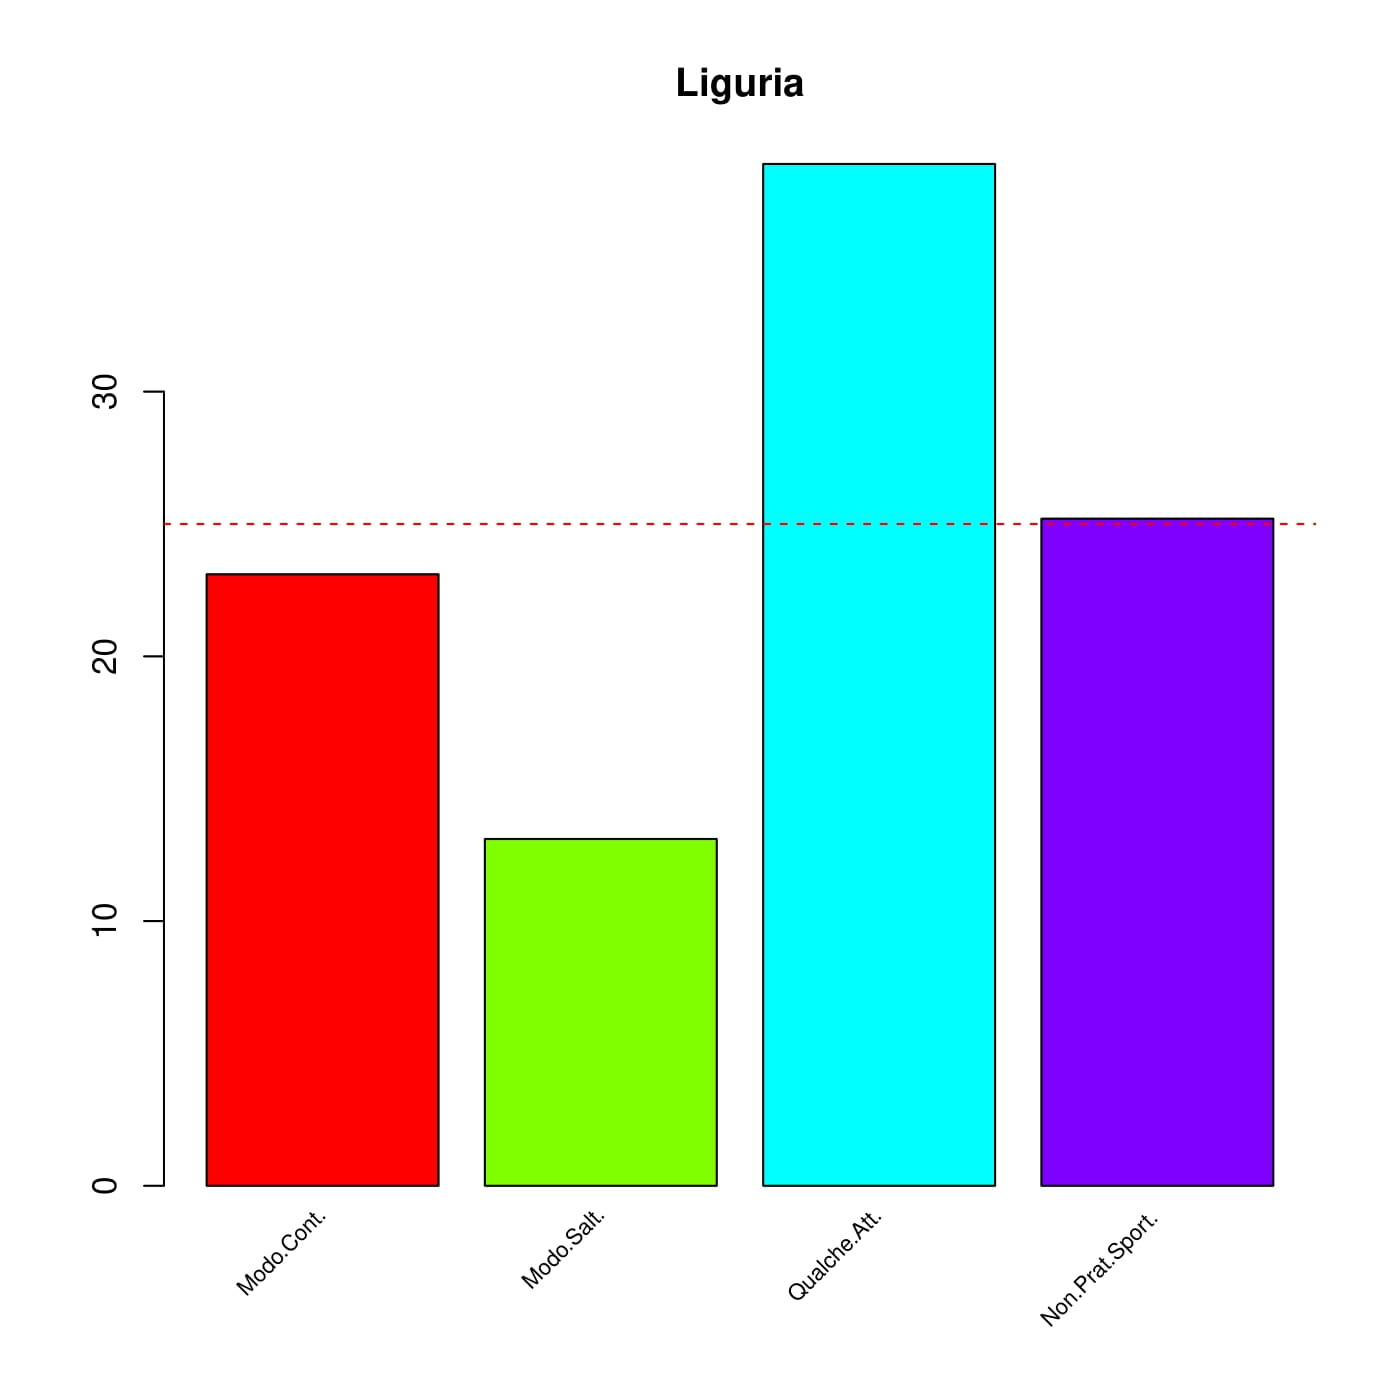
\includegraphics[height=8cm]{ProgettoSAD/capitoli/images/barre_regioni/barre_liguria.jpg}}
        \qquad
        \subfloat{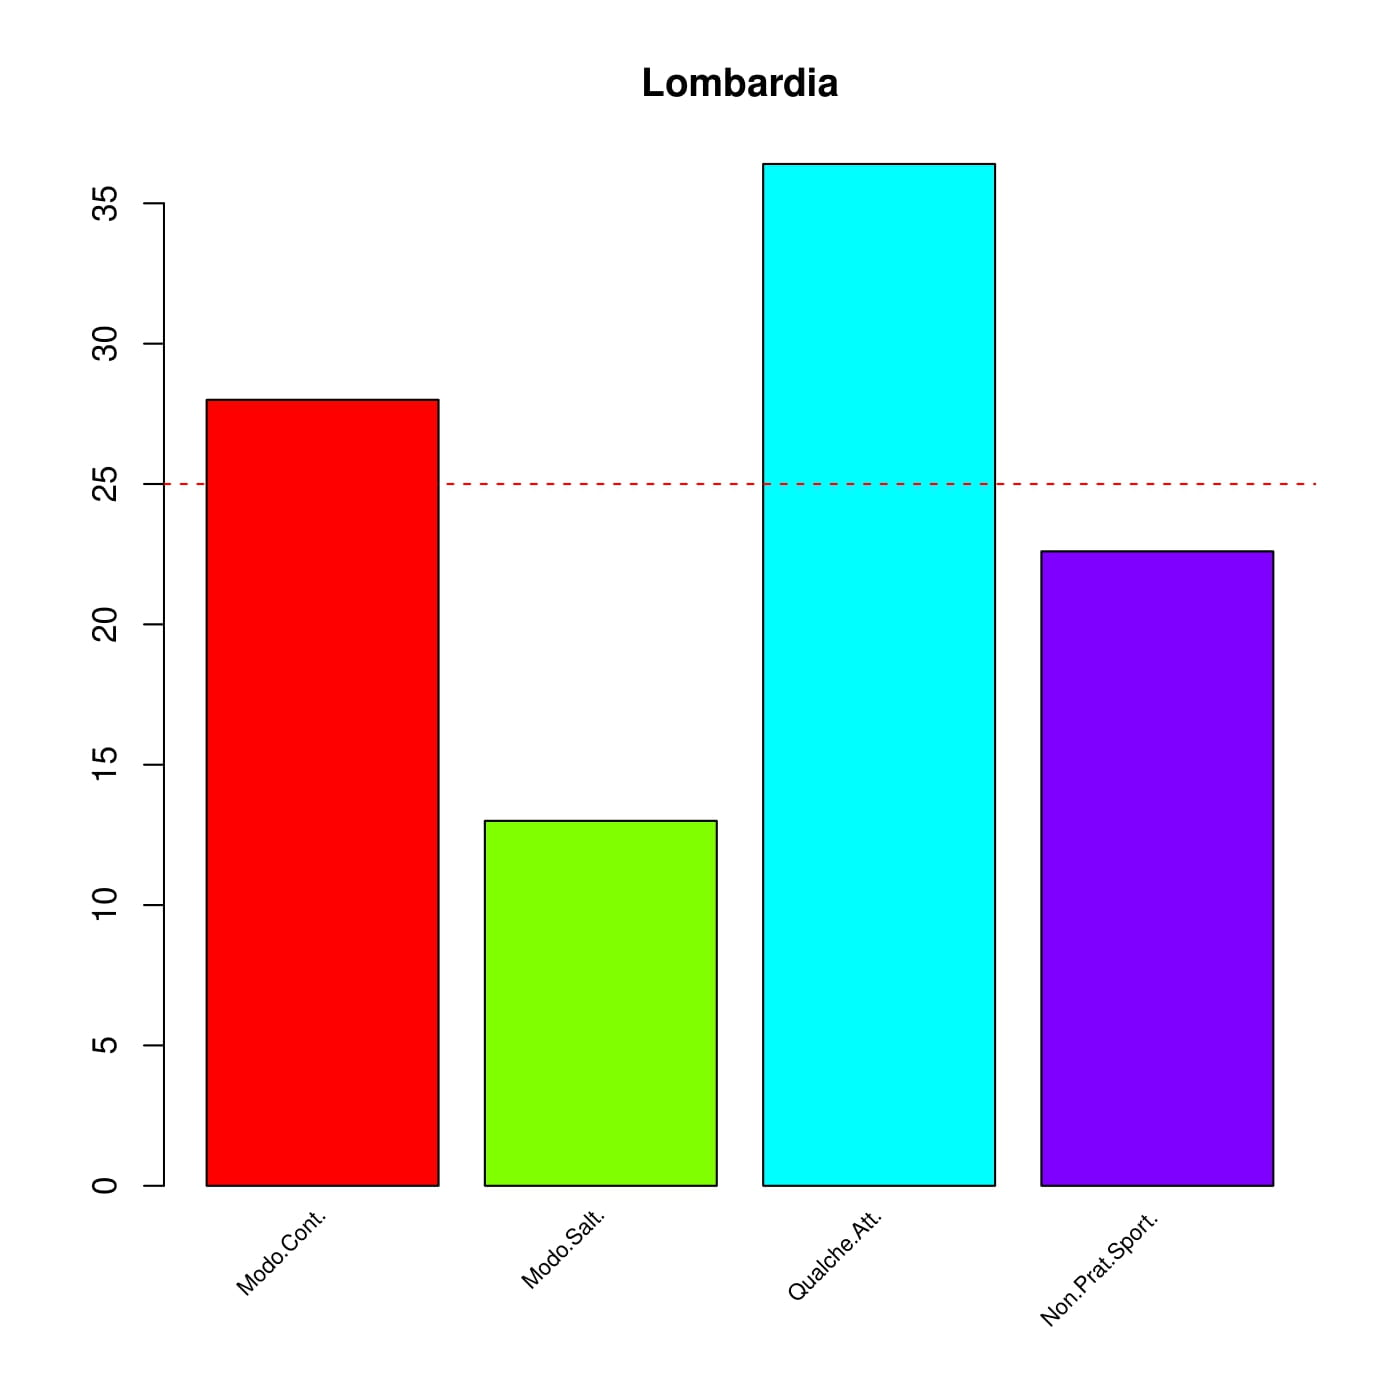
\includegraphics[height=8cm]{ProgettoSAD/capitoli/images/barre_regioni/barre_lombardia.jpg}}
        \qquad
\end{figure}

\begin{figure}[!htbp]
    \centering
        \subfloat{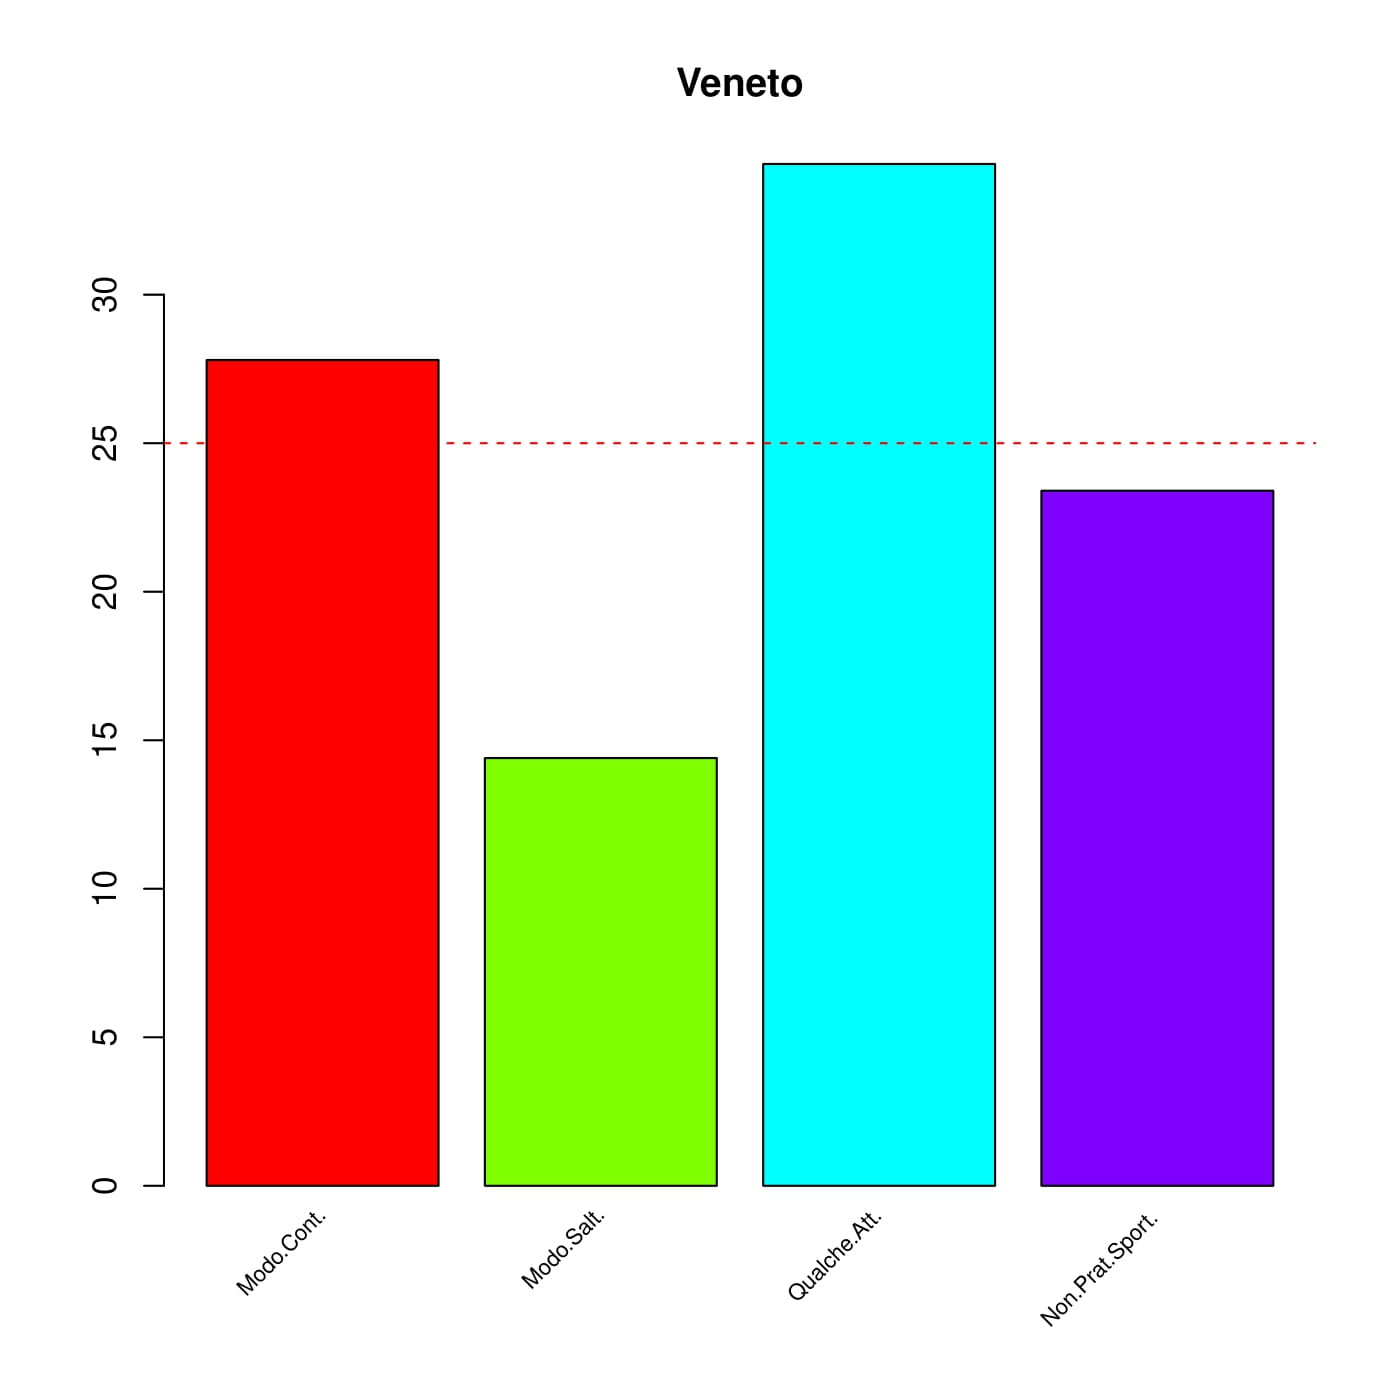
\includegraphics[height=8cm]{ProgettoSAD/capitoli/images/barre_regioni/barre_veneto.jpg}}
        \qquad
        \subfloat{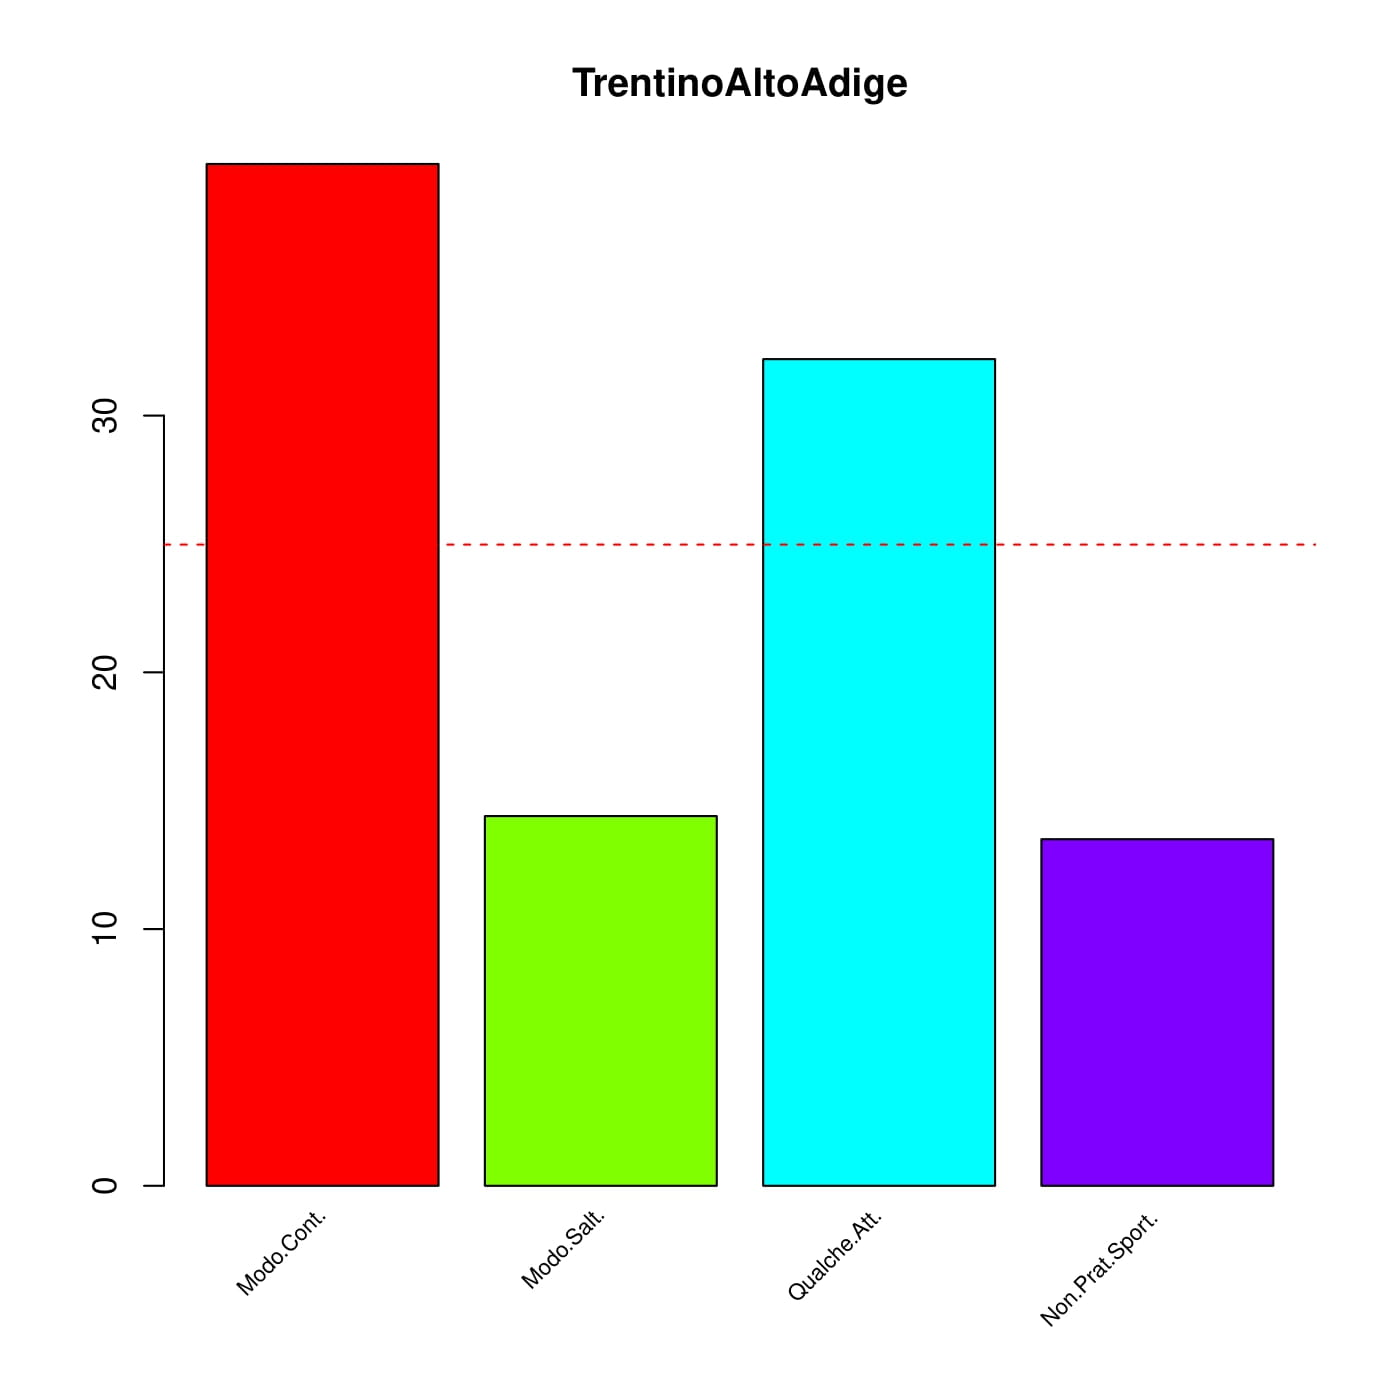
\includegraphics[height=8cm]{ProgettoSAD/capitoli/images/barre_regioni/barre_trentino.jpg}}
        \qquad
\end{figure}

\begin{figure}[!htbp]
    \centering
        \subfloat{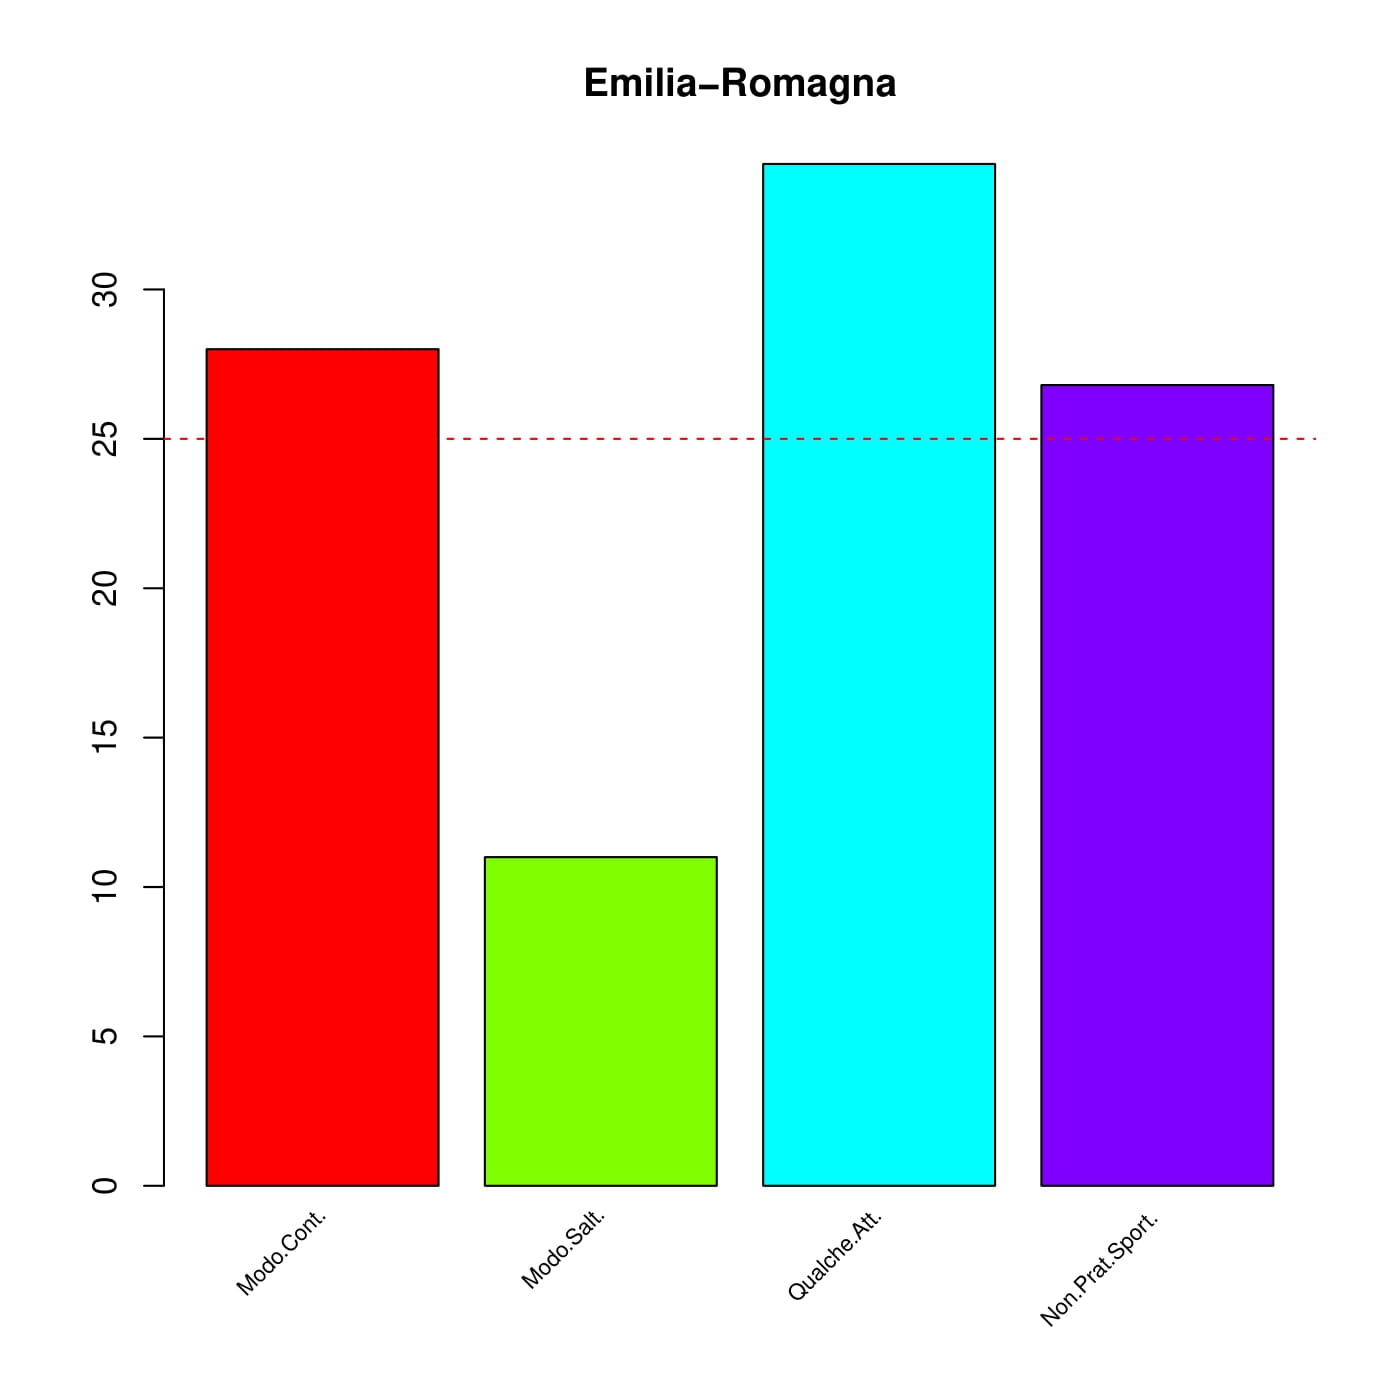
\includegraphics[height=8cm]{ProgettoSAD/capitoli/images/barre_regioni/barre_emilia.jpg}}
        \qquad
        \subfloat{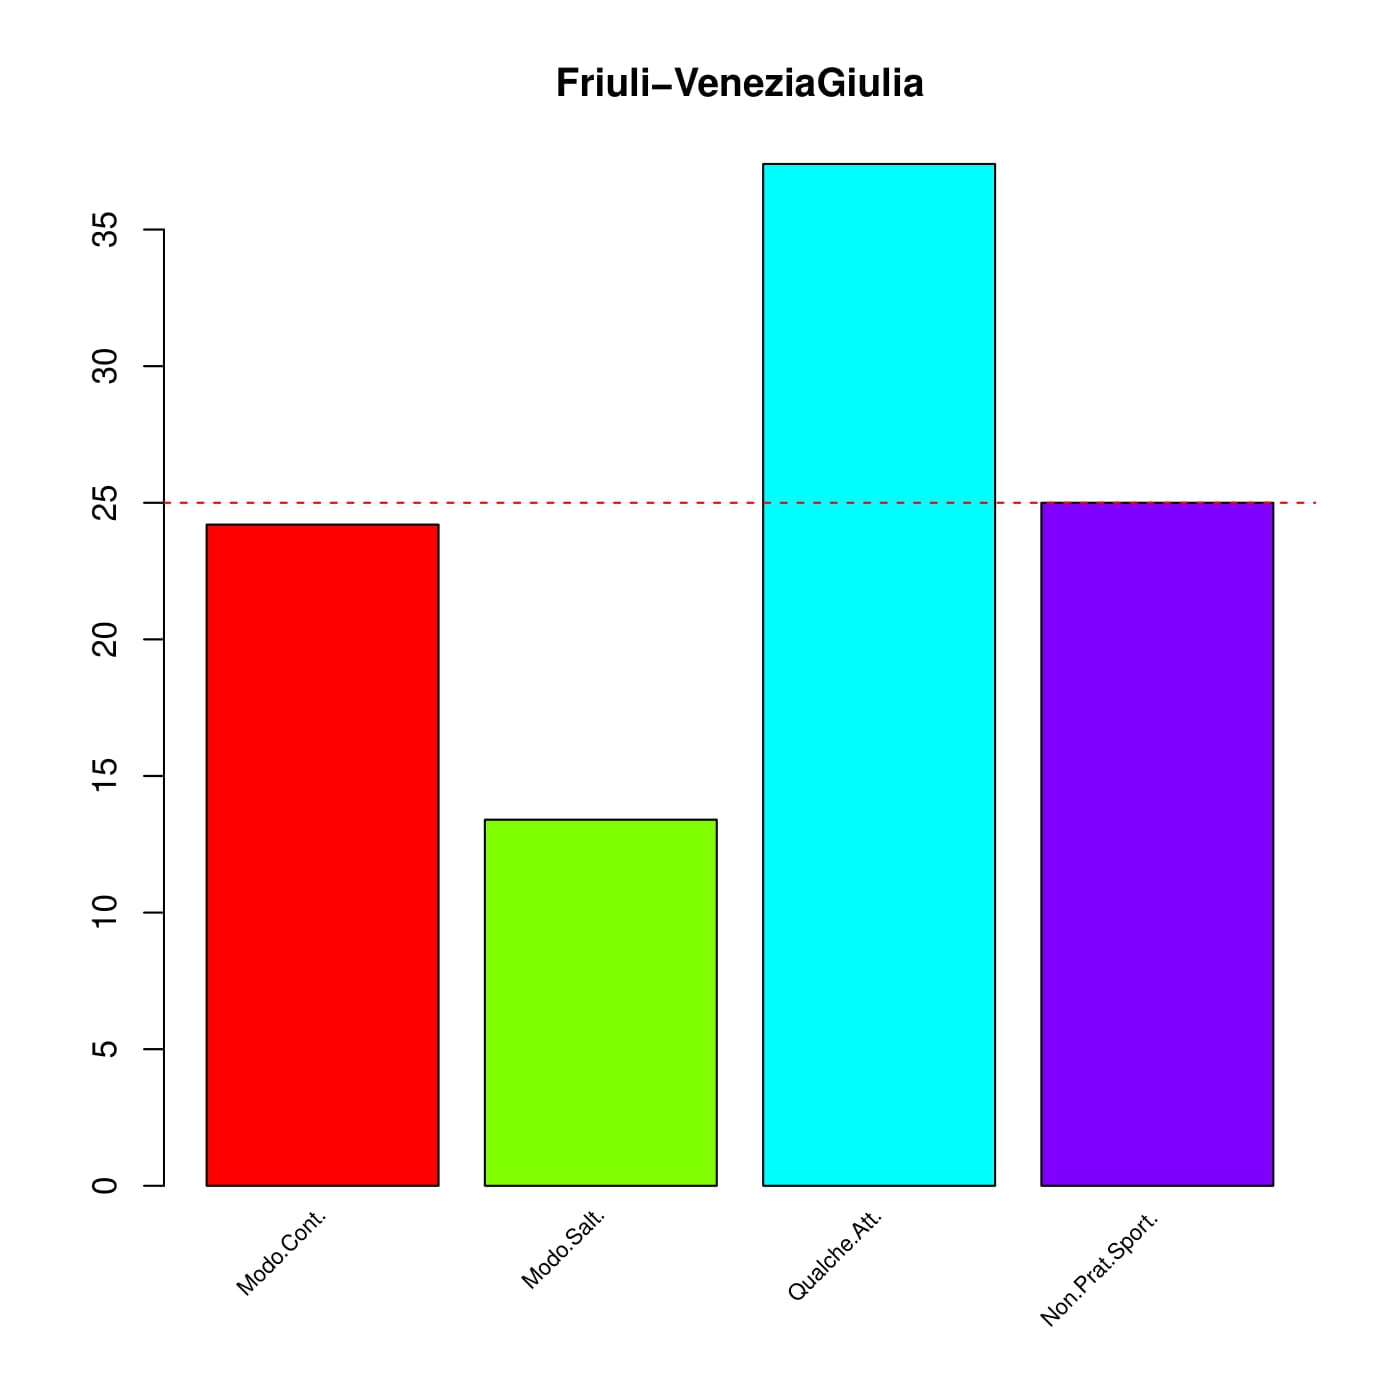
\includegraphics[height=8cm]{ProgettoSAD/capitoli/images/barre_regioni/barre_friuli.jpg}}
        \qquad
\end{figure}

\begin{figure}[!htbp]
    \centering
        \subfloat{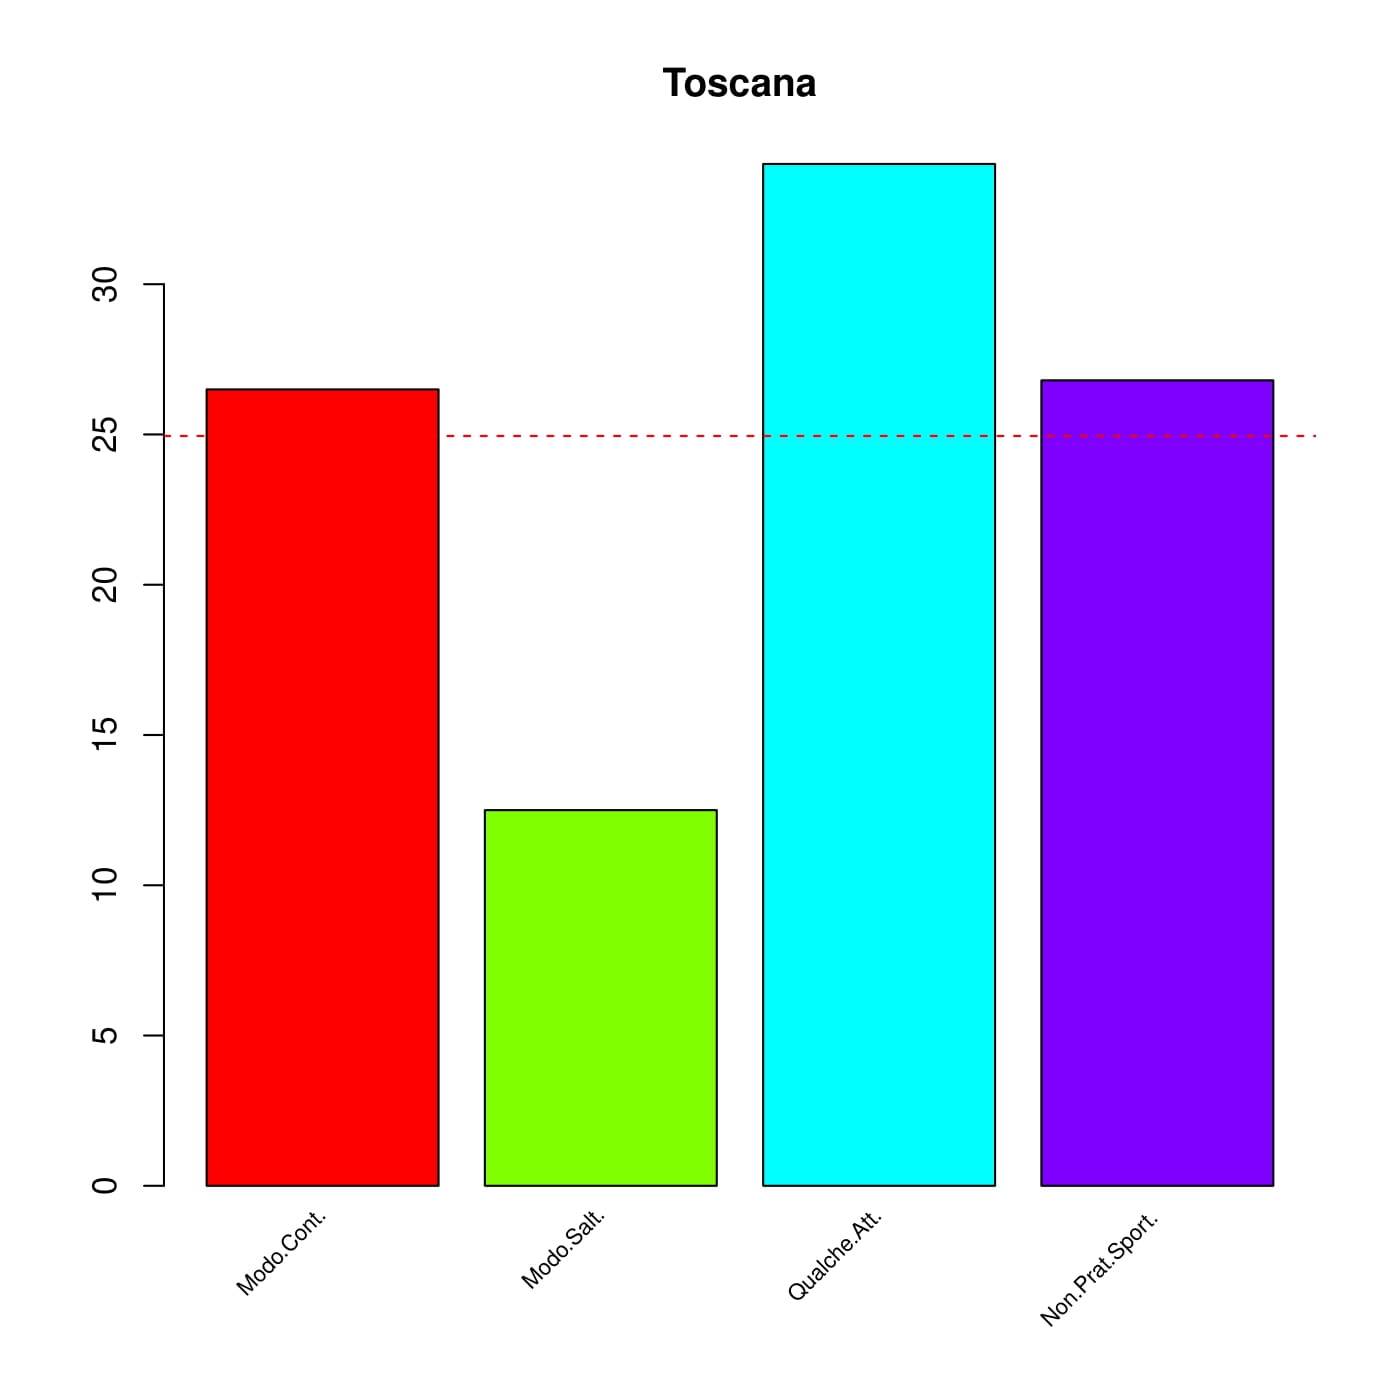
\includegraphics[height=8cm]{ProgettoSAD/capitoli/images/barre_regioni/barre_toscana.jpg}}
        \qquad
        \subfloat{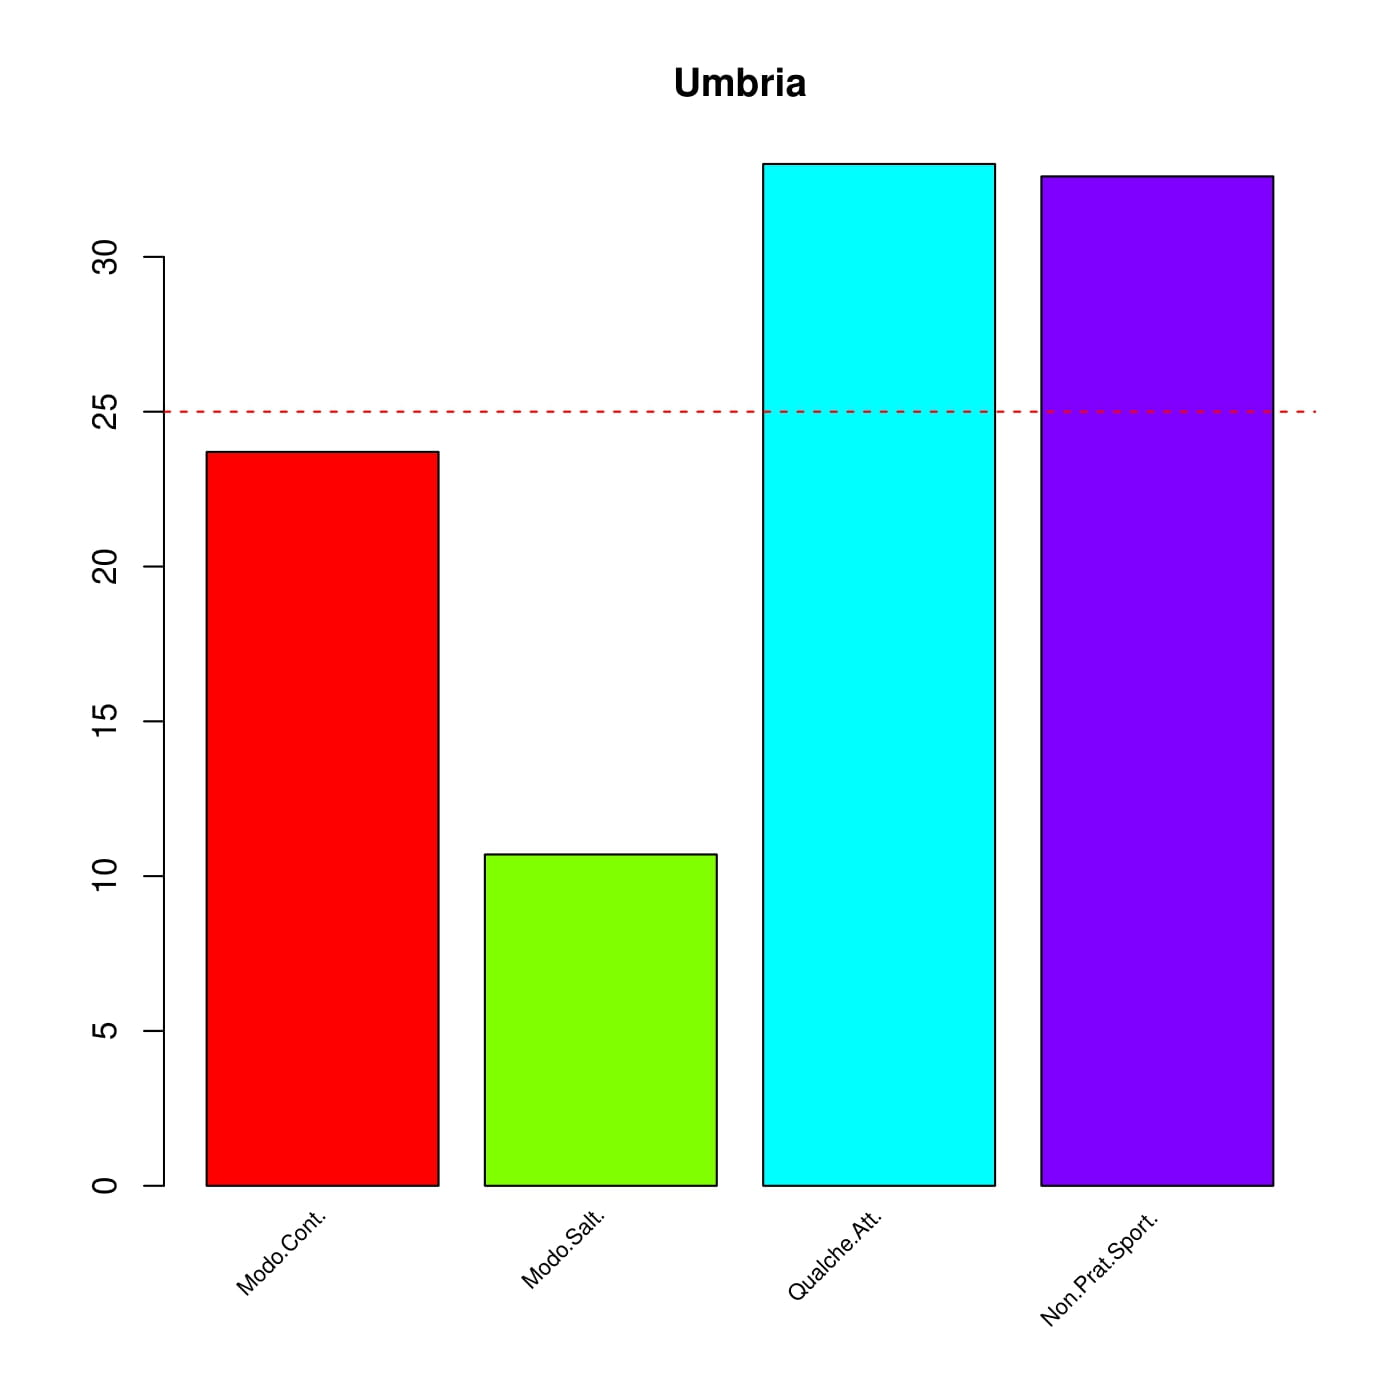
\includegraphics[height=8cm]{ProgettoSAD/capitoli/images/barre_regioni/barre_umbria.jpg}}
        \qquad
\end{figure}

\begin{figure}[!htbp]
    \centering
        \subfloat{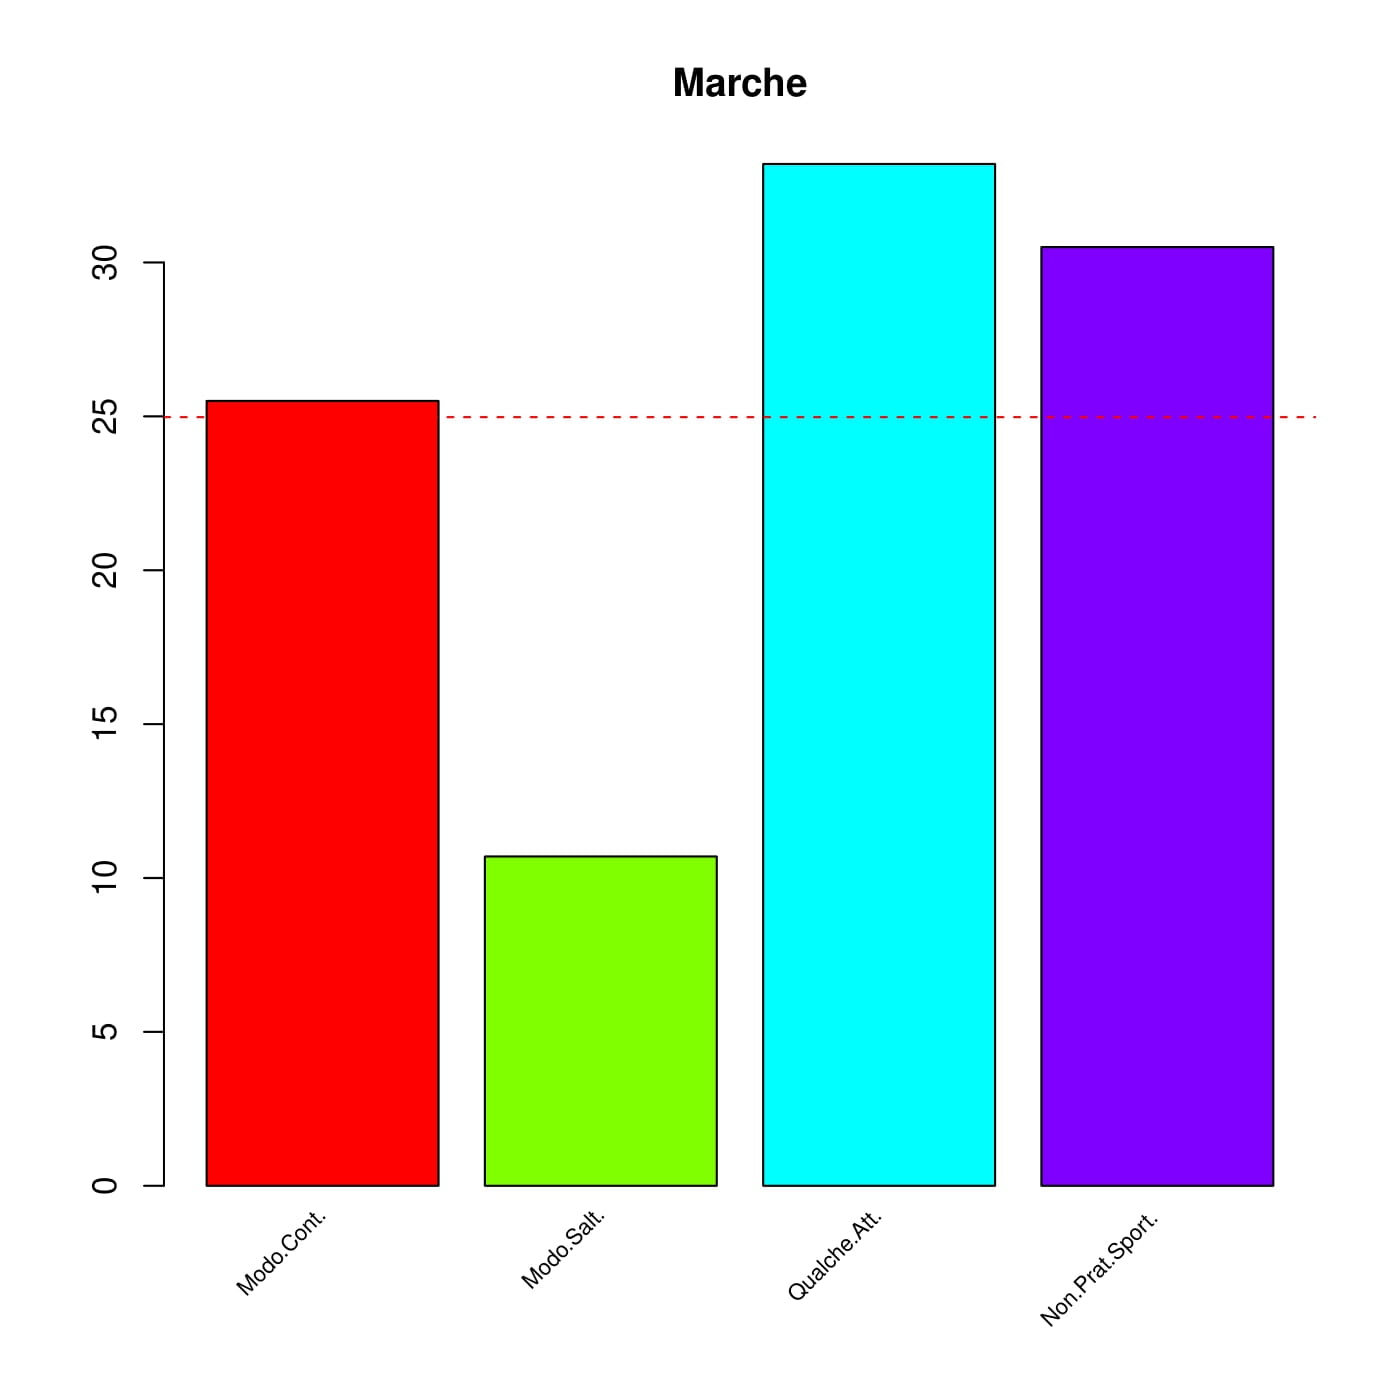
\includegraphics[height=8cm]{ProgettoSAD/capitoli/images/barre_regioni/barre_marche.jpg}}
        \qquad
        \subfloat{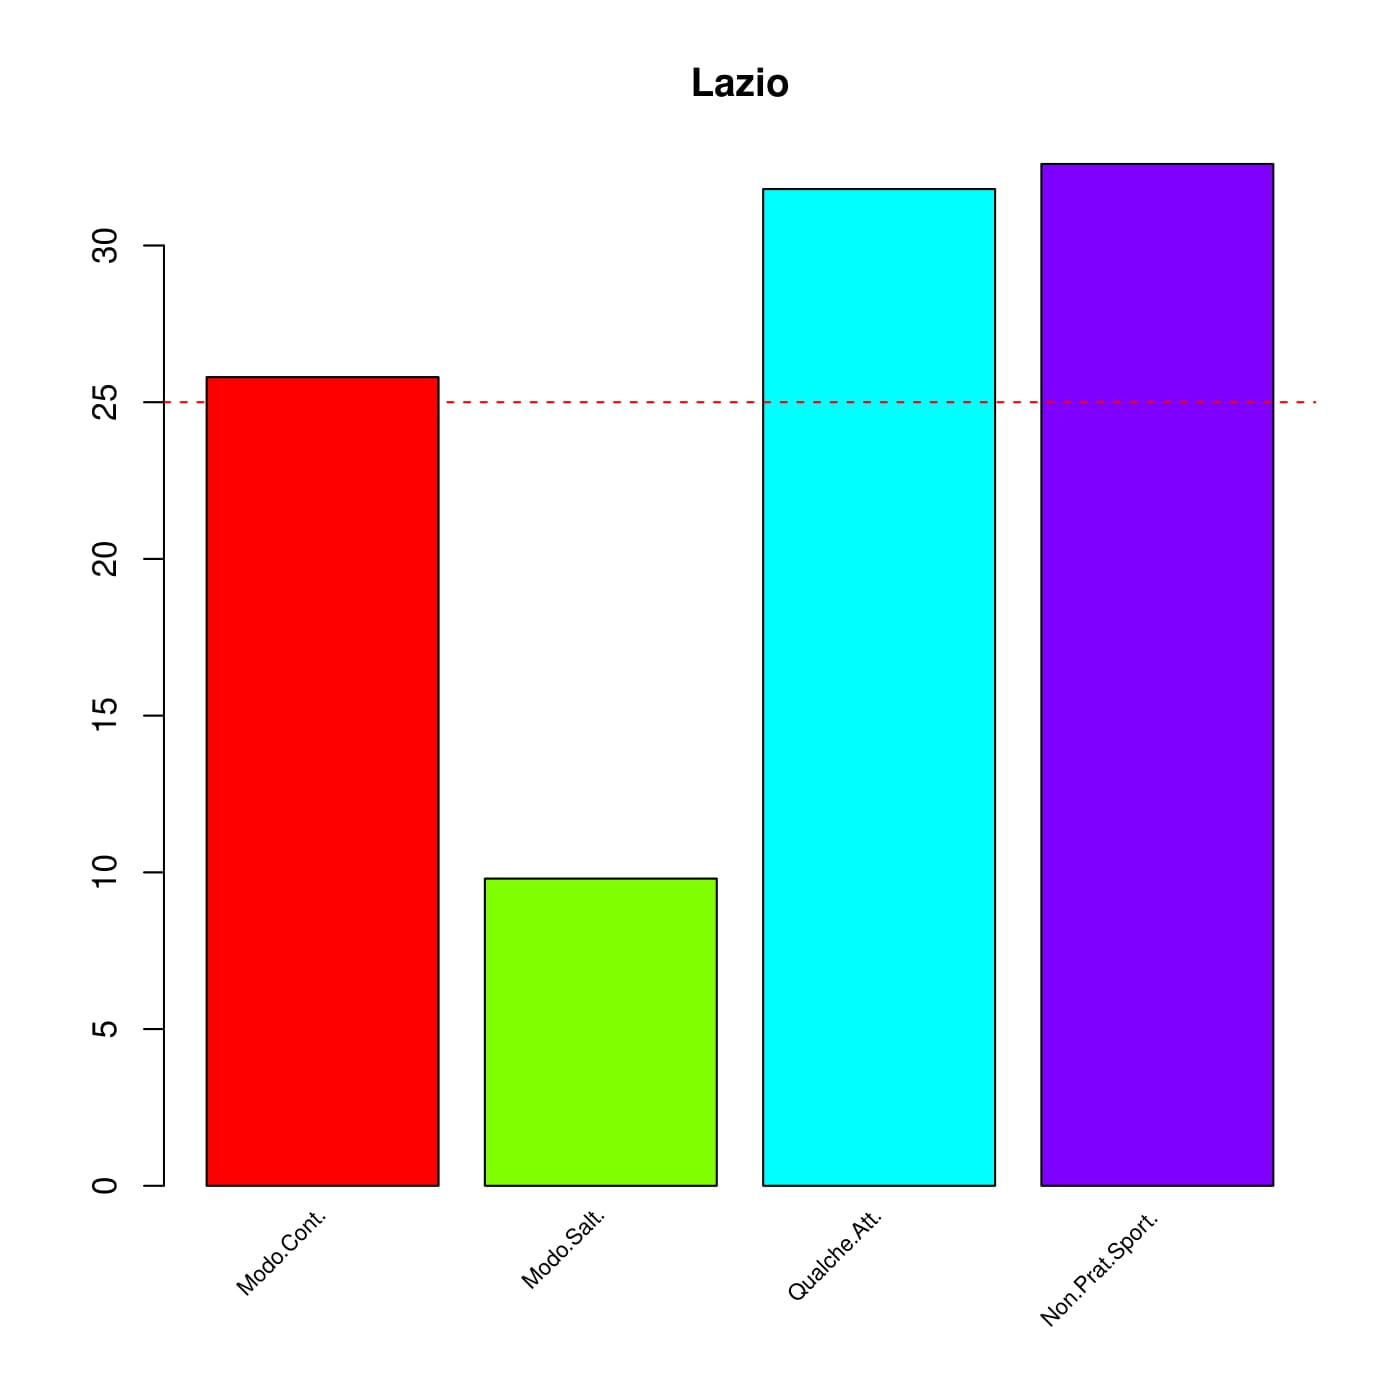
\includegraphics[height=8cm]{ProgettoSAD/capitoli/images/barre_regioni/barre_lazio.jpg}}
        \qquad
\end{figure}

\begin{figure}[!htbp]
    \centering
        \subfloat{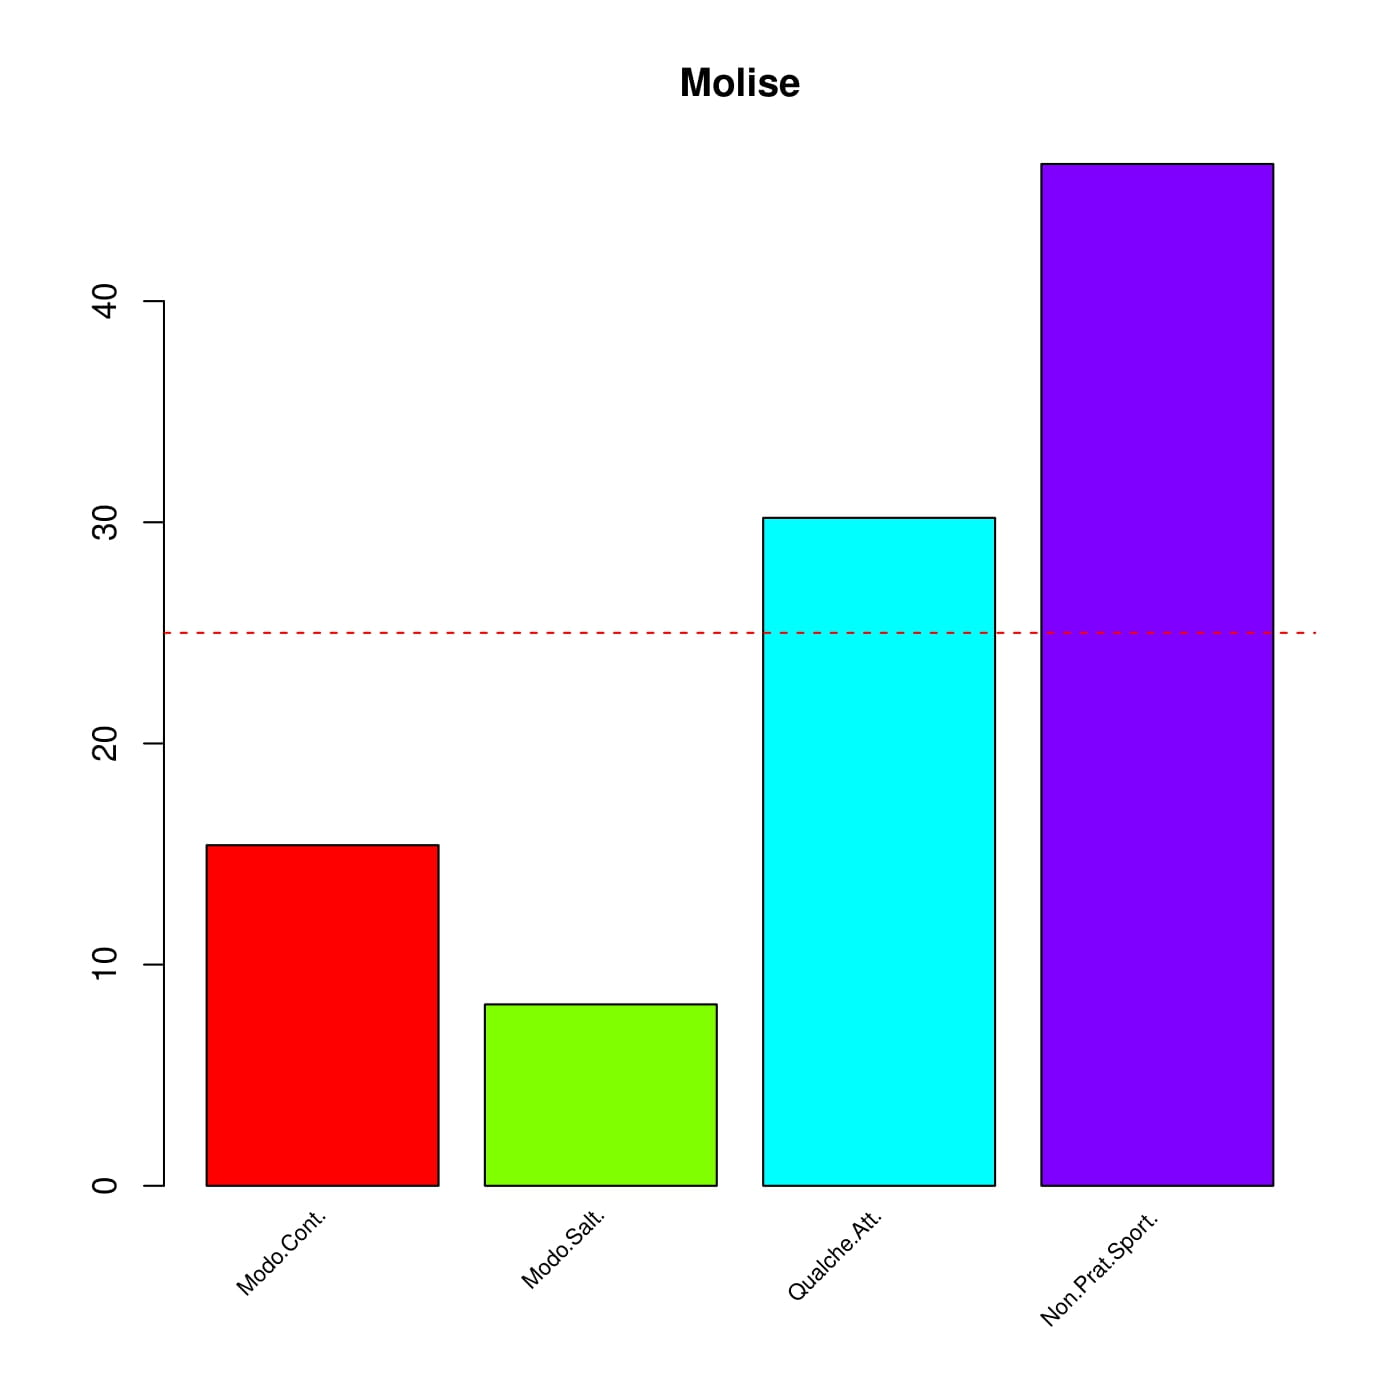
\includegraphics[height=8cm]{ProgettoSAD/capitoli/images/barre_regioni/barre_molise.jpg}}
        \qquad
        \subfloat{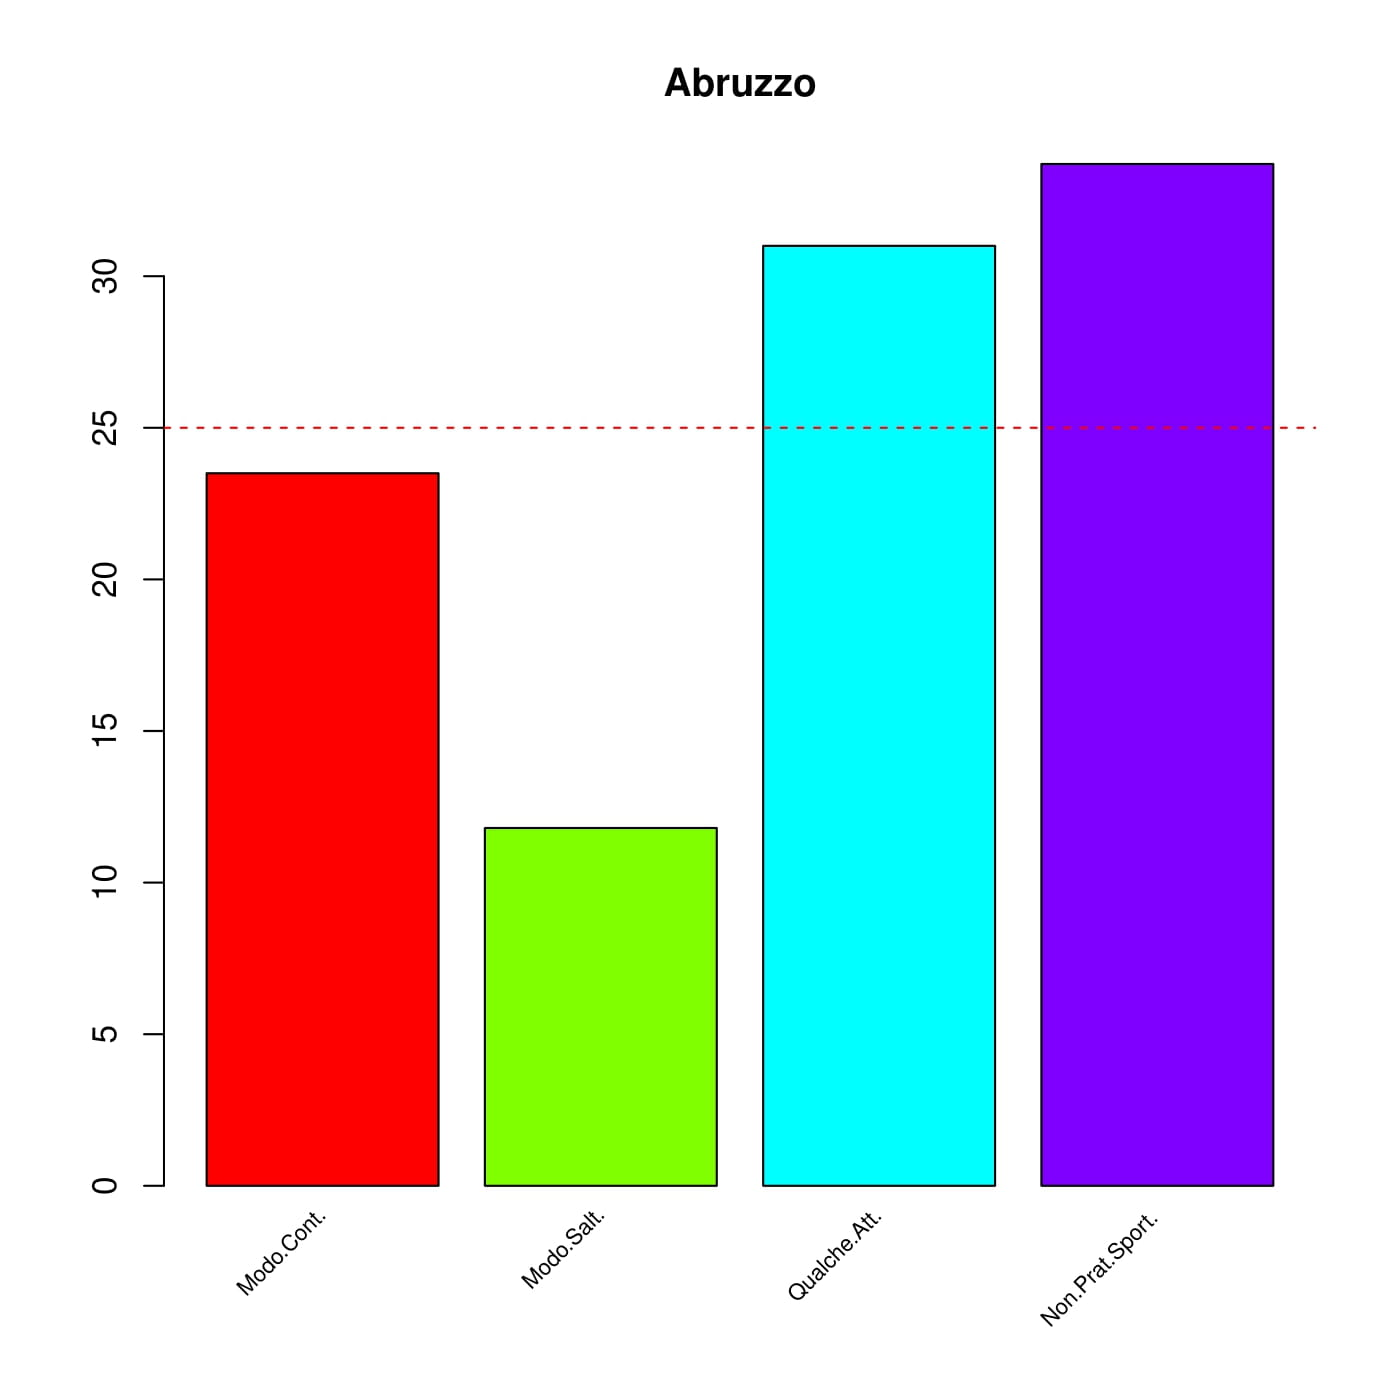
\includegraphics[height=8cm]{ProgettoSAD/capitoli/images/barre_regioni/barre_abruzzo.jpg}}
        \qquad
\end{figure}

\begin{figure}[!htbp]
    \centering
        \subfloat{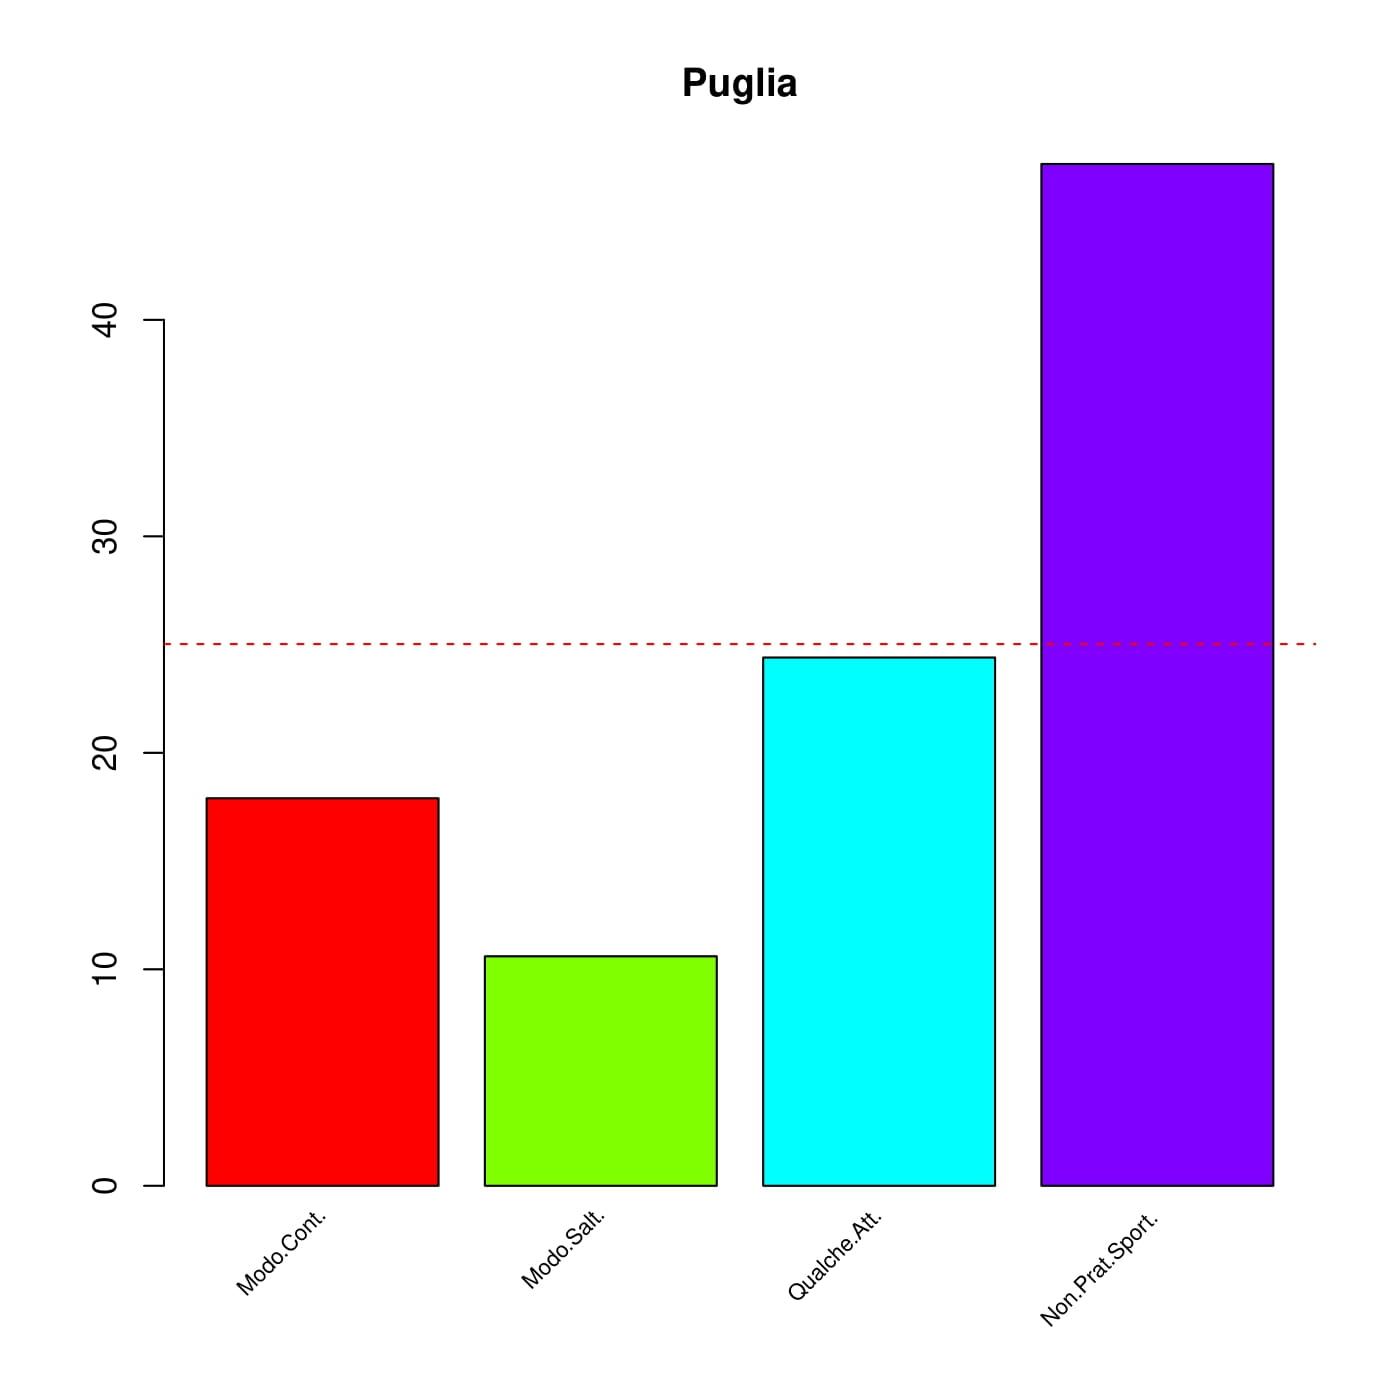
\includegraphics[height=8cm]{ProgettoSAD/capitoli/images/barre_regioni/barre_puglia.jpg}}
        \qquad
        \subfloat{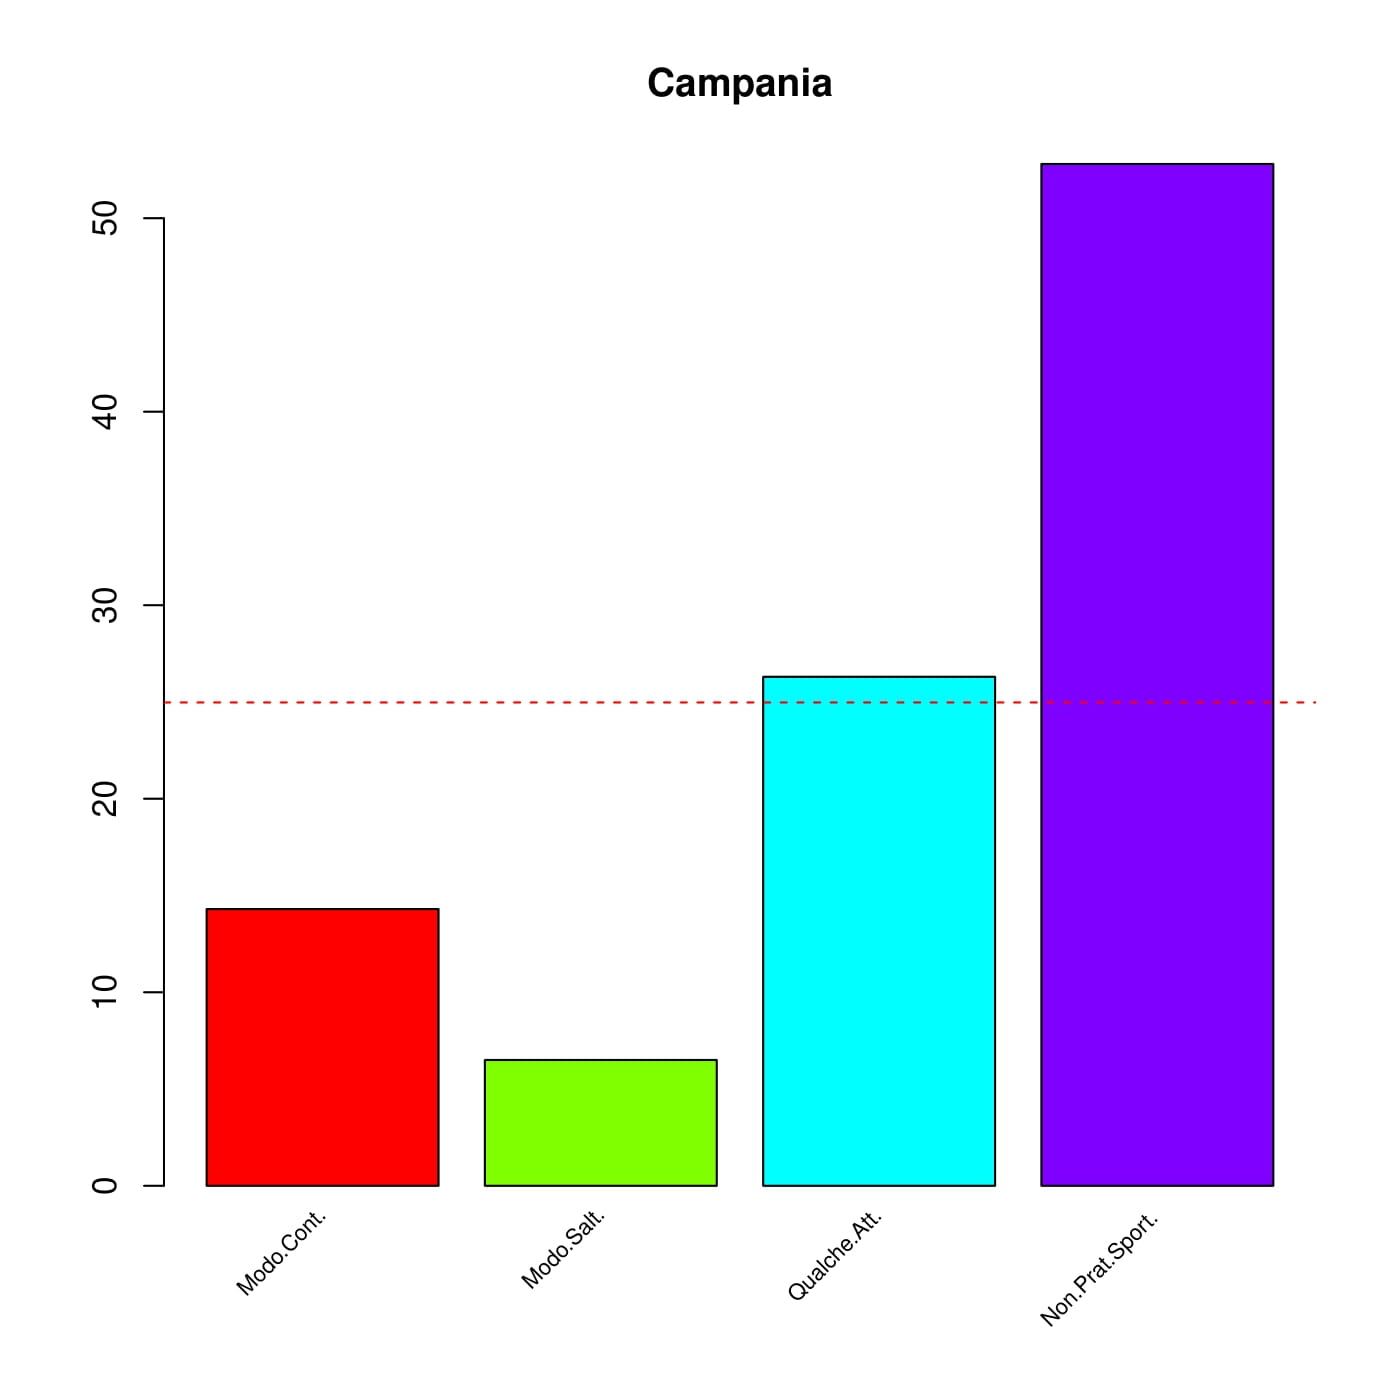
\includegraphics[height=8cm]{ProgettoSAD/capitoli/images/barre_regioni/barre_campania.jpg}}
        \qquad
\end{figure}

\begin{figure}[!htbp]
    \centering
        \subfloat{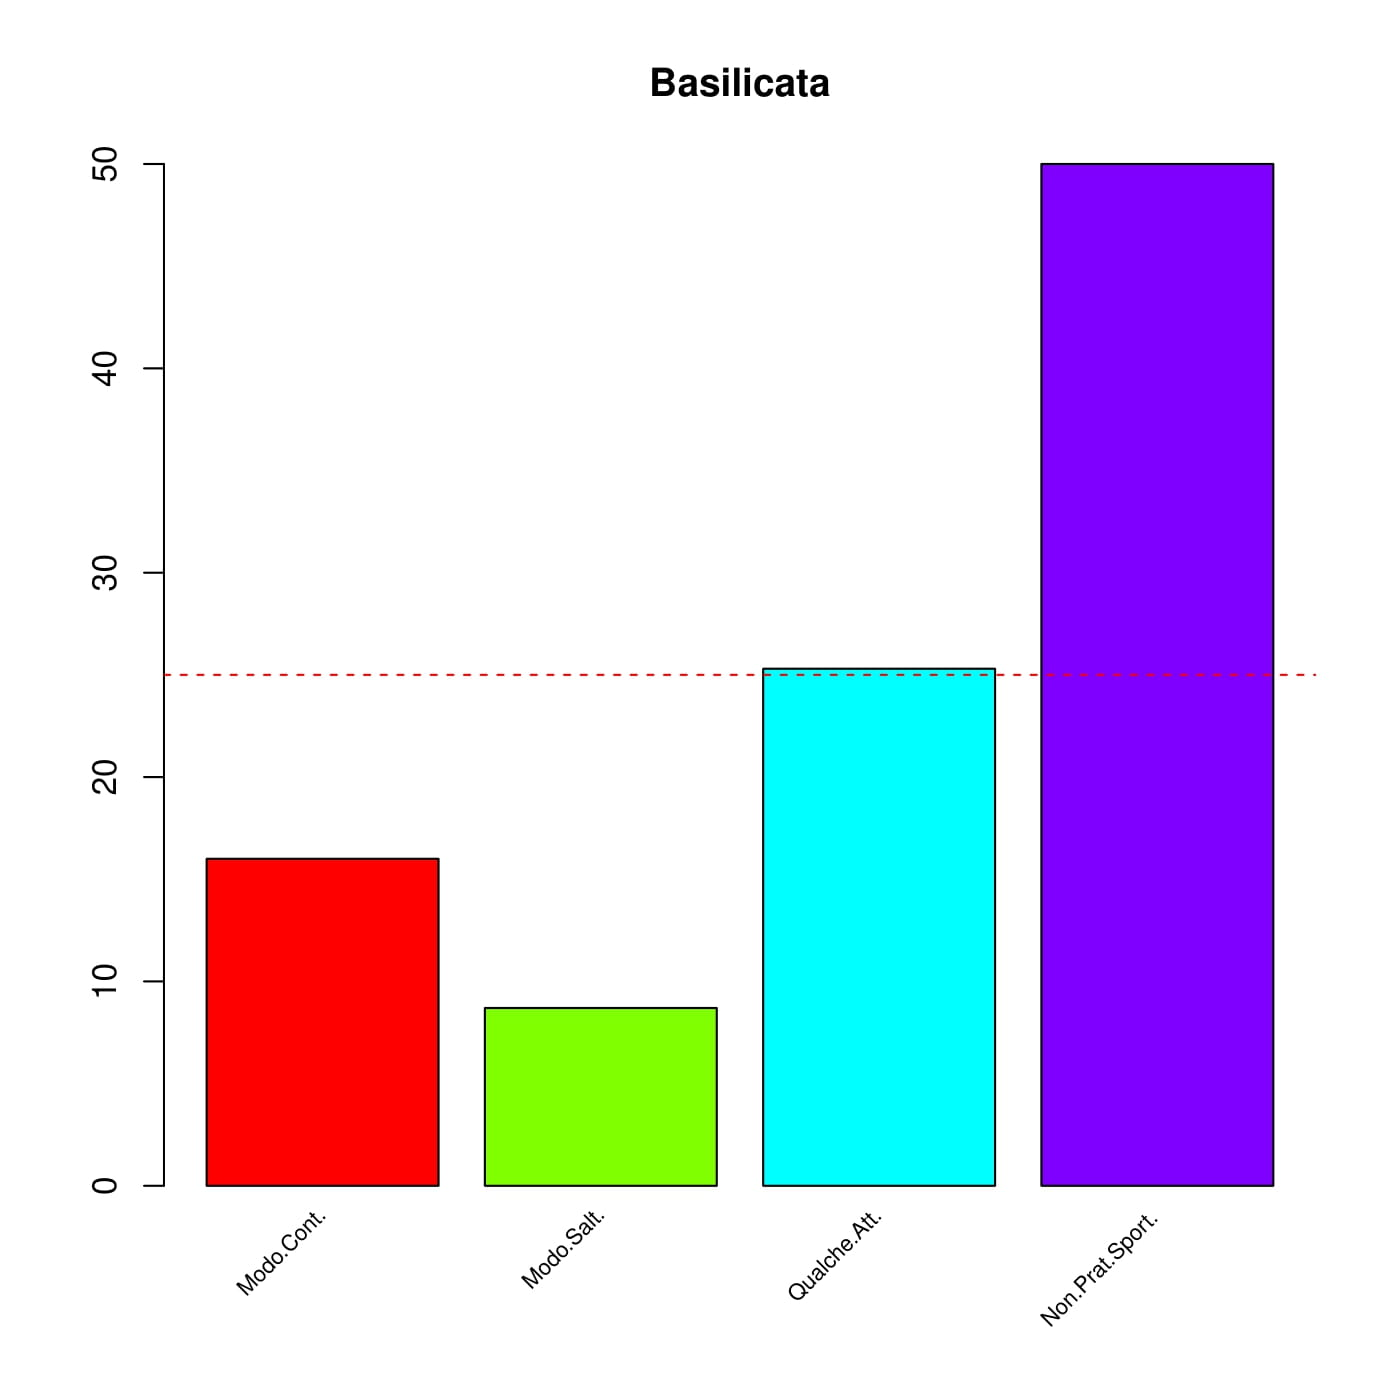
\includegraphics[height=8cm]{ProgettoSAD/capitoli/images/barre_regioni/barre_basilicata.jpg}}
        \qquad
        \subfloat{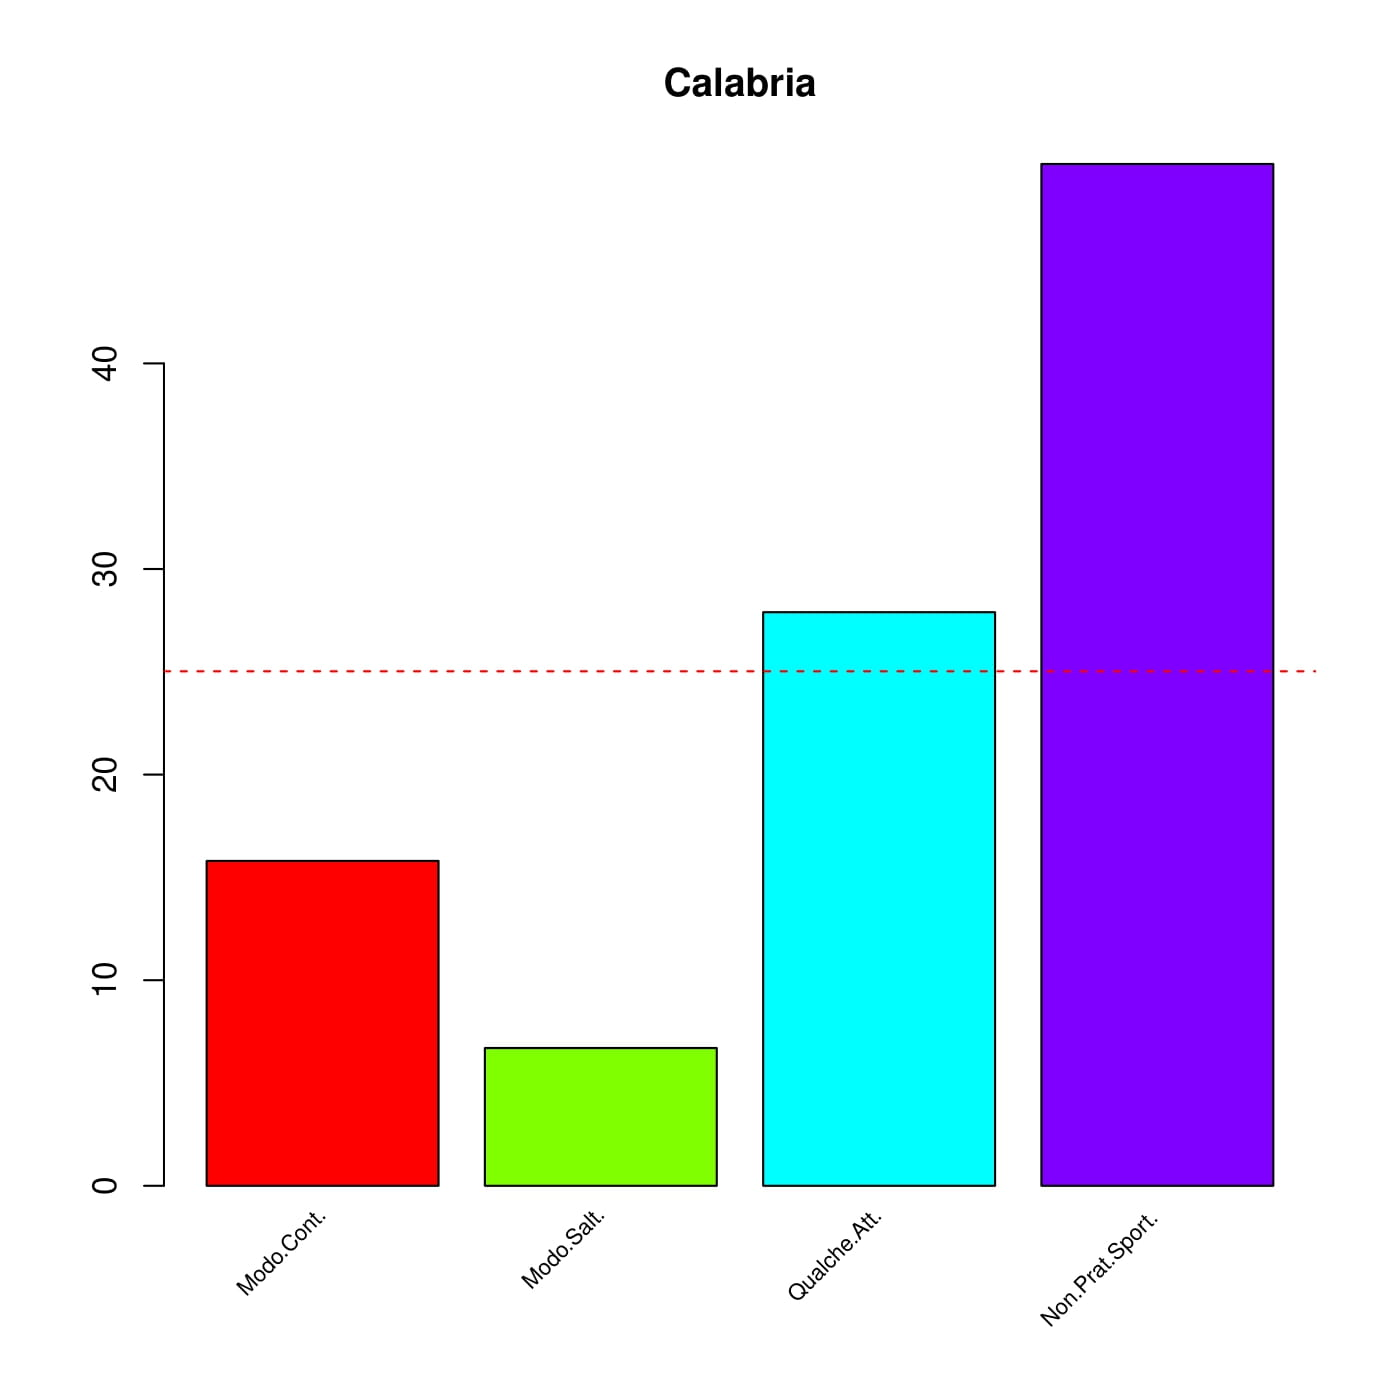
\includegraphics[height=8cm]{ProgettoSAD/capitoli/images/barre_regioni/barre_calabria.jpg}}
        \qquad
\end{figure}

\begin{figure}[!htbp]
    \centering
        \subfloat{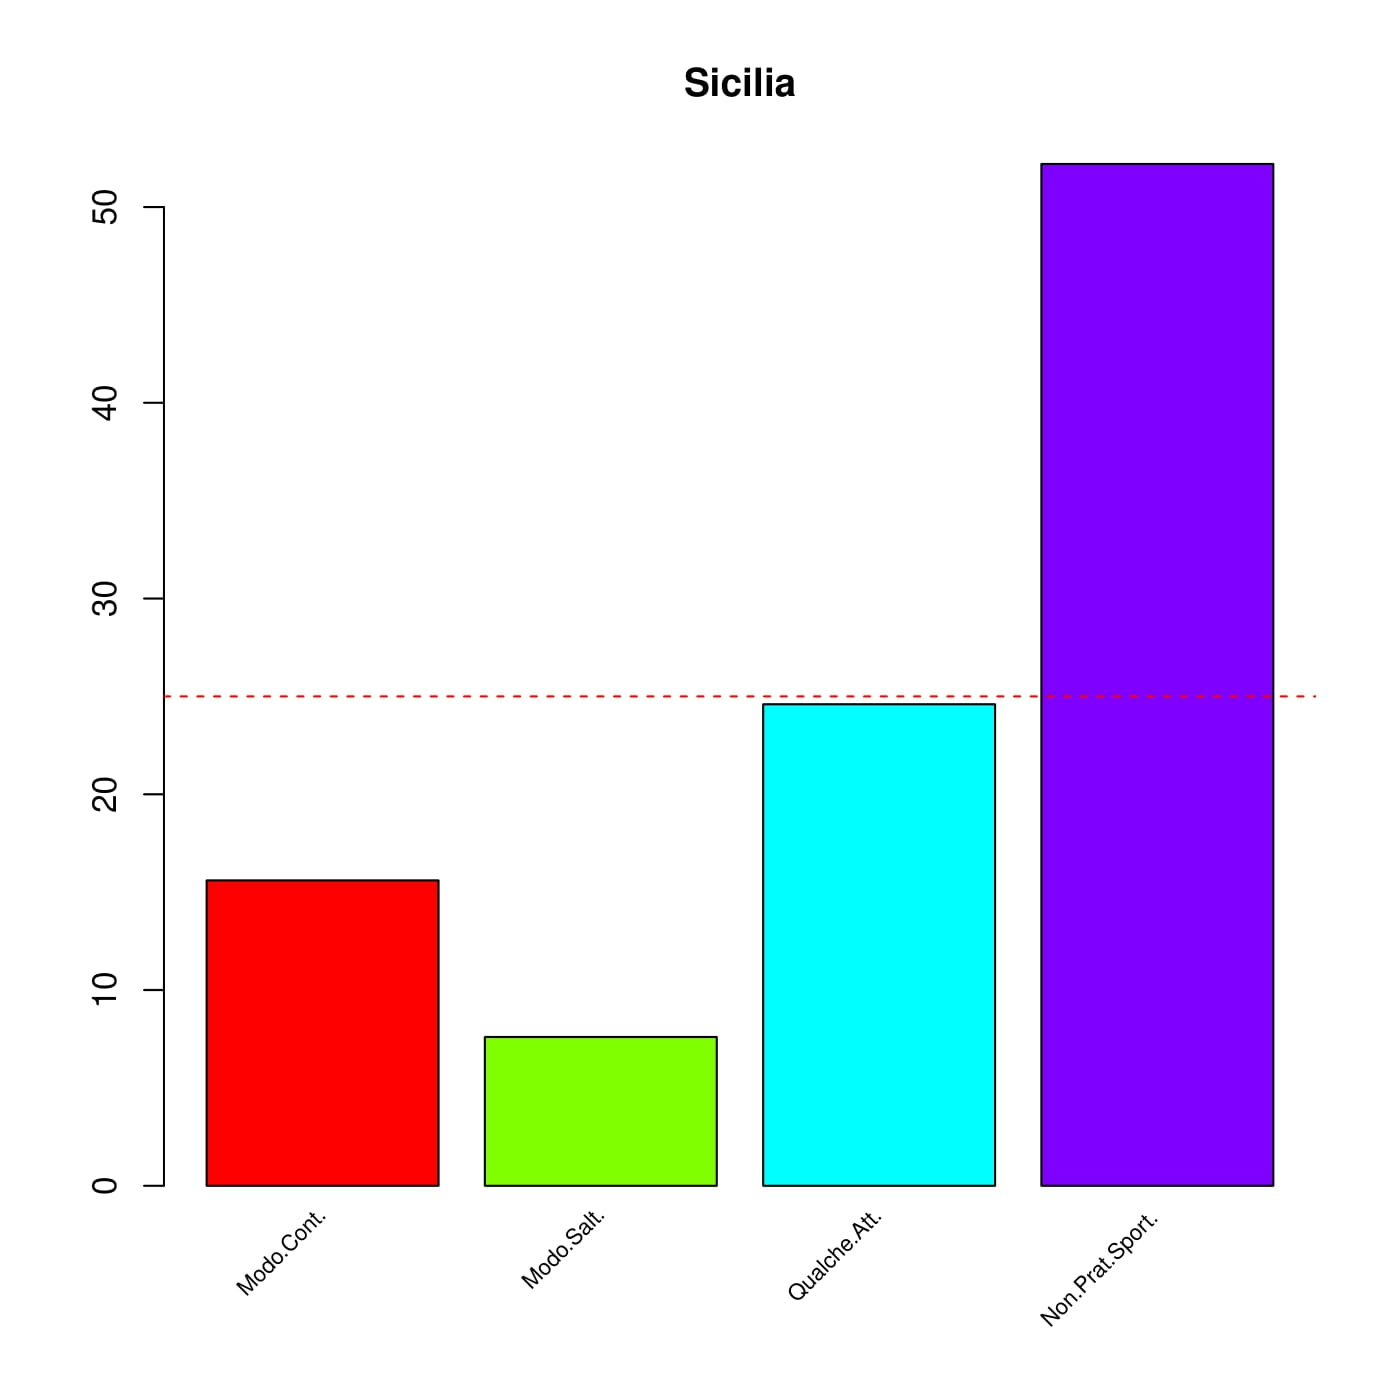
\includegraphics[height=8cm]{ProgettoSAD/capitoli/images/barre_regioni/barre_sicilia.jpg}}
        \qquad
        \subfloat{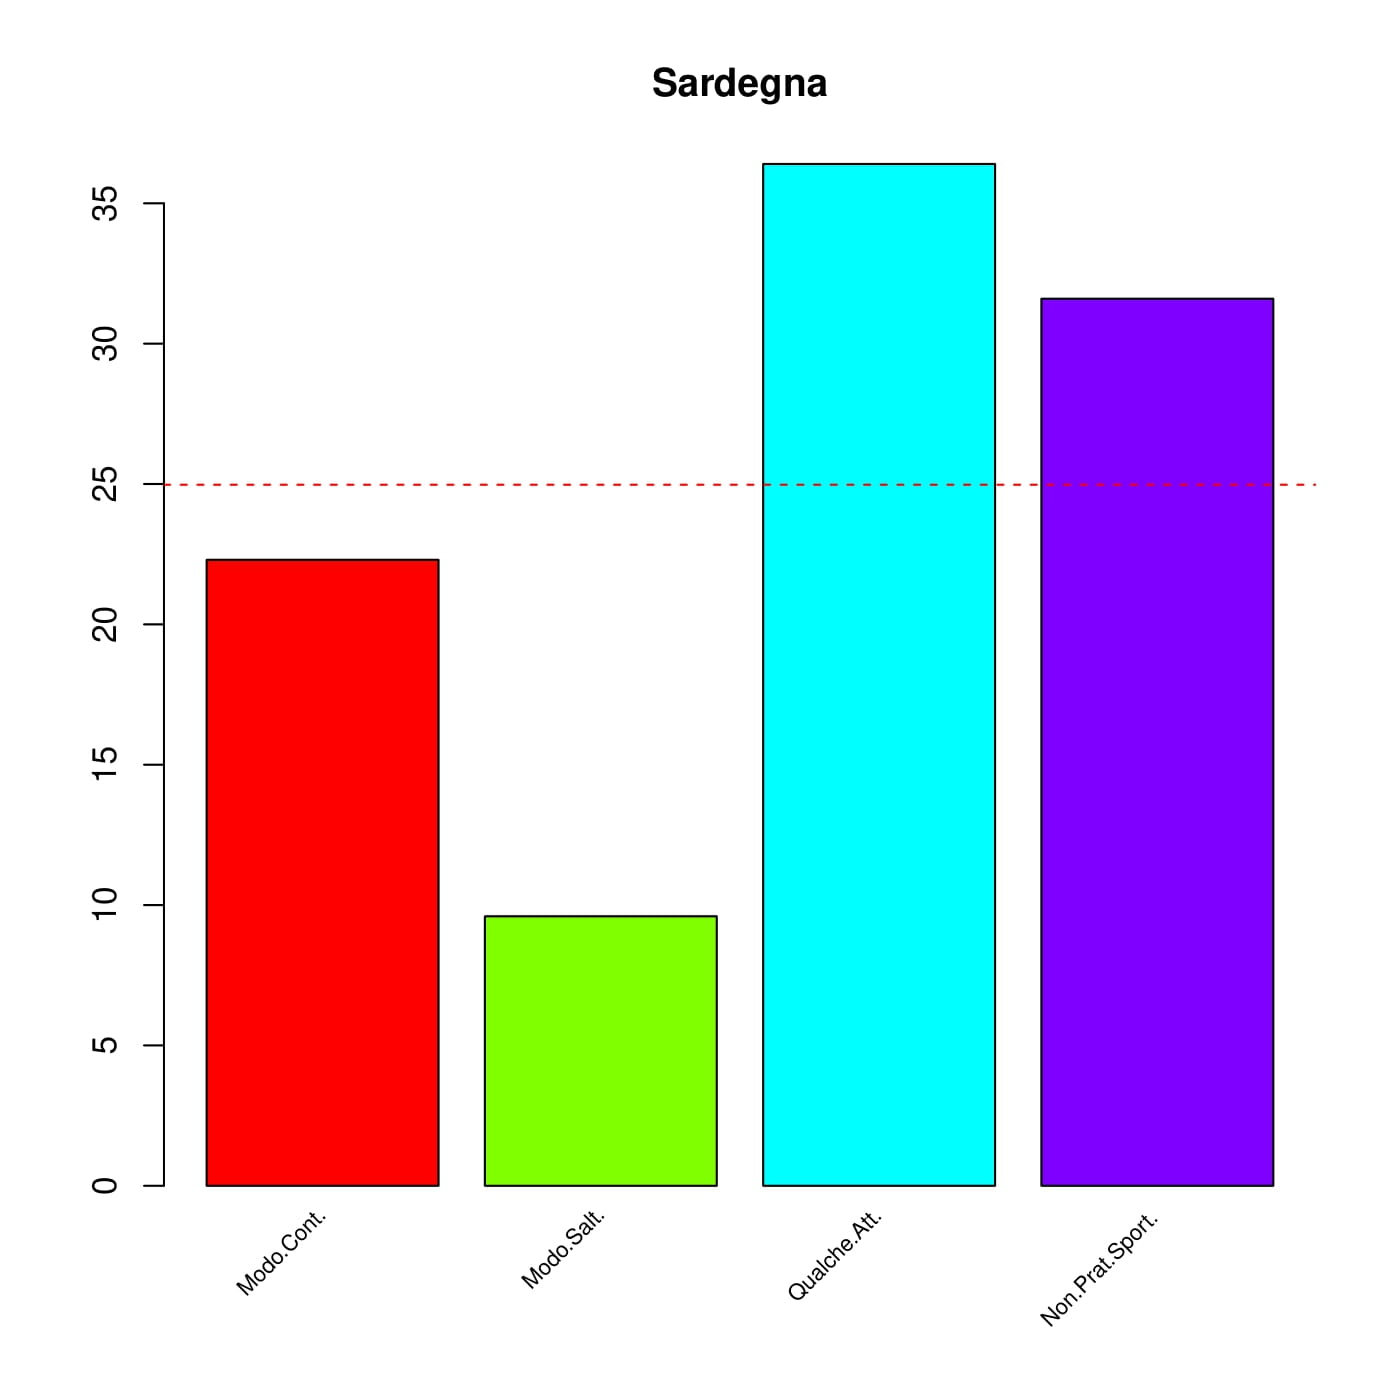
\includegraphics[height=8cm]{ProgettoSAD/capitoli/images/barre_regioni/barre_sardegna.jpg}}
        \qquad
\end{figure}

Dai grafici ottenuti, si può notare che nel Nord e nel centro Italia i più frequenti sono quelli a svolgere attività sportiva costante o qualche attività, mentre nel Sud e nelle Isole a prevalere sono quelli che svolgono qualche attività sportiva o non ne svolgono affatto.



\section{Grafici a torta: Regioni}\label{cap2.3}

In questa sezione verrà mostrato un grafico a torta per ogni regione del dataset, al fine di poter analizzare la densità di pratica sportiva in relazione alla totalità.

\noindent \textbf{Costruzione Grafico a torta}

È possibile impiegare nuovamente la funzione \textit{estraiRiga()} per creare i grafici a torta per le regioni.

\vspace{5mm}
\begin{lstlisting}
 index <- 1
  for (element in regioni) {
    pie1 <- pie(estraiRiga(df, index),
                labels = names(df),
                main = element,
                col = rainbow(5))
    index <- index + 1
  }
\end{lstlisting}
\vspace{5mm}

\begin{figure}[!htbp]
    \centering
        \subfloat{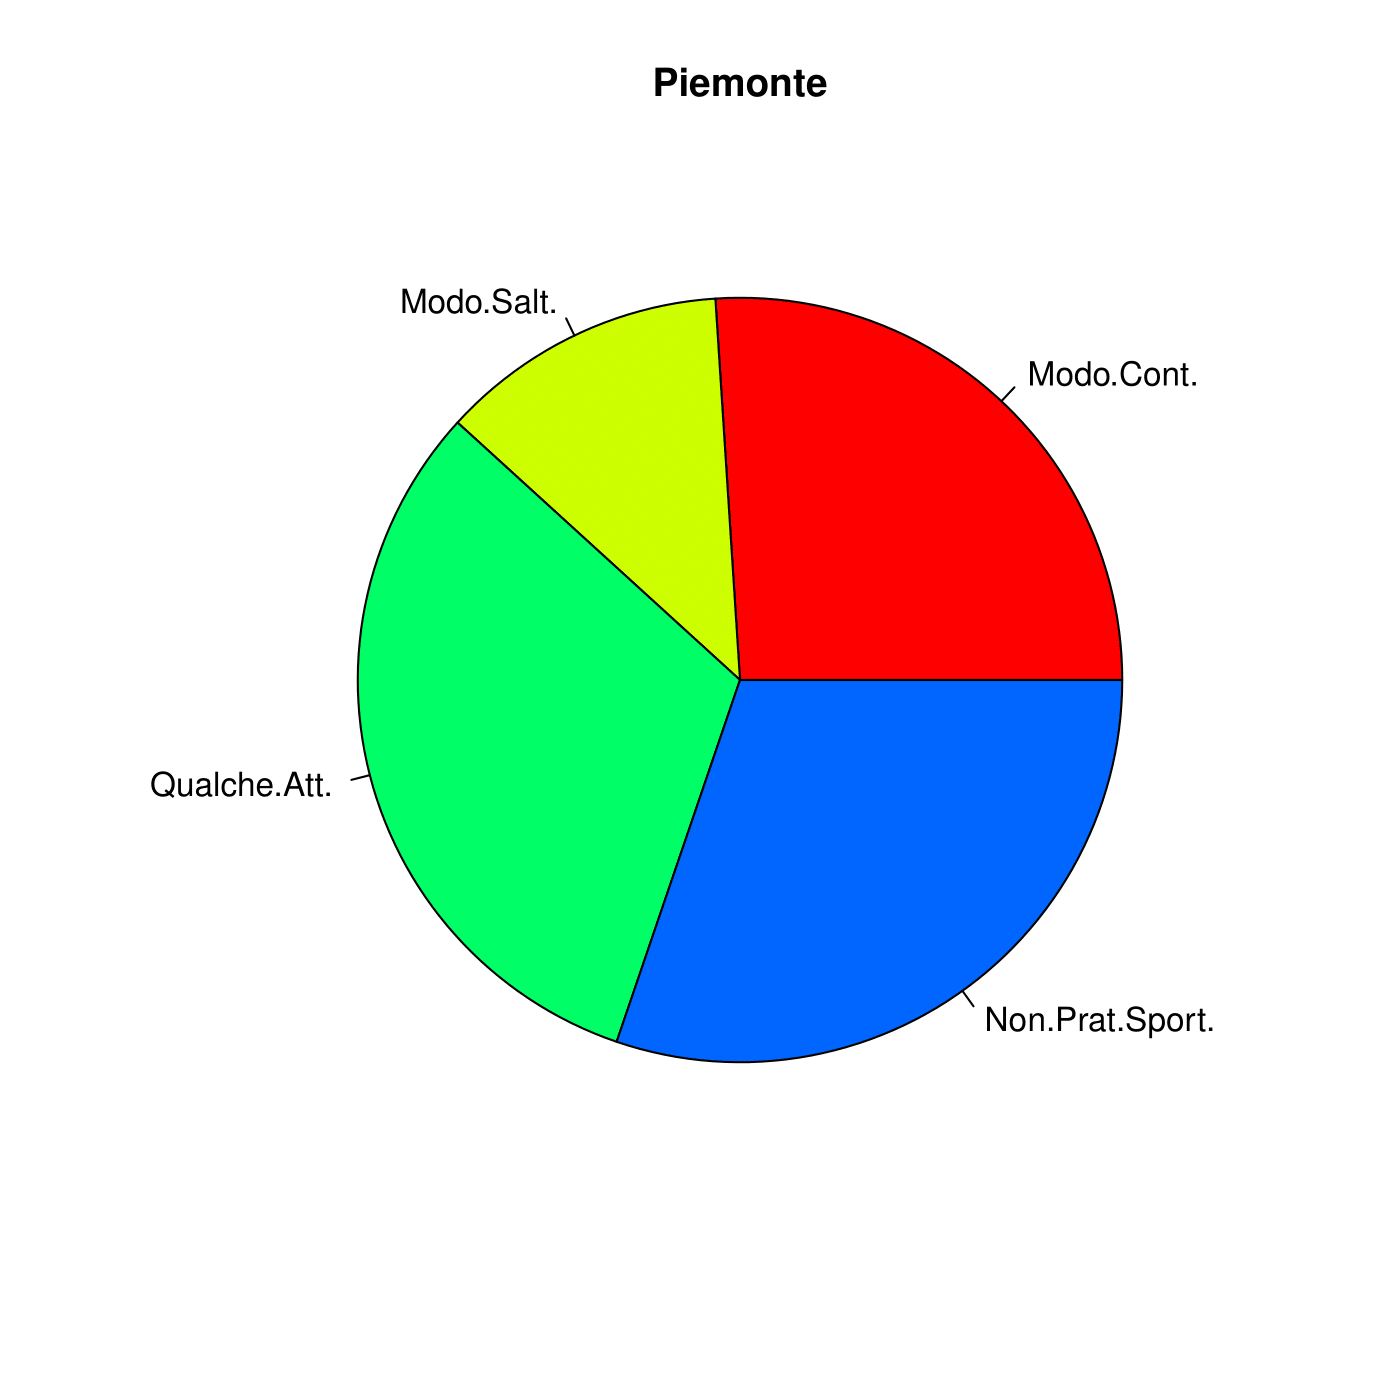
\includegraphics[height=8cm]{ProgettoSAD/capitoli/images/torta_regioni/torta_piemonte.png}}
        \qquad
        \subfloat{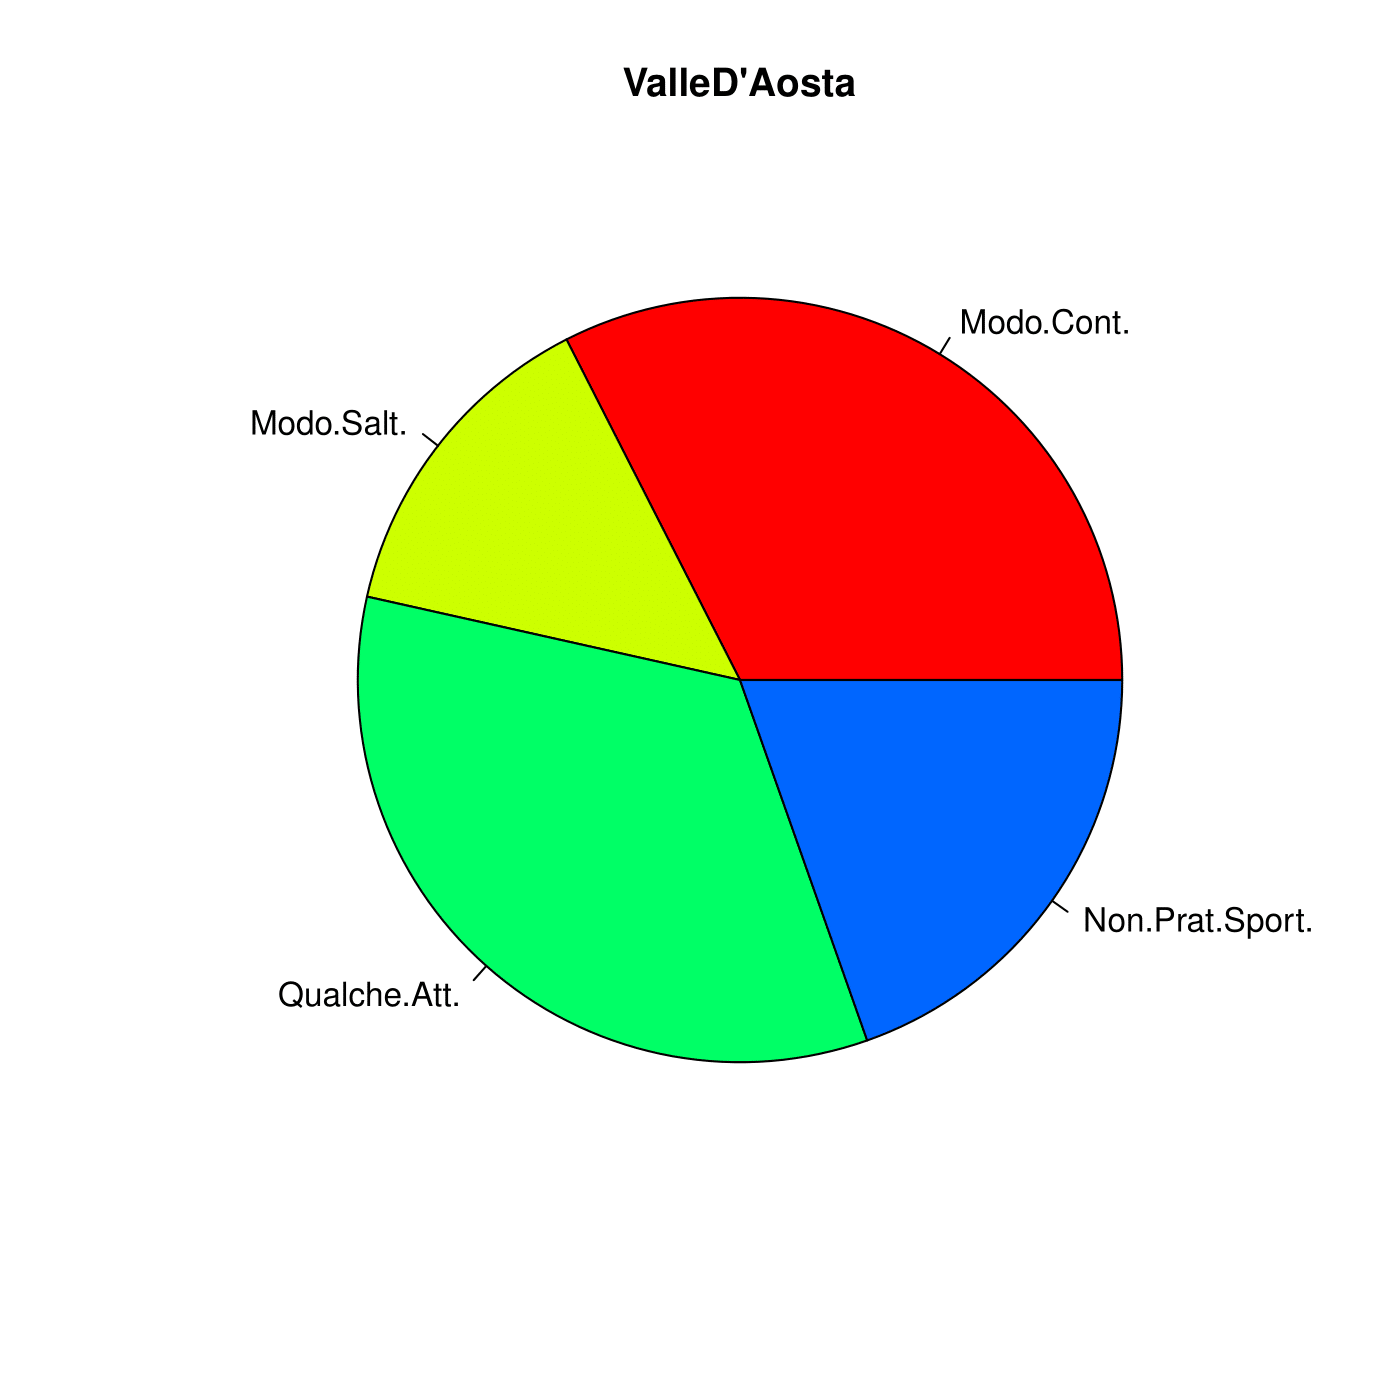
\includegraphics[height=8cm]{ProgettoSAD/capitoli/images/torta_regioni/torta_valledaosta.png}}
        \qquad
\end{figure}

\begin{figure}[!htbp]
    \centering
        \subfloat{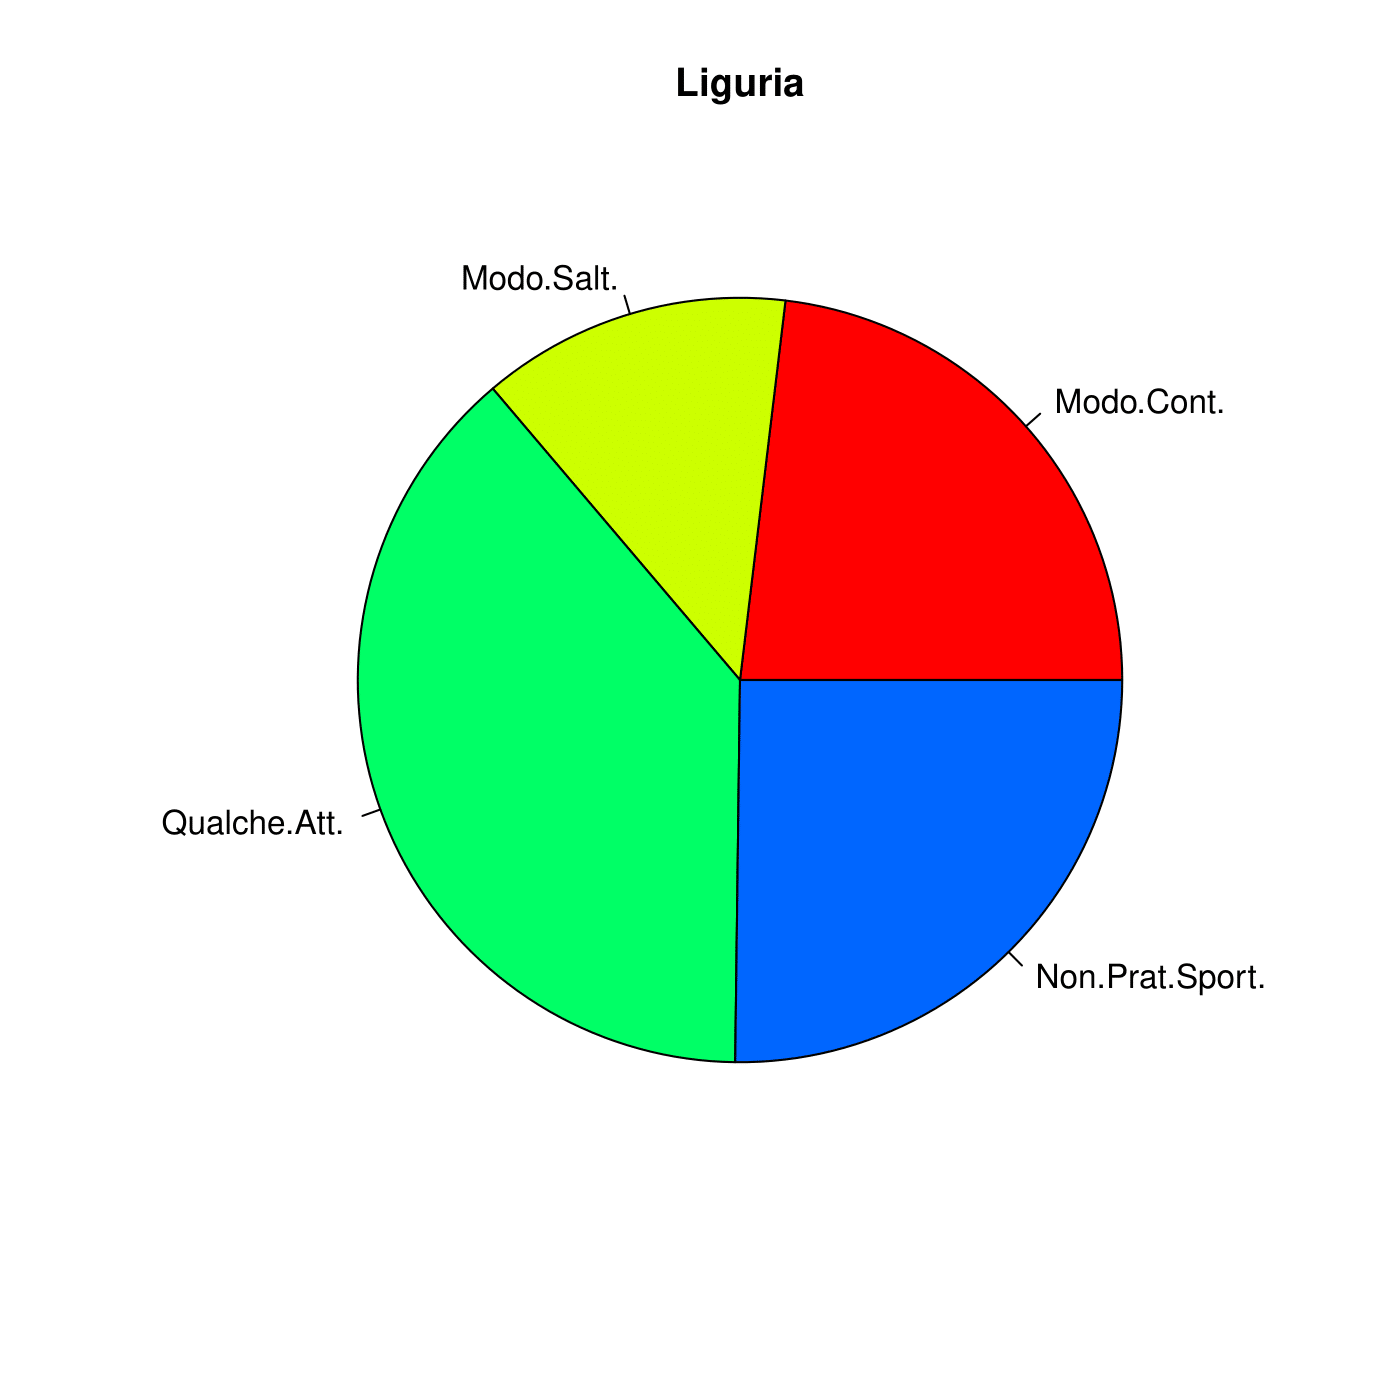
\includegraphics[height=8cm]{ProgettoSAD/capitoli/images/torta_regioni/torta_liguria.png}}
        \qquad
        \subfloat{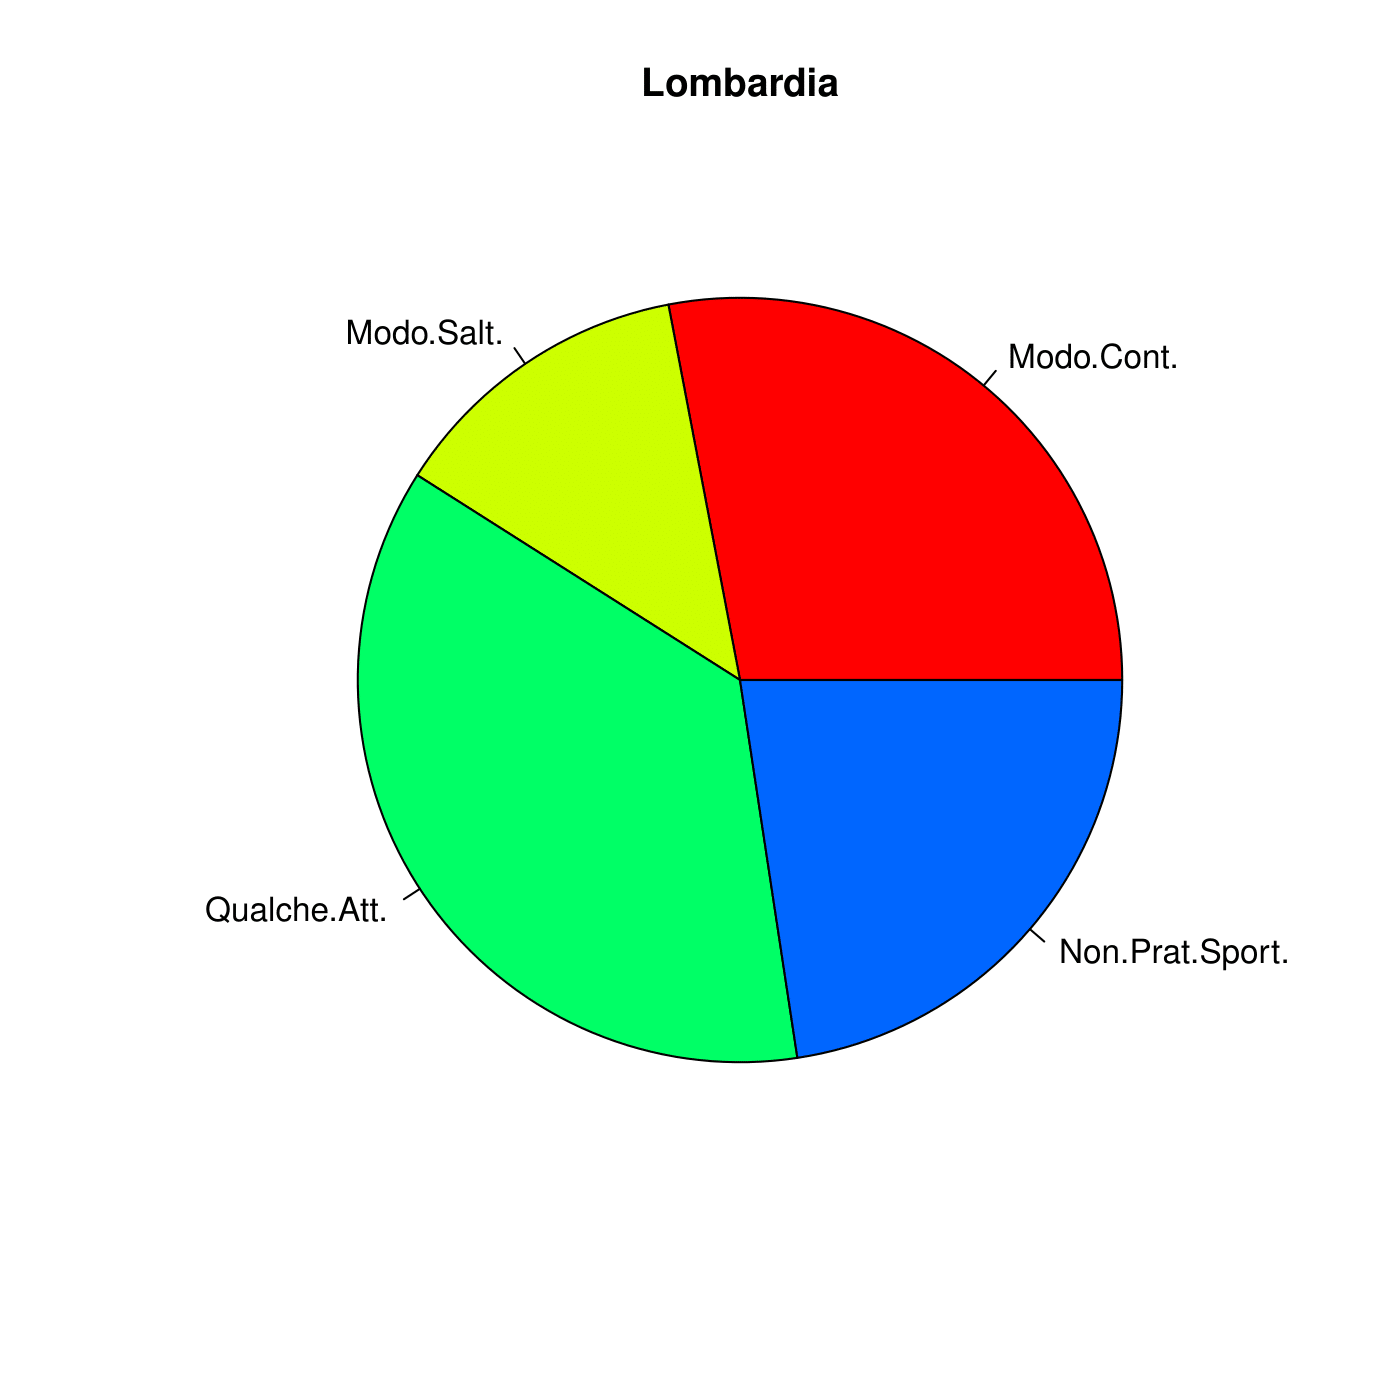
\includegraphics[height=8cm]{ProgettoSAD/capitoli/images/torta_regioni/torta_lombardia.png}}
        \qquad
\end{figure}
\begin{figure}[!htbp]
    \centering
        \subfloat{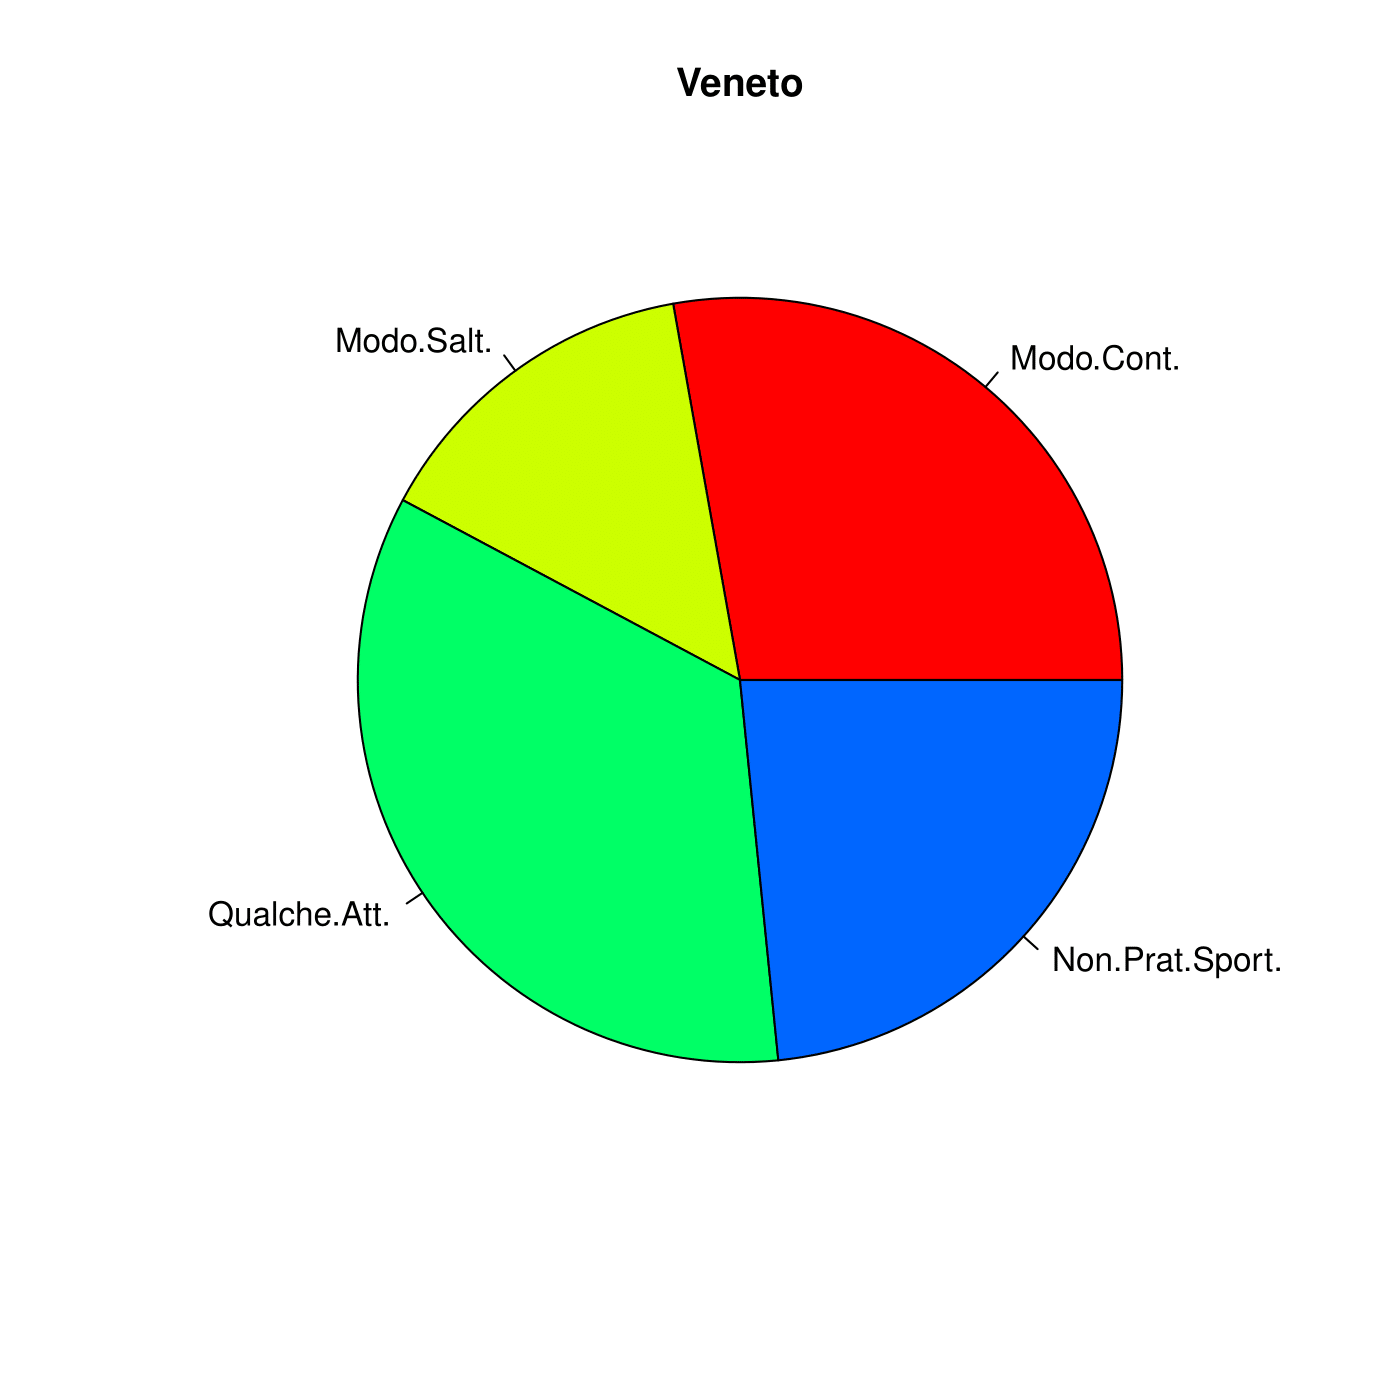
\includegraphics[height=8cm]{ProgettoSAD/capitoli/images/torta_regioni/torta_veneto.png}}
        \qquad
        \subfloat{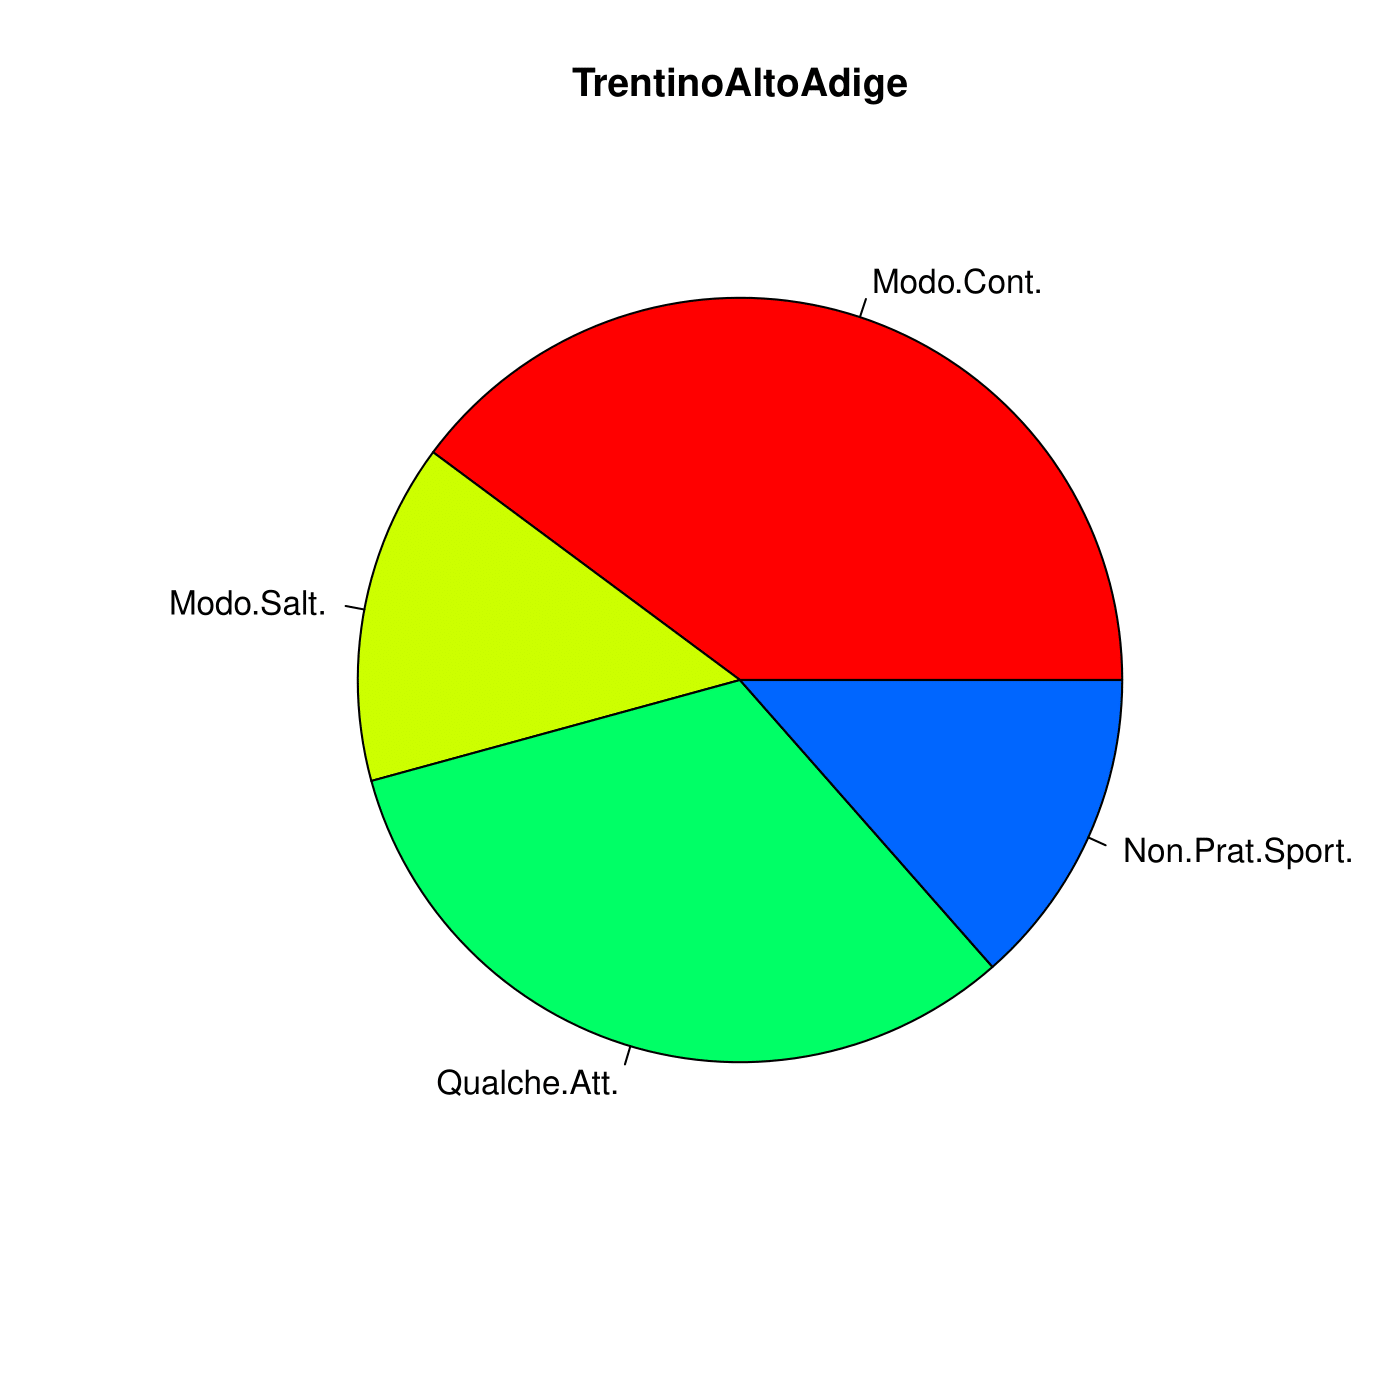
\includegraphics[height=8cm]{ProgettoSAD/capitoli/images/torta_regioni/trentino.png}}
        \qquad
\end{figure}
\begin{figure}[!htbp]
    \centering
        \subfloat{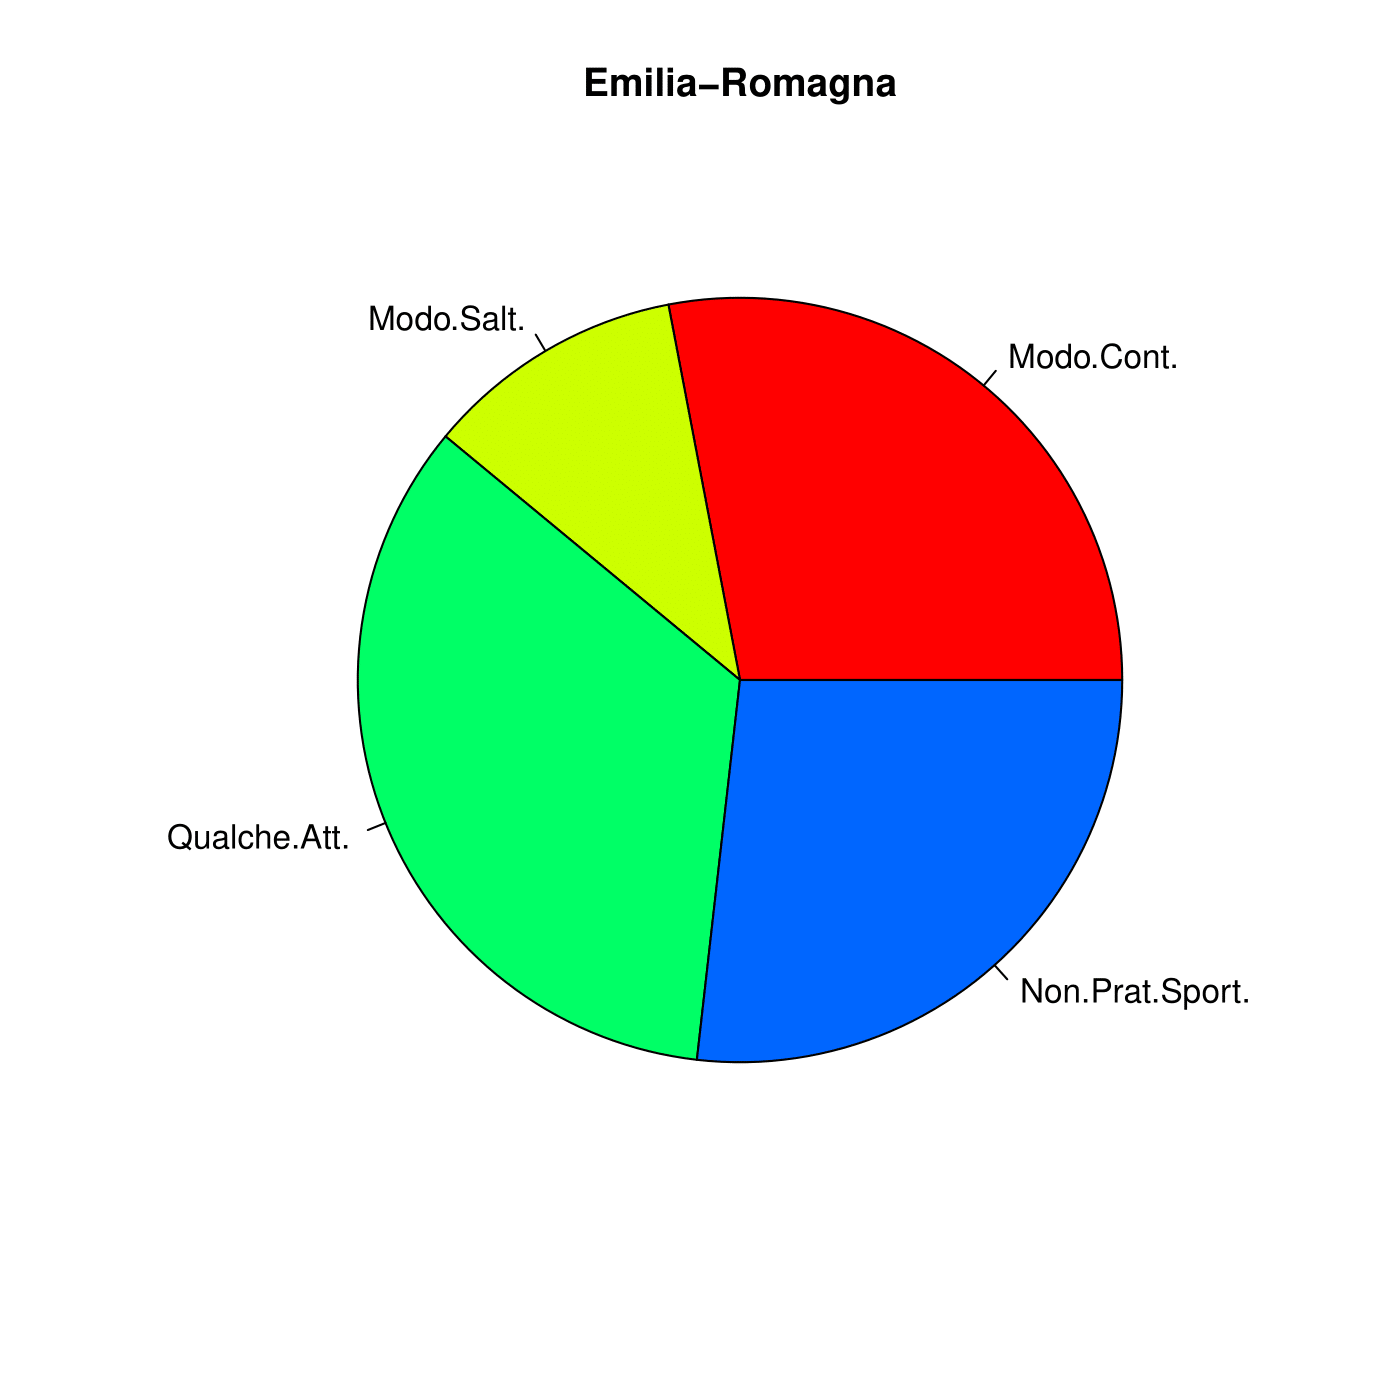
\includegraphics[height=8cm]{ProgettoSAD/capitoli/images/torta_regioni/torta_emilia.png}}
        \qquad
        \subfloat{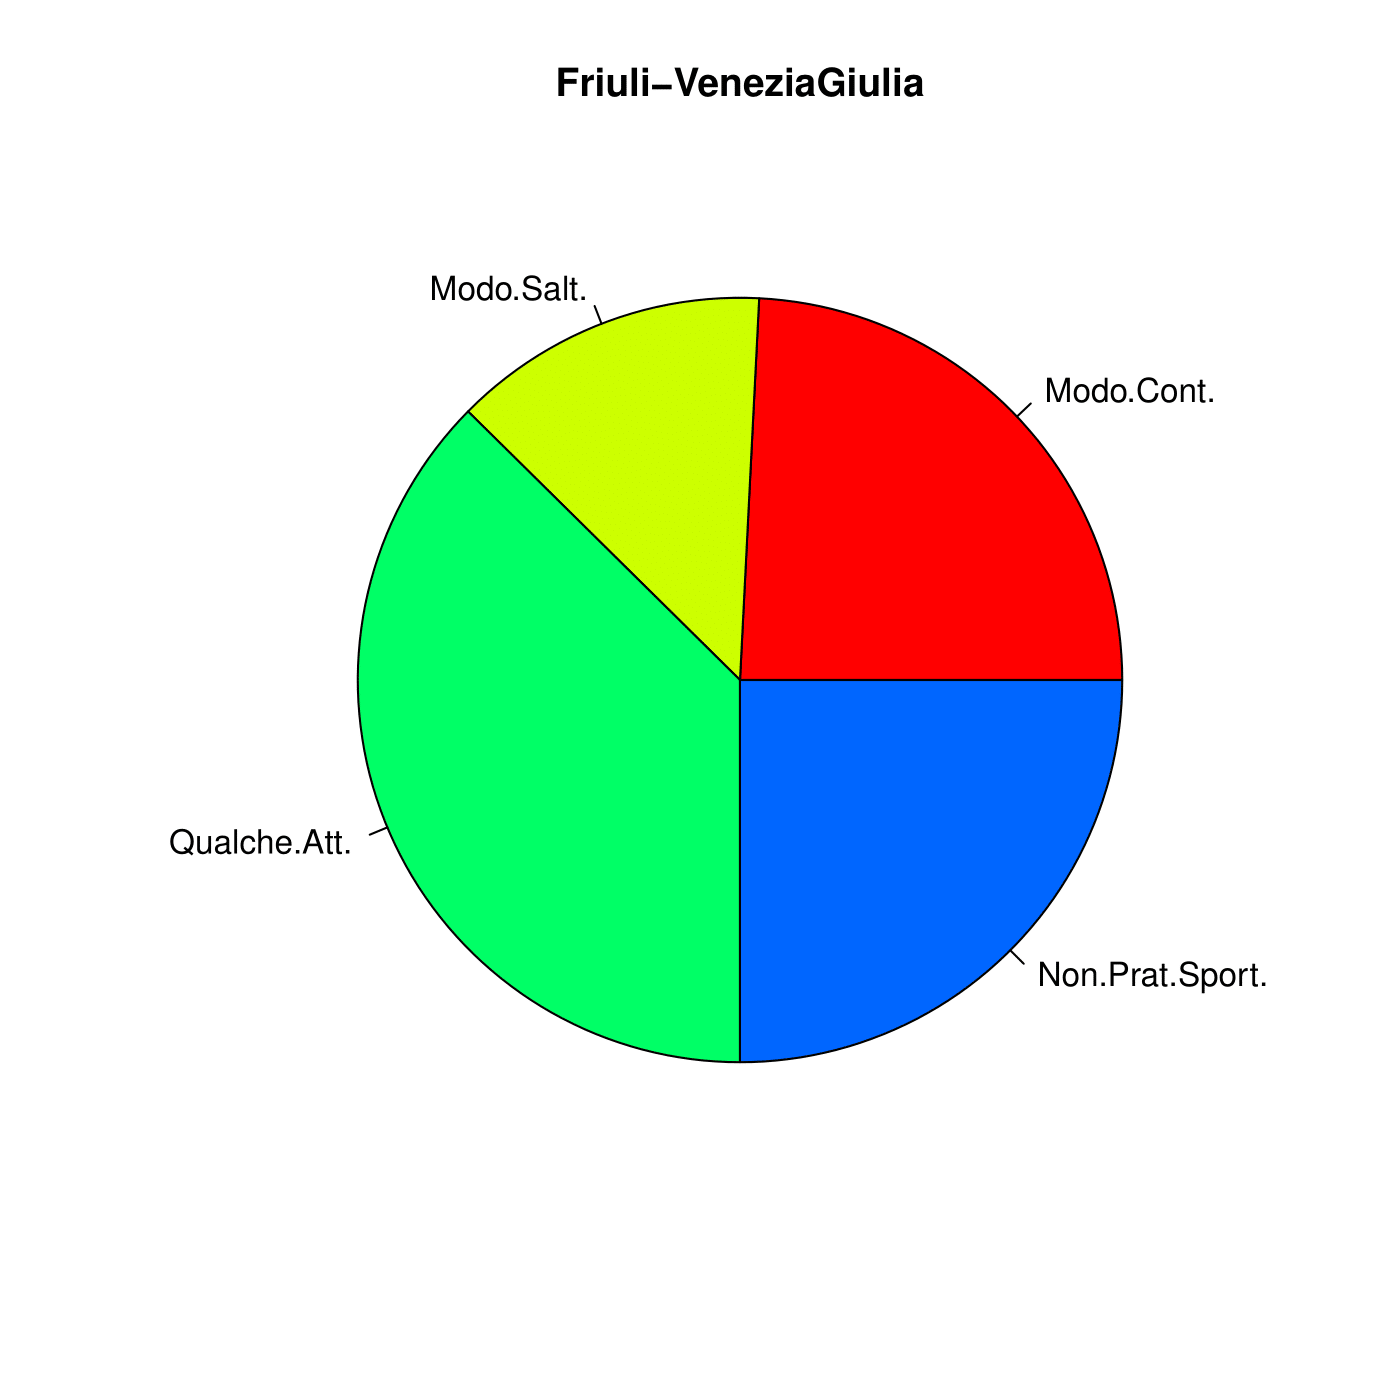
\includegraphics[height=8cm]{ProgettoSAD/capitoli/images/torta_regioni/torta_friuli.png}}
        \qquad
\end{figure}
\begin{figure}[!htbp]
    \centering
        \subfloat{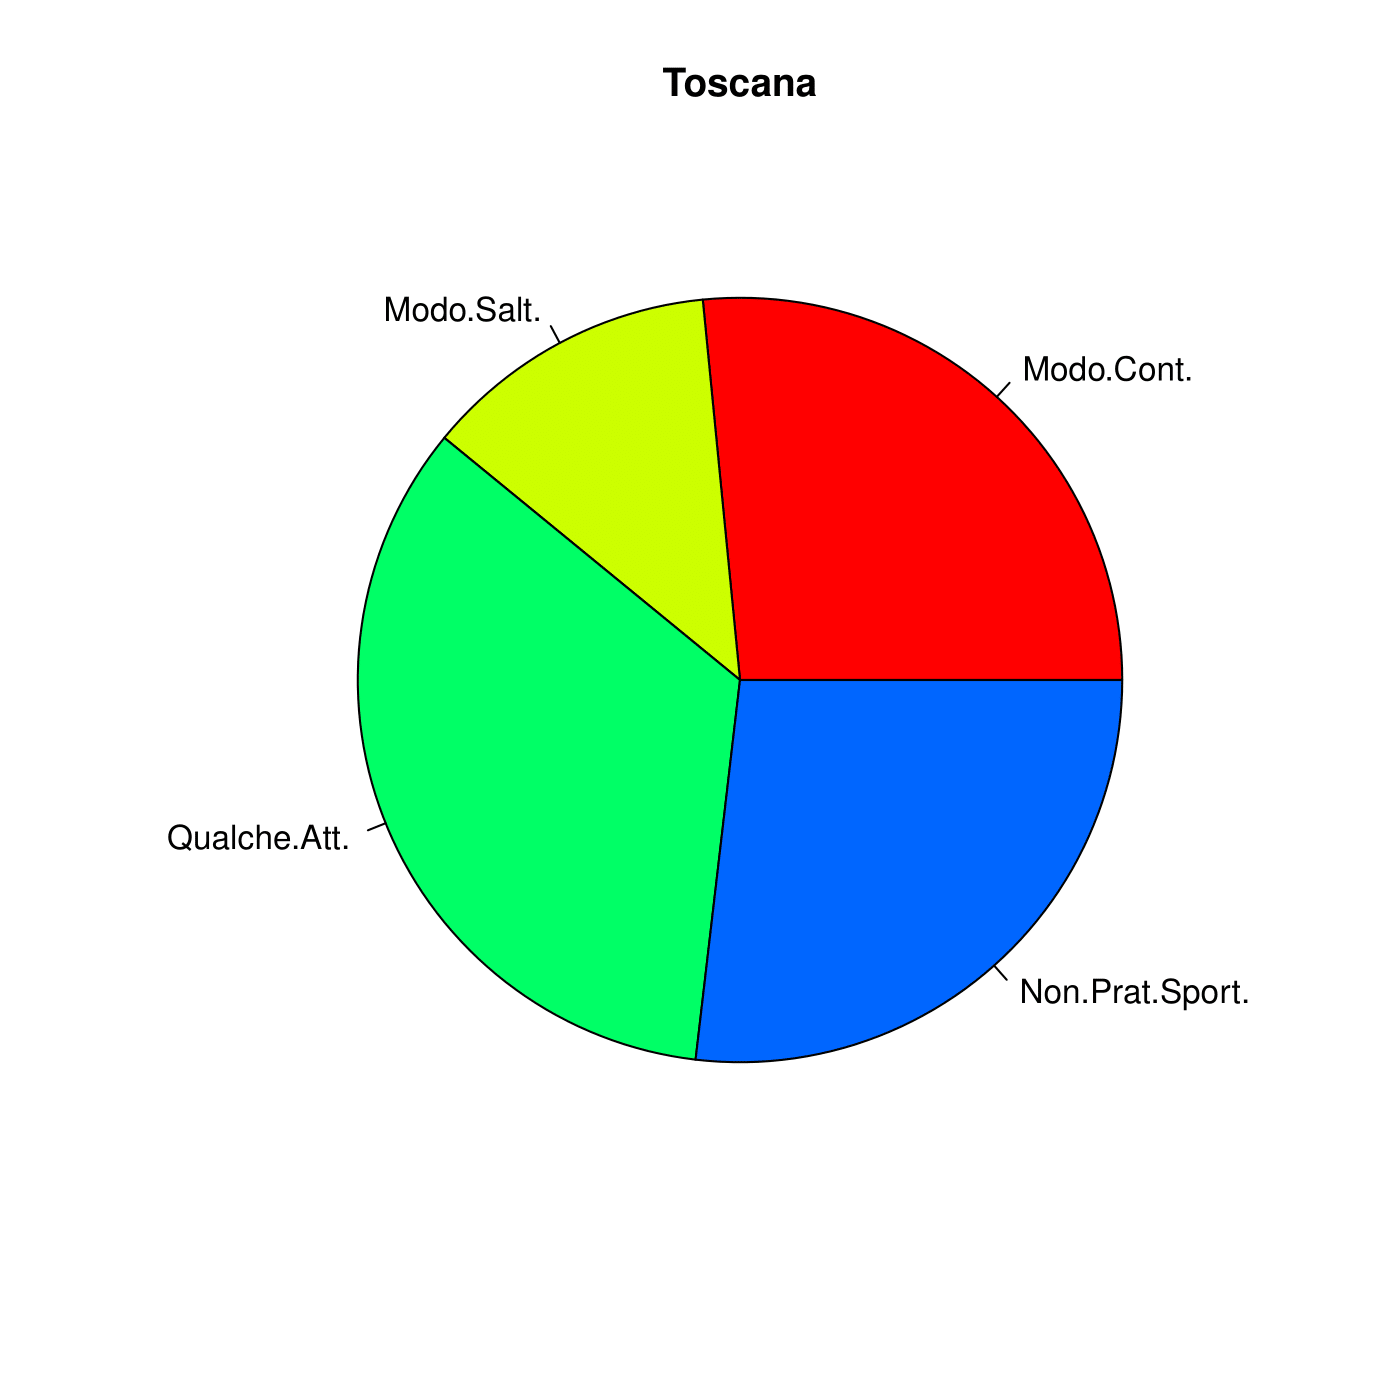
\includegraphics[height=8cm]{ProgettoSAD/capitoli/images/torta_regioni/torta_toscana.png}}
        \qquad
        \subfloat{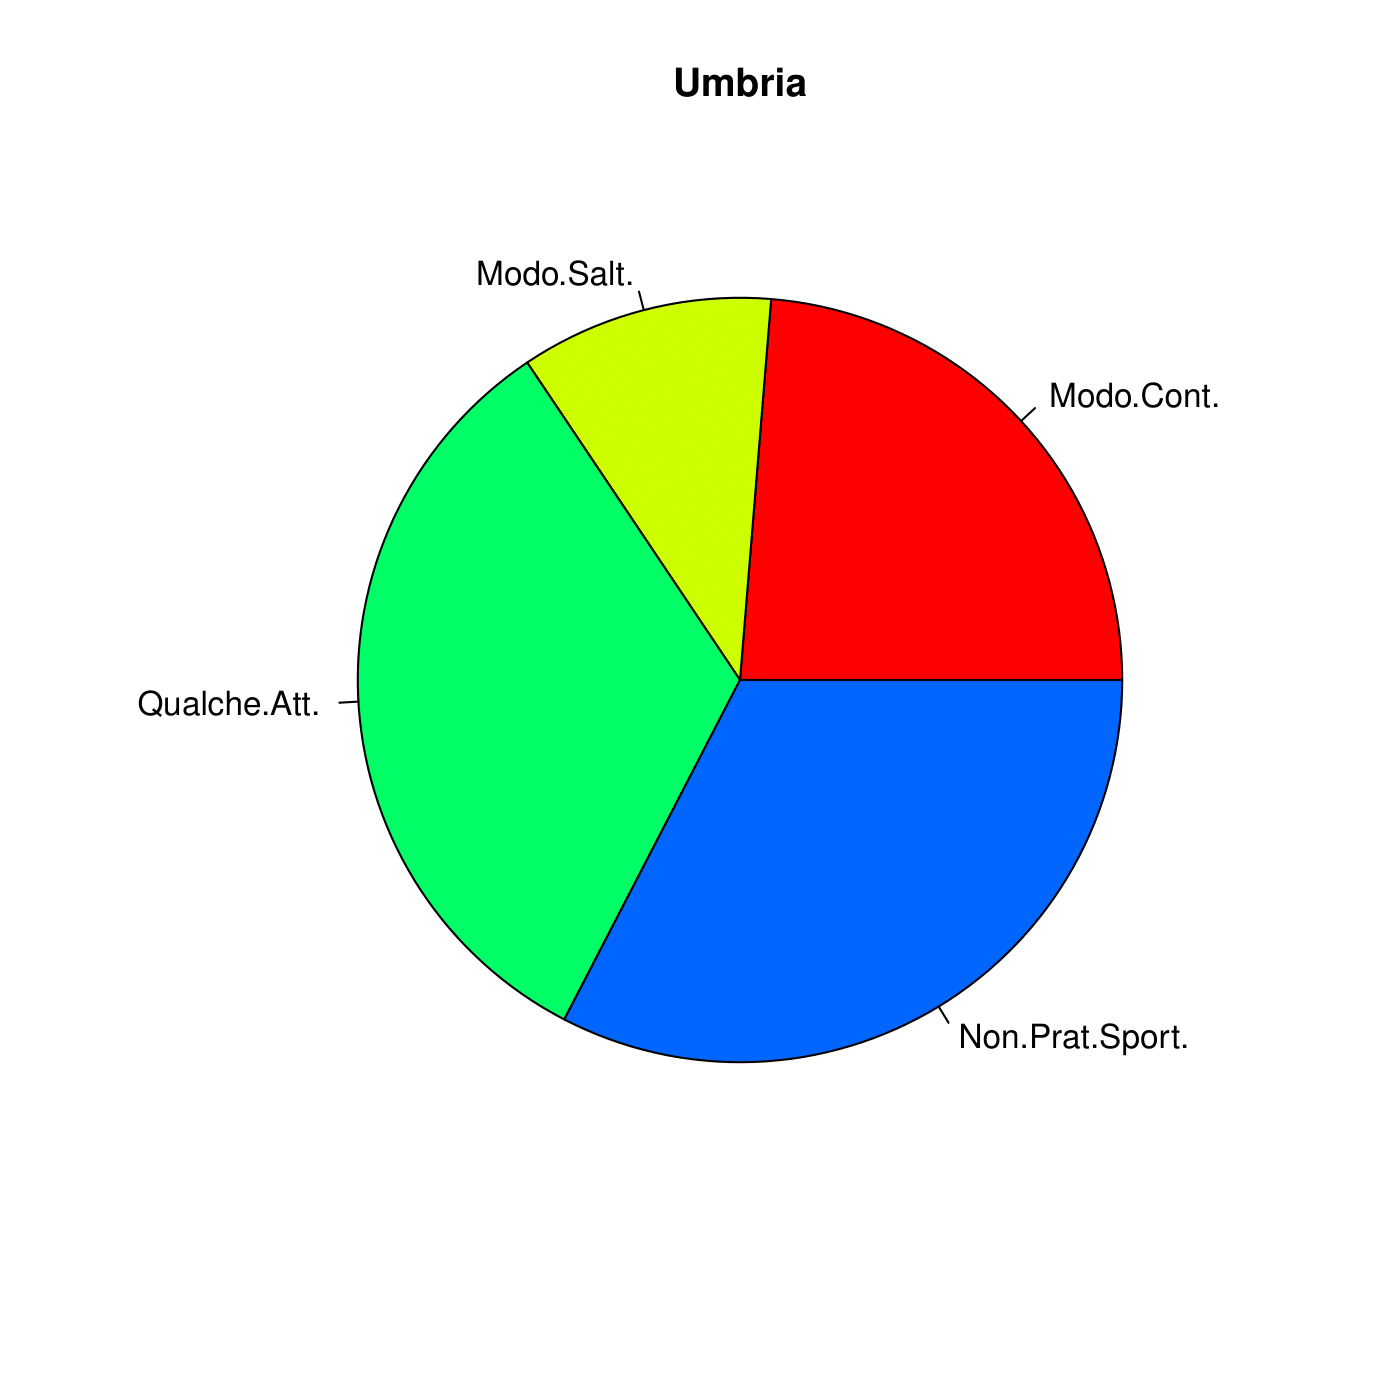
\includegraphics[height=8cm]{ProgettoSAD/capitoli/images/torta_regioni/torta_umbria.png}}
        \qquad
\end{figure}
\begin{figure}[!htbp]
    \centering
        \subfloat{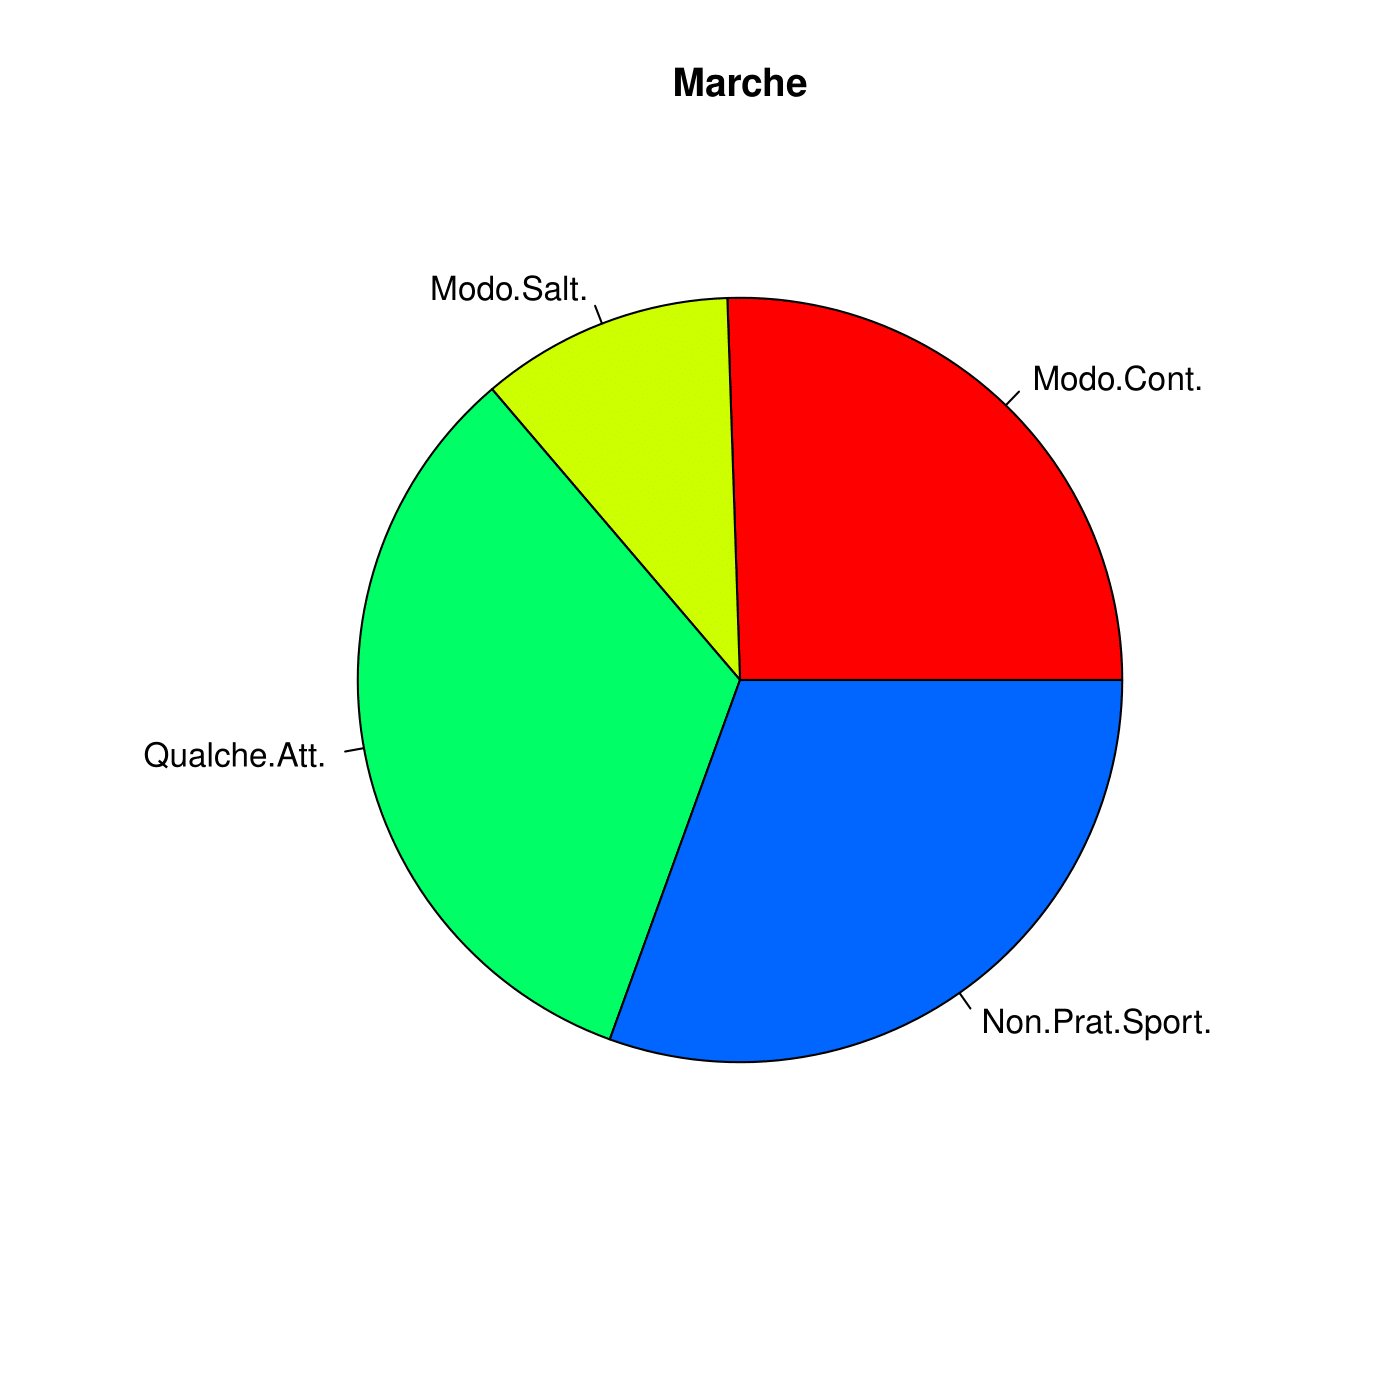
\includegraphics[height=8cm]{ProgettoSAD/capitoli/images/torta_regioni/torta_marche.png}}
        \qquad
        \subfloat{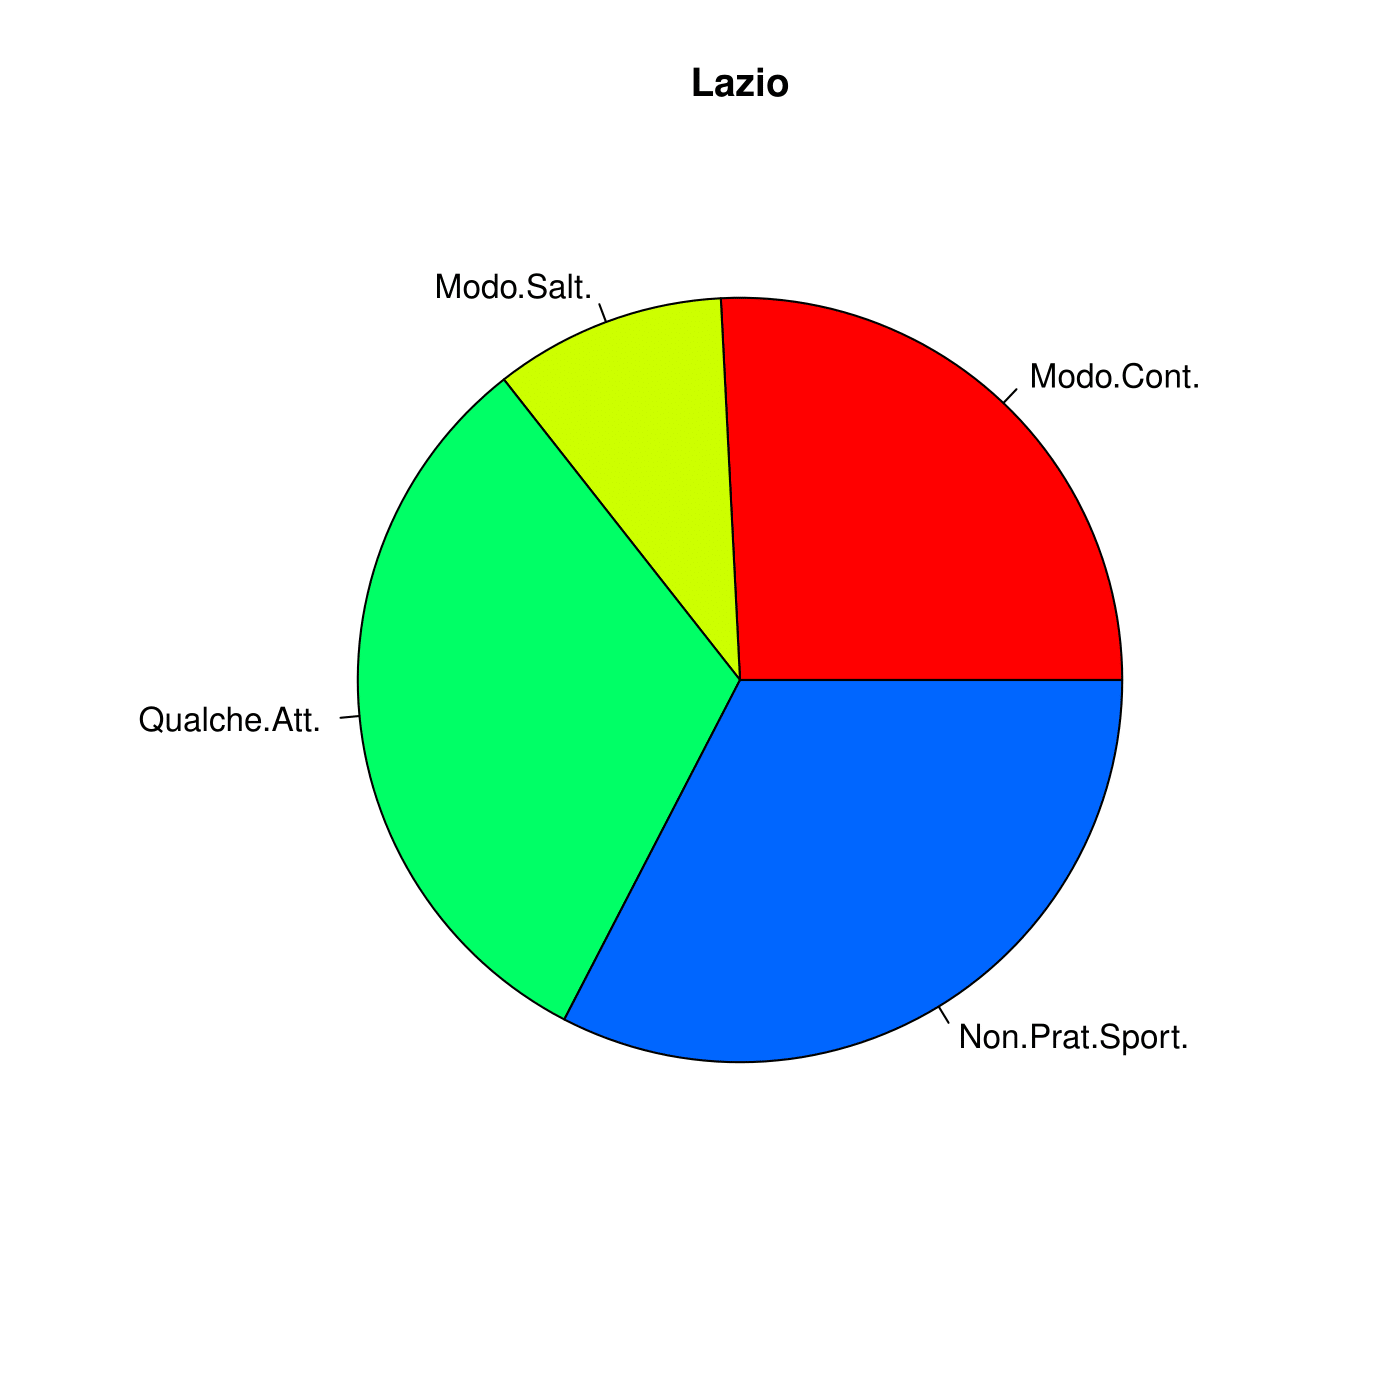
\includegraphics[height=8cm]{ProgettoSAD/capitoli/images/torta_regioni/torta_lazio.png}}
        \qquad
\end{figure}
\begin{figure}[!htbp]
    \centering
        \subfloat{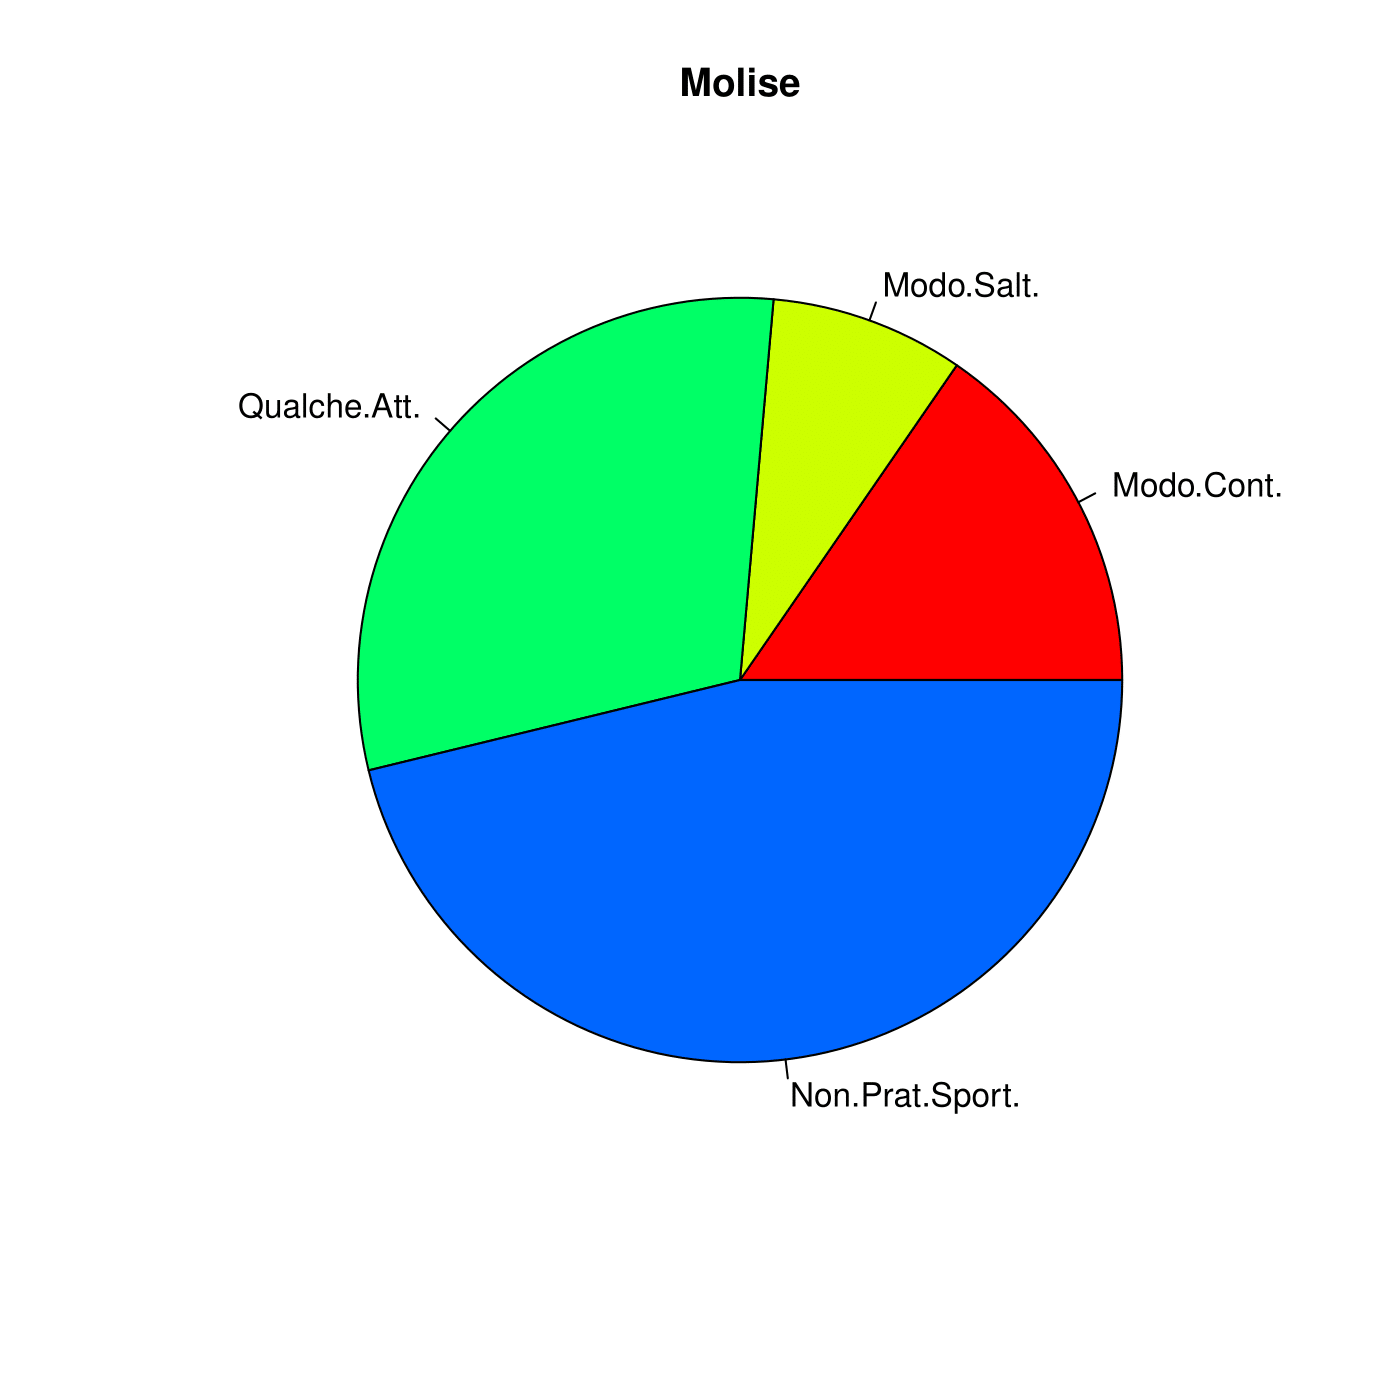
\includegraphics[height=8cm]{ProgettoSAD/capitoli/images/torta_regioni/torta_molise.png}}
        \qquad
        \subfloat{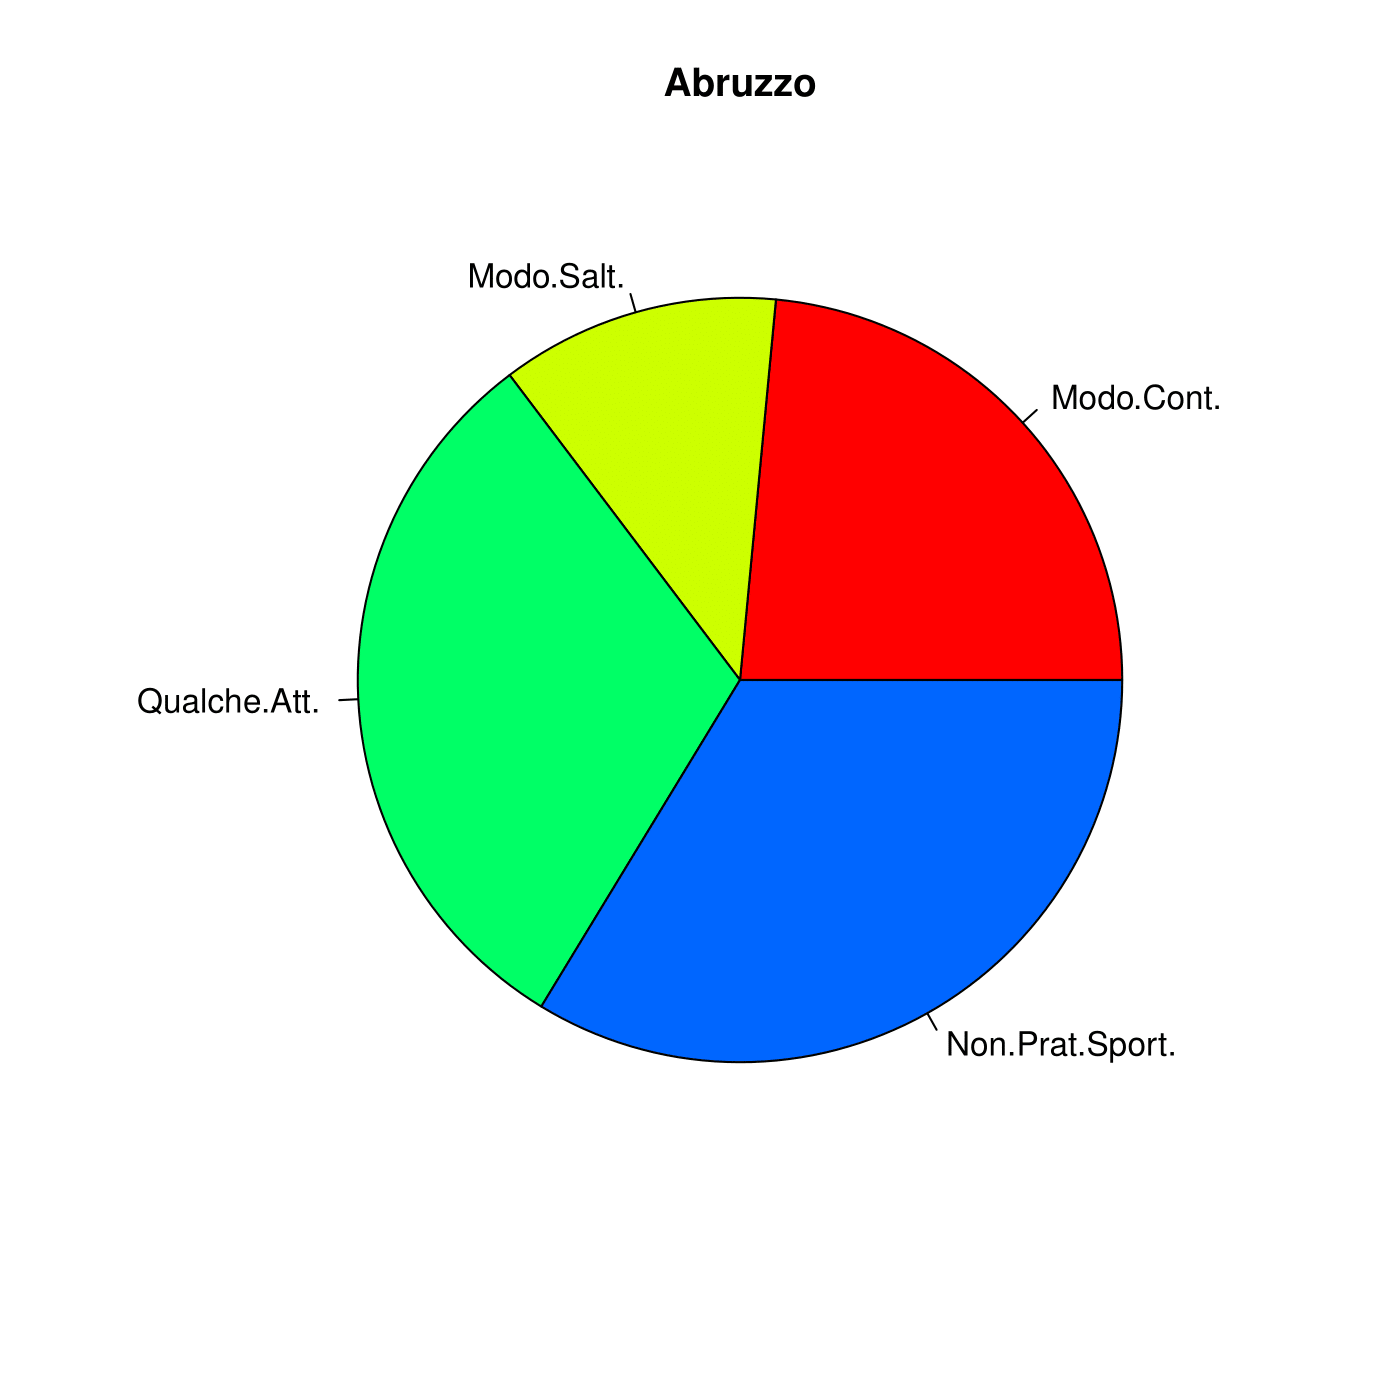
\includegraphics[height=8cm]{ProgettoSAD/capitoli/images/torta_regioni/torta_abruzzo.png}}
        \qquad
\end{figure}
\begin{figure}[!htbp]
    \centering
        \subfloat{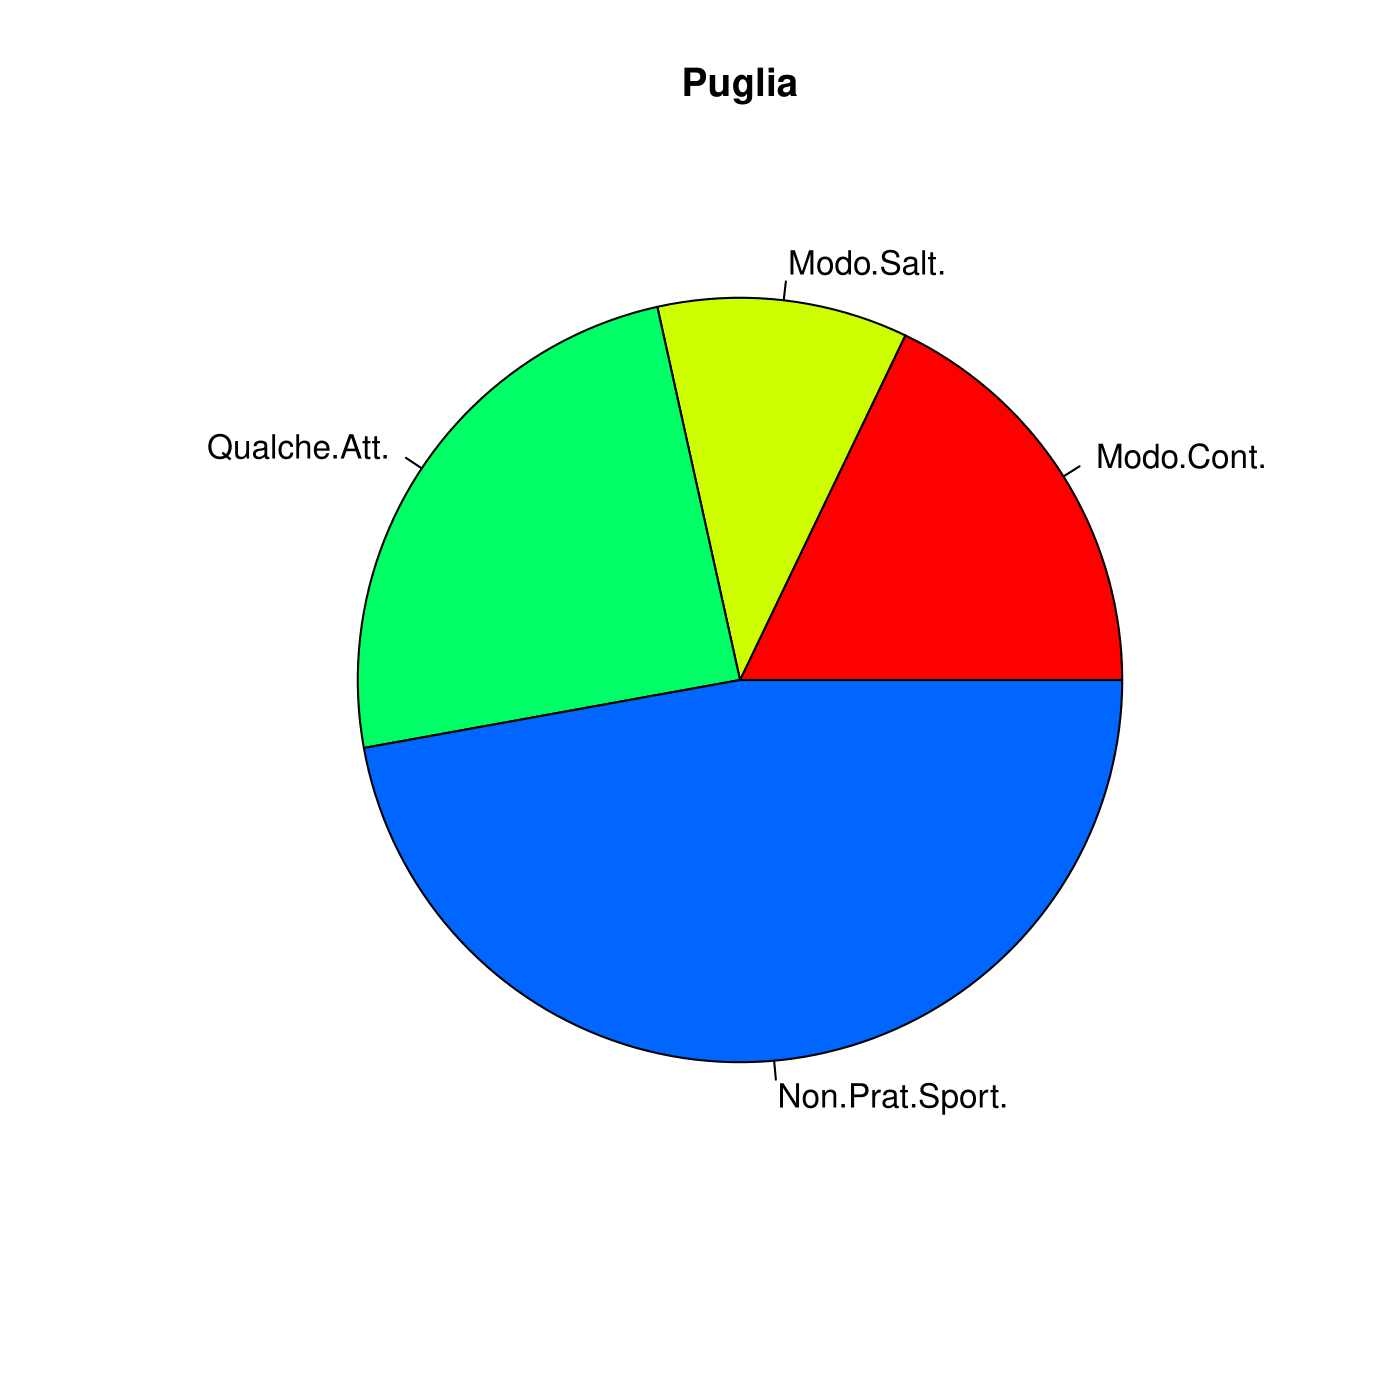
\includegraphics[height=8cm]{ProgettoSAD/capitoli/images/torta_regioni/torta_puglia.png}}
        \qquad
        \subfloat{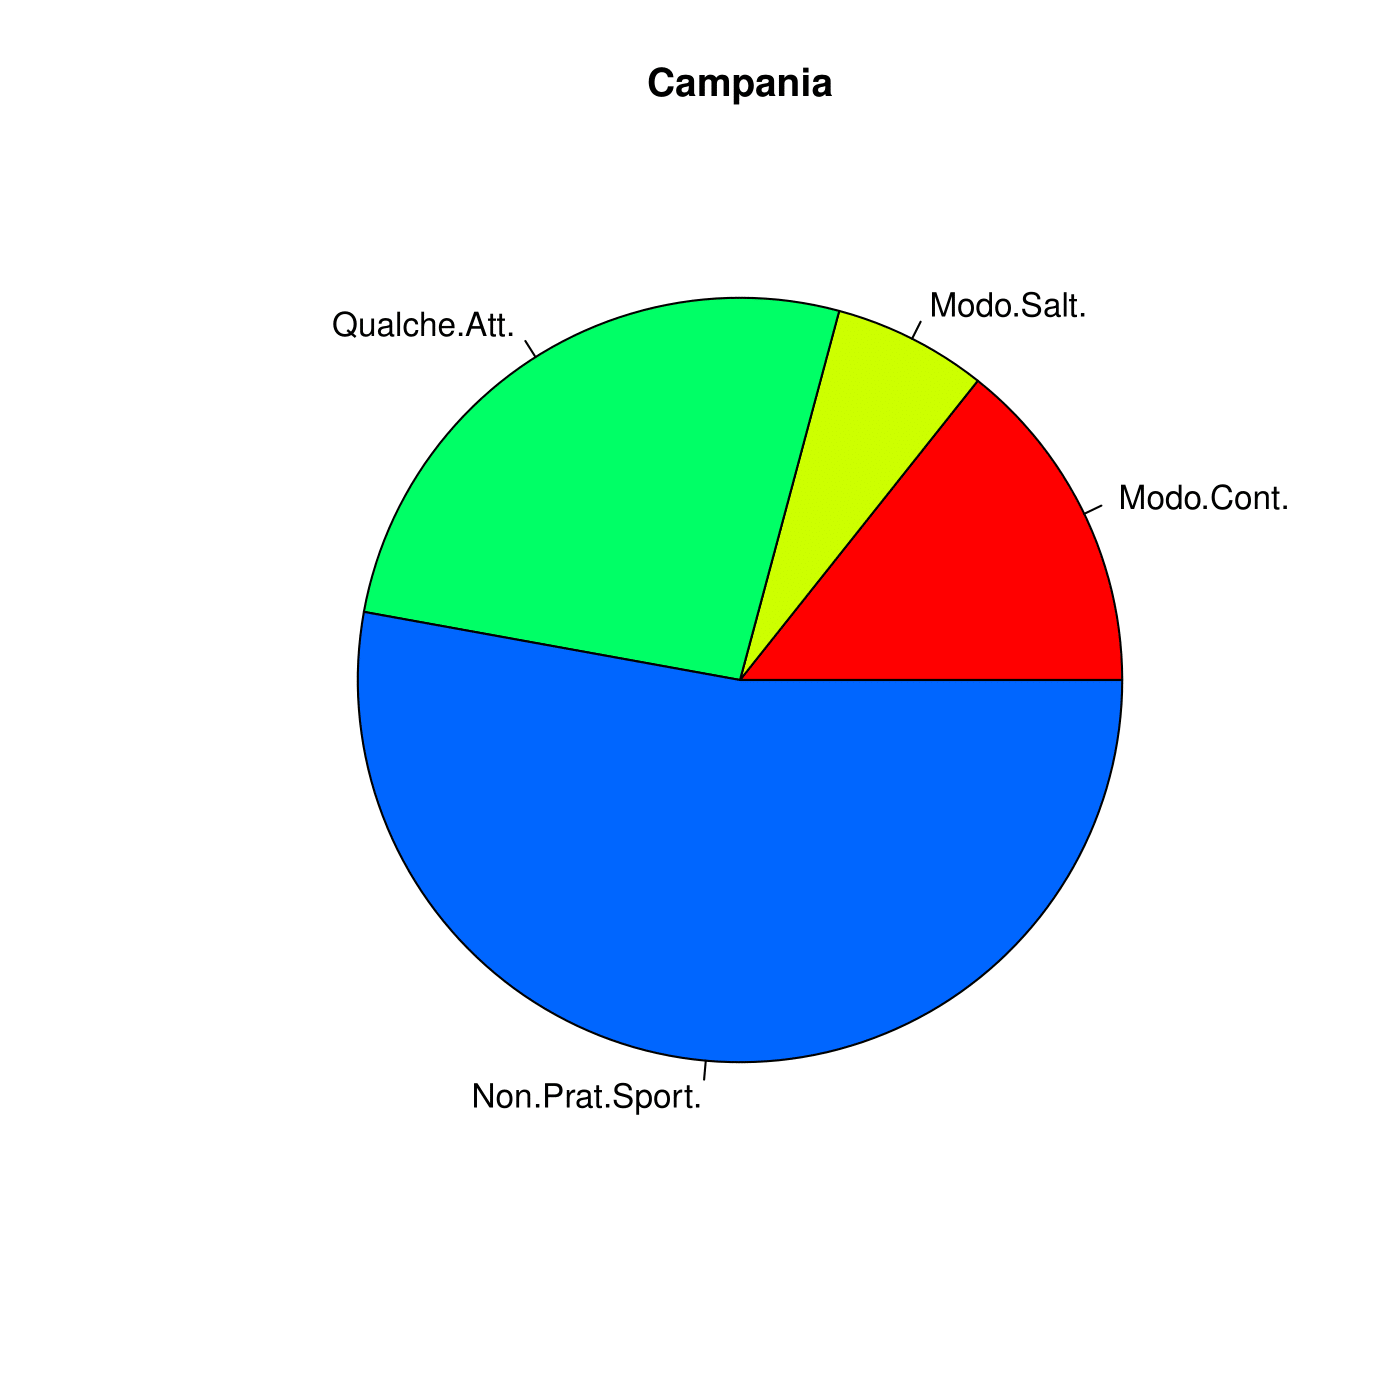
\includegraphics[height=8cm]{ProgettoSAD/capitoli/images/torta_regioni/torta_campania.png}}
        \qquad
\end{figure}
\begin{figure}[!htbp]
    \centering
        \subfloat{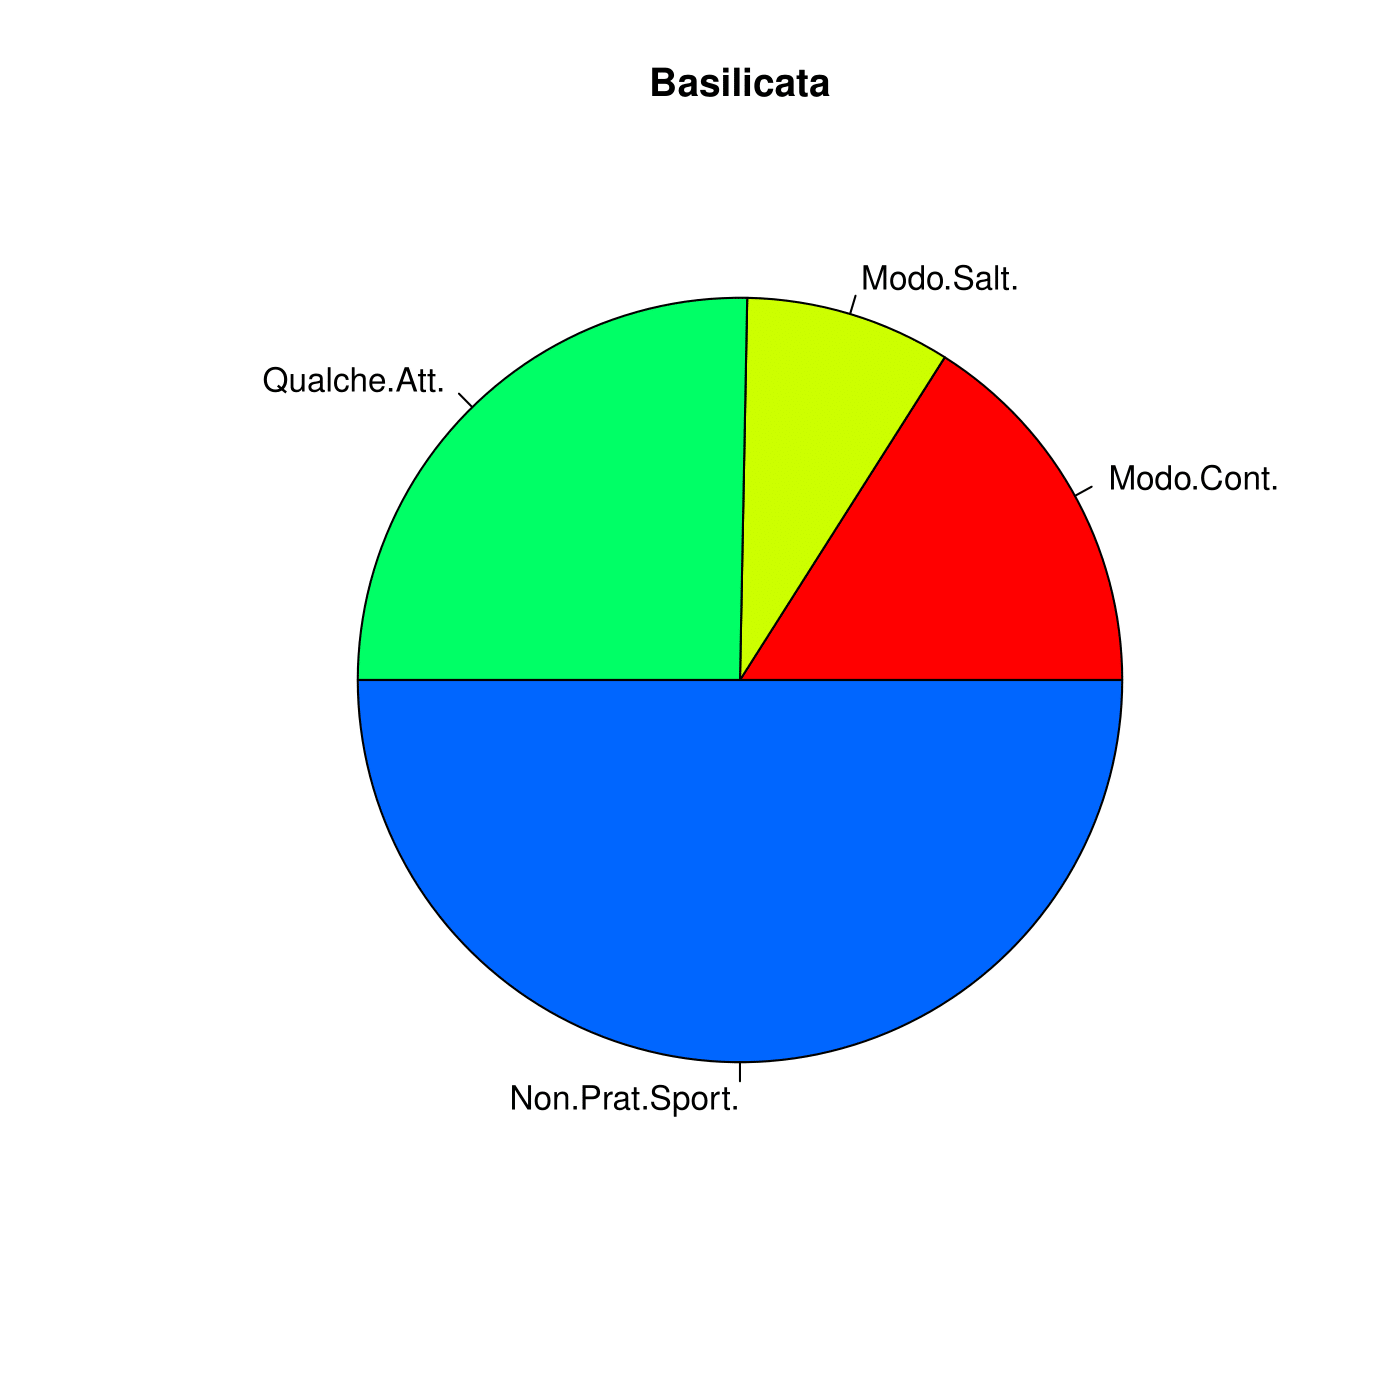
\includegraphics[height=8cm]{ProgettoSAD/capitoli/images/torta_regioni/torta_basilicata.png}}
        \qquad
        \subfloat{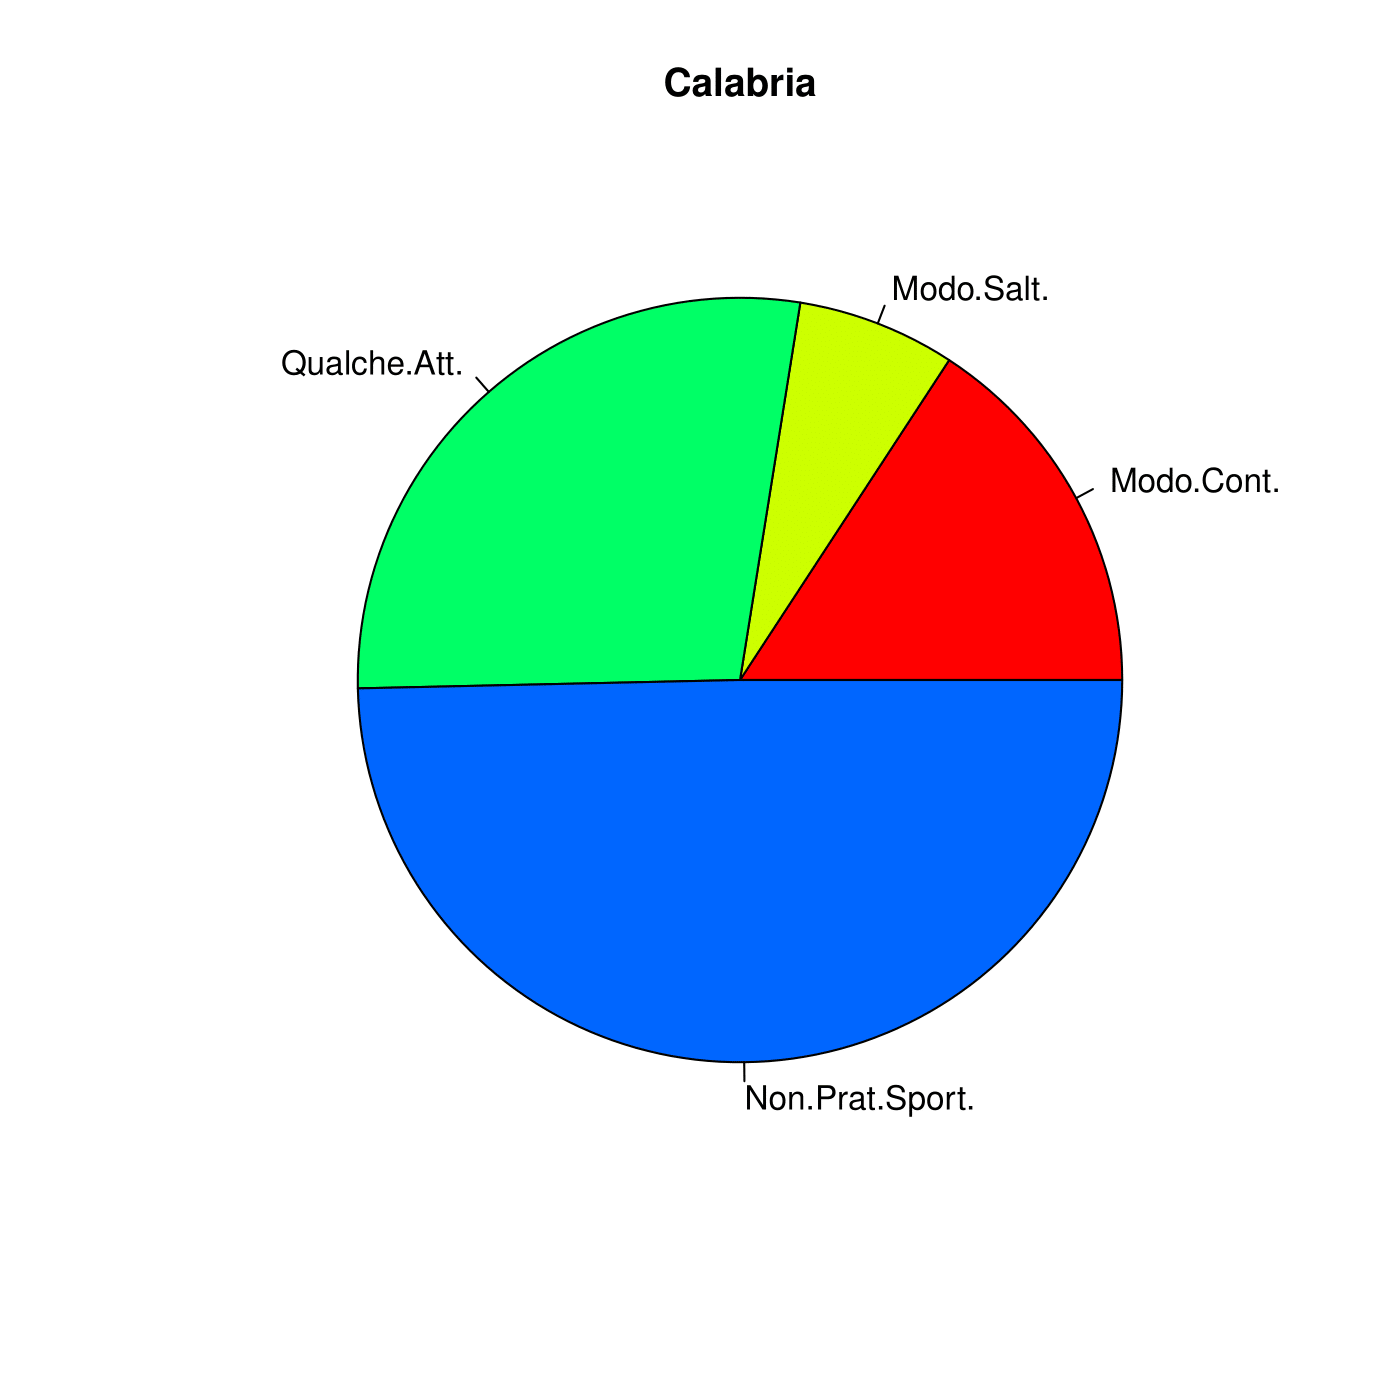
\includegraphics[height=8cm]{ProgettoSAD/capitoli/images/torta_regioni/torta_calabria.png}}
        \qquad
\end{figure}
\begin{figure}[!htbp]
    \centering
        \subfloat{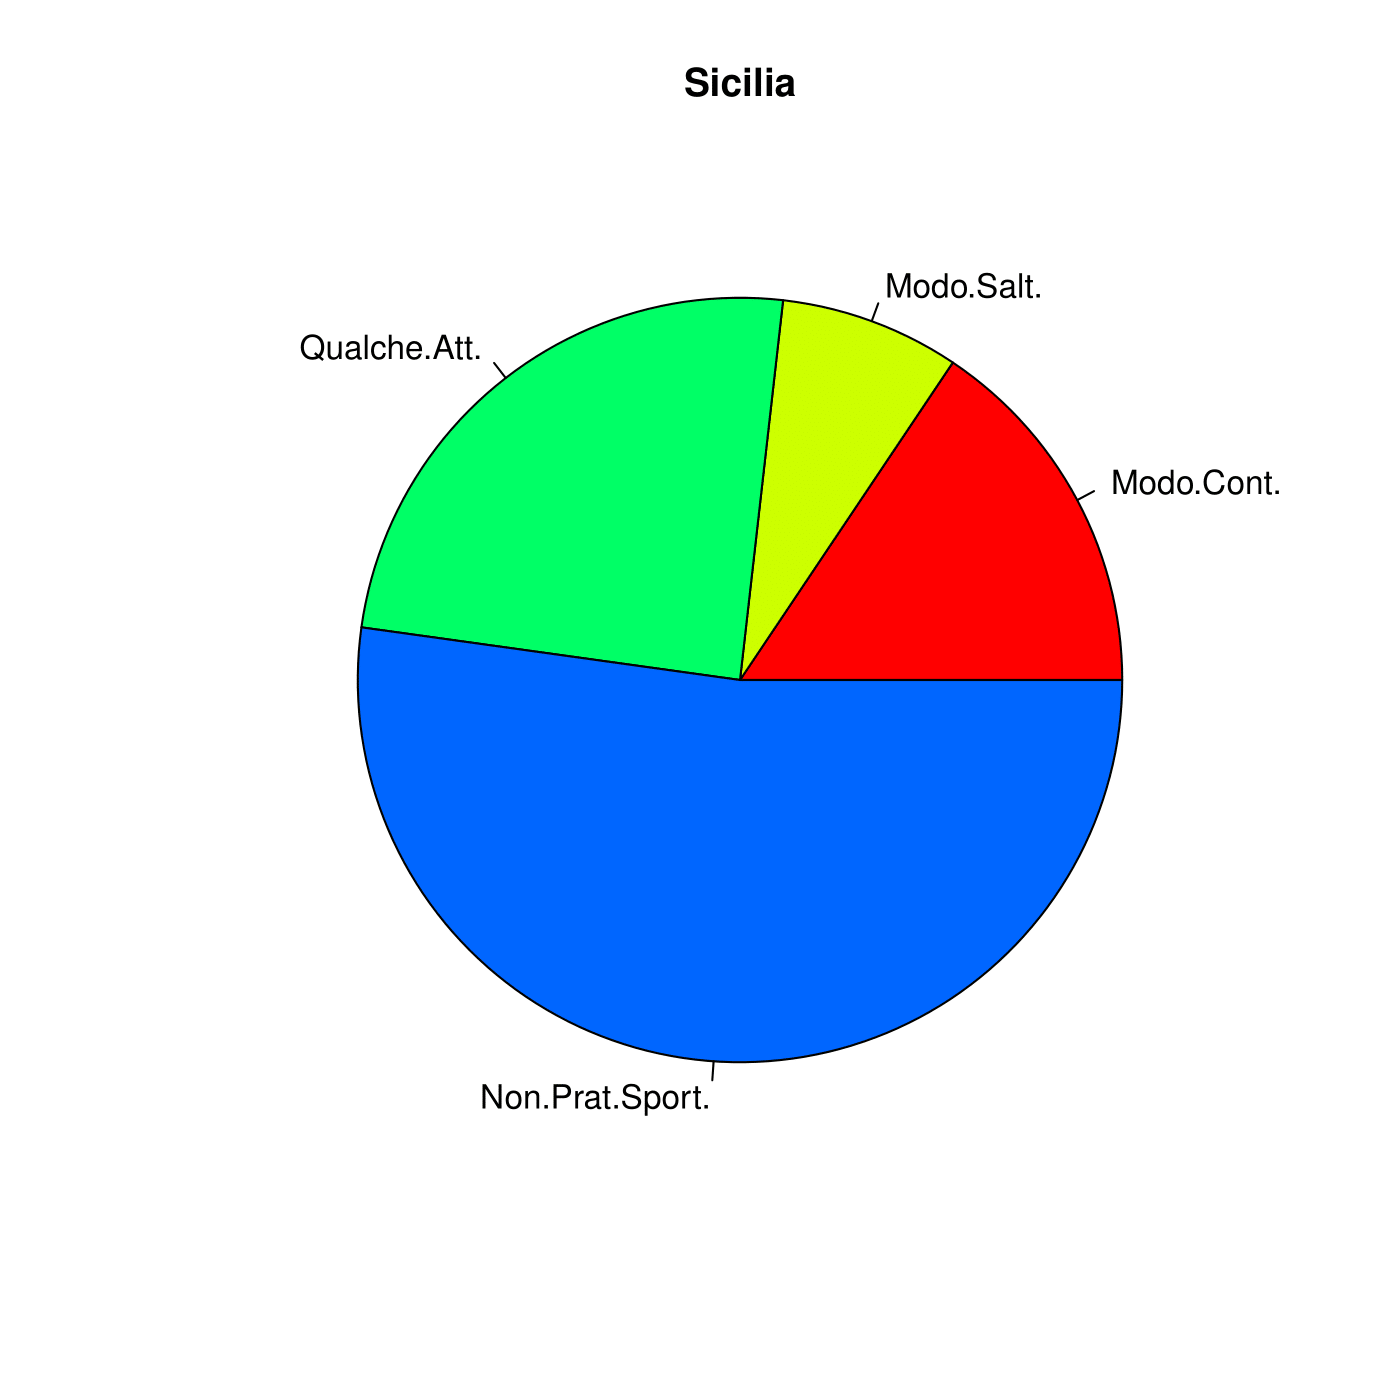
\includegraphics[height=8cm]{ProgettoSAD/capitoli/images/torta_regioni/torta_sicilia.png}}
        \qquad
        \subfloat{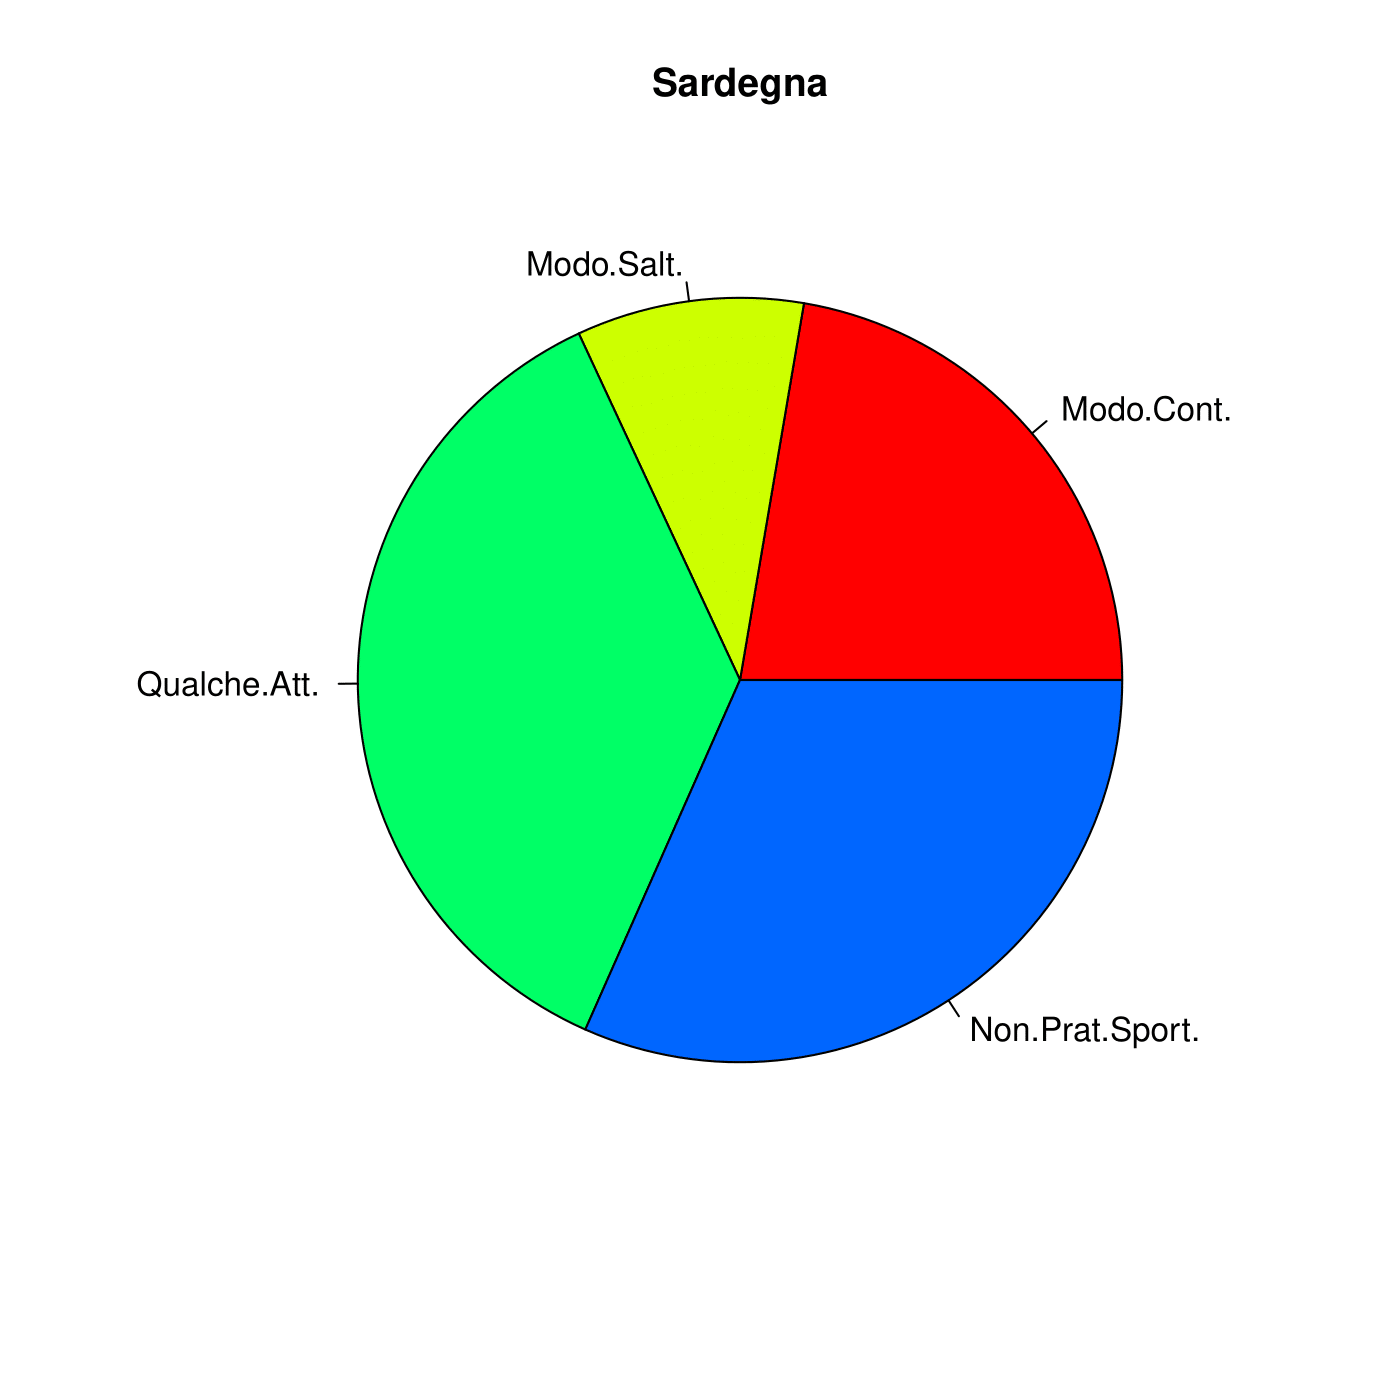
\includegraphics[height=8cm]{ProgettoSAD/capitoli/images/torta_regioni/torta_sardegna.png}}
        \qquad
\end{figure}

Dai grafici a torta disegnati possiamo trarre le stesse conclusioni ottenute 
per i grafici a barre rispetto le caratteristiche.

%################################################

\newpage
\phantomsection
\definecolor{dkgreen}{rgb}{0,0.6,0}
\definecolor{gray}{rgb}{0.5,0.5,0.5}
\definecolor{mauve}{rgb}{0.58,0,0.82}


\lstset{frame=tb,
language=R,
aboveskip=3mm,
belowskip=3mm,
showstringspaces=false,
columns=flexible,
numbers=none,
inputencoding=utf8/latin1,
keywordstyle=\color{blue},
numberstyle=\tiny\color{gray},
commentstyle=\color{dkgreen},
stringstyle=\color{mauve},
breaklines=true,
breakatwhitespace=true,
tabsize=3
}

\chapter{Statistica Descrittiva Univariata}\label{cap3}

In questo capitolo e nel prossimo si svilupperà la statistica descrittiva, ossia il ramo della statistica che si occupa dei metodi di analisi e di sintesi dei dati. La statistica descrittiva è utilizzata per analizzare il comportamento dei fenomeni oggetti di studio, attraverso metodi di natura logica e matematica. Ogni fenomeno può essere descritto tramite opportune categorie di dati di tipo qualitativo oppure di tipo quantitativo discreti o continui. I dati sono utilizzati per ricavare \textit{misure di sintesi} che consentano di comprendere il comportamento del fenomeno in esame. Sulla base dell'analisi dei dati è spesso possibile formulare opportune ipotesi statistiche da sottoporre successivamente a procedimenti di verifica mediante gli strumenti tipici dell'inferenza statistica.

Alcuni \textbf{indici di sintesi} (detti anche statistiche), utili a descrivere dei dati numerici, sono \textit{media, mediana, moda, varianza, deviazione standard} e \textit{coefficiente di variazione}. La media e la mediana sono misure di \textit{centralità}, mentre la varianza e la deviazione standard misurano la \textit{dispersione} dei dati.

\section{Indici di sintesi: Misure di centralità}\label{cap3.1}

In questa sezione ci occuperemo delle misure di centralità: media e mediana.

\subsection{Media Campionaria}\label{cap3.1.1}

Dato un campione \textit{$x_1, x_2,...,x_n$} di ampiezza \textit{n}, dove \textit{n} indica il numero di dati statistici numerici, la \textit{media campionaria} risulta essere la media aritmetica degli \textit{n} valori.

\noindent \textbf{Definizione:} Si definisce \textbf{\textit{media campionaria}} e si denota con $\Bar{x}$ la quantità:

\[\overline{x} = \frac{1}{n} \sum_{i=1}^n x_i \]

\noindent \textbf{Media delle caratteristiche del dataset}

\vspace{5mm}
\begin{lstlisting}
    mediaCaratteristiche <- function(df) {
  means <- data.frame(Means = c(
    mean(df$Modo.Cont.),
    mean(df$Modo.Salt.),
    mean(df$Qualche.Att.),
    mean(df$Non.Prat.Sport)))
  row.names(means) <- names(df)
  means
}
\end{lstlisting}

\vspace{5mm}
\begin{tabular}{ c c}
  & Means\\
 Modo.Cont & 23.585\\ 
 Modo.Salt & 10.945\\
 Qualche.Att & 31.835\\ 
 Non.Prat.Sport & 33.610\\ 
\end{tabular}
\vspace{5mm}

Per calcolare la media della frequenza delle attività riferita alle caratteristiche del dataset è stato costruito un dataframe \textit{means} in cui sono state inserite le medie delle singole caratteristiche, calcolate tramite la funzione \textit{mean()}. Con la funzione \textit{row.names()} sono stati associati i nomi delle relative caratteristiche. Dal calcolo della media si può notare come le persone che praticano Qualche Attività e quelle che non praticano sport sono quelle più diffuse.

\subsection{Mediana Campionaria}\label{cap3.1.2}

\noindent \textbf{Definizione:} Assegnato un insieme di dati di ampiezza \textit{n}, lo si \textbf{ordini} dal minore al maggiore. Se \textit{n} è \textit{dispari}, si definisce \textbf{\textit{mediana campionaria}} il valore che è in posizione $\frac{n+1}{2}$, mentre se \textit{n} è \textit{pari} la \textbf{mediana campionaria} è invece definita come la media aritmetica dei valori che occupano le posizioni $\frac{n}{2}$ e $\frac{n}{2}+1$.

\vspace{5mm}
\noindent \textbf{Mediana delle caratteristiche del dataset}

\begin{lstlisting}
medianaCaratteristiche <- function(df) {
  medians <- data.frame(Medians = c
  (median(df$Modo.Cont.),
   median(df$Modo.Salt.),
   median(df$Qualche.Att),
   median(df$Non.Prat.Sport)))
  row.names(medians) <- names(df)
  medians
}
\end{lstlisting}

\vspace{5mm}
\begin{tabular}{ c c}
  & Medians\\
 Modo.Cont & 23.95\\ 
 Modo.Salt & 10.85\\
 Qualche.Att & 32.60\\ 
 Non.Prat.Sport & 31.05\\ 
\end{tabular}
\vspace{5mm}

Per calcolare la mediana della frequenza delle attività riferita alle caratteristiche del dataset è stato costruito un dataframe \textit{medians} in cui sono state inserite le mediane delle frequenze delle singole caratteristiche, calcolate tramite la funzione \textit{median()}. Con la funzione \textit{row.names()} sono stati associati i nomi delle relative caratteristiche. Si noti che la funzione \textit{median()} esegue automaticamente l'ordinamento del vettore.

Confrontando la media e la mediana campionaria delle frequenze riferite alle caratteristiche del dataset si nota che la media campionaria è sensibilmente maggiore della mediana nei casi di Modo Saltuario e Non Praticano Sport, mentre nei casi di Modo Continuativo e Qualche Attività la mediana è sensibilmente maggiore della media. Ciò comporta che nel primo caso la distribuzione di frequenza è più \textit{sbilanciata verso destra}, mentre nel secondo caso la distribuzione di frequenza è più \textit{sbilancita verso sinistra}.


\subsection{Quantili}\label{cap3.1.3}

Oltre la mediana, che è quel valore che divide a metà un insieme di dati ordinati, si possono definire altri insiemi di dati detti \textbf{quantili}, i quali dividono l'insieme dei dati ordinati in un fissato numero di parti uguali. Sia X una variabile quantitativa e sia $x_1, x_2, ..., x_n$ un campione di \textit{n} osservazioni disposte in ordine crescente. Supponiamo di suddividere i dati ordinati in $\alpha$ gruppi, ognuno dei quali contenga (circa) lo stesso numero di osservazioni; gli $\alpha$-1 gruppi che consentono tale suddivisione sono i quantili di ordine $\alpha$. Ad esempio, possiamo suddividere i dati in $\alpha$ = 4 parti mediante 3 quantili (detti \textit{quartili}), oppure in $\alpha$ = 10 parti mediante 9 quantili (detti \textit{decili}) oppure anche in $\alpha$ = 100 parti mediante 99 quantili (detti \textit{percentili})

\vspace{5mm}
\noindent \textbf{Quantili (type = 7)}
\vspace{5mm}

R utilizza di default per il calcolo dei quantili l'algoritmo di tipo 7, basato su una tecnica lineare di interpolazione tra i punti. Per calcolare il percentile k-esimo (k = 0, 1, ..., 100) con type = 7 si utilizza il seguente algoritmo:

\begin{enumerate}
  \item Ordinare i dati del campione di ampiezza \textit{n} in ordine crescente e sia \textit{v} il vettore ordinato;
  \item Calcolare l'indice h:

  \[h = (n-1)p+1 = (n-1)\frac{k}{100}+1 \]

  in cui $P_k$ è il percentile di interesse e n è il numero di osservazioni (ampiezza del campione);
  \item Calcolare il più grande intero minore o uguale di h:

  \[h^* = floor(h)\]

  \item Il percentile k-esimo si ottiene calcolando

  \[P_k = v[h^*]+(h-h^*)*[v(h^*+1)-v(h^*)]\]
  
\end{enumerate}

In R la funzione che si usa per calcolare i quantili con l'algoritmo di tipo 7 è \textbf{quantile(v, probs, type=7)}, dove \textit{v} è un vettore numerico, \textit{probs} è il vettore delle probabilità e \textit{type} indica l'algoritmo utilizzato. Omettendo \textit{probs} e \textit{type} dalla funzione \textit{quantile()} ciò che si ottiene è il minimo, il massimo e i tre \textbf{quartili} $Q_1 Q_2 Q_3$ calcolati utilizzando \textit{l'algoritmo di default (type = 7)}. Una volta calcolati i quartili è possibile rappresentarli in maniera grafica tramite i \textit{boxplot()}.

\vspace{5mm}
\noindent \textbf{Quantili per le caratteristiche del dataset}

\begin{lstlisting}
  quant1 <- quantile(df$Modo.Cont.)

  quant2 <- quantile(df$Modo.Salt.)

  quant3 <- quantile(df$Qualche.Att.)

  quant4 <- quantile(df$Non.Prat.Sport.)

  boxplot(quant1, quant2, quant3, quant4,
          names = names(df), col = rainbow(4))
\end{lstlisting}

\vspace{5mm}
\begin{tabular}{ c c c c c }
 > quant1 \\
 0\% & 25\% & 50\% & 75\% & 100\% \\ 
 14.300 & 17.425 & 23.950 & 26.825 & 39.800\\

 >quant2 \\
 0\% & 25\% & 50\% & 75\% & 100\% \\ 
 6.500 & 9.375 & 10.850 & 13.025 & 14.400\\

 >quant3 \\
 0\% & 25\% & 50\% & 75\% & 100\% \\ 
 24.400 & 29.625 & 32.600 & 34.250 & 38.600\\

  >quant4 \\
 0\% & 25\% & 50\% & 75\% & 100\% \\ 
 13.50 & 25.15 & 31.05 & 46.45 & 52.80\\
\end{tabular}
\vspace{5mm}

\begin{figure}[!htbp]
    \centering
    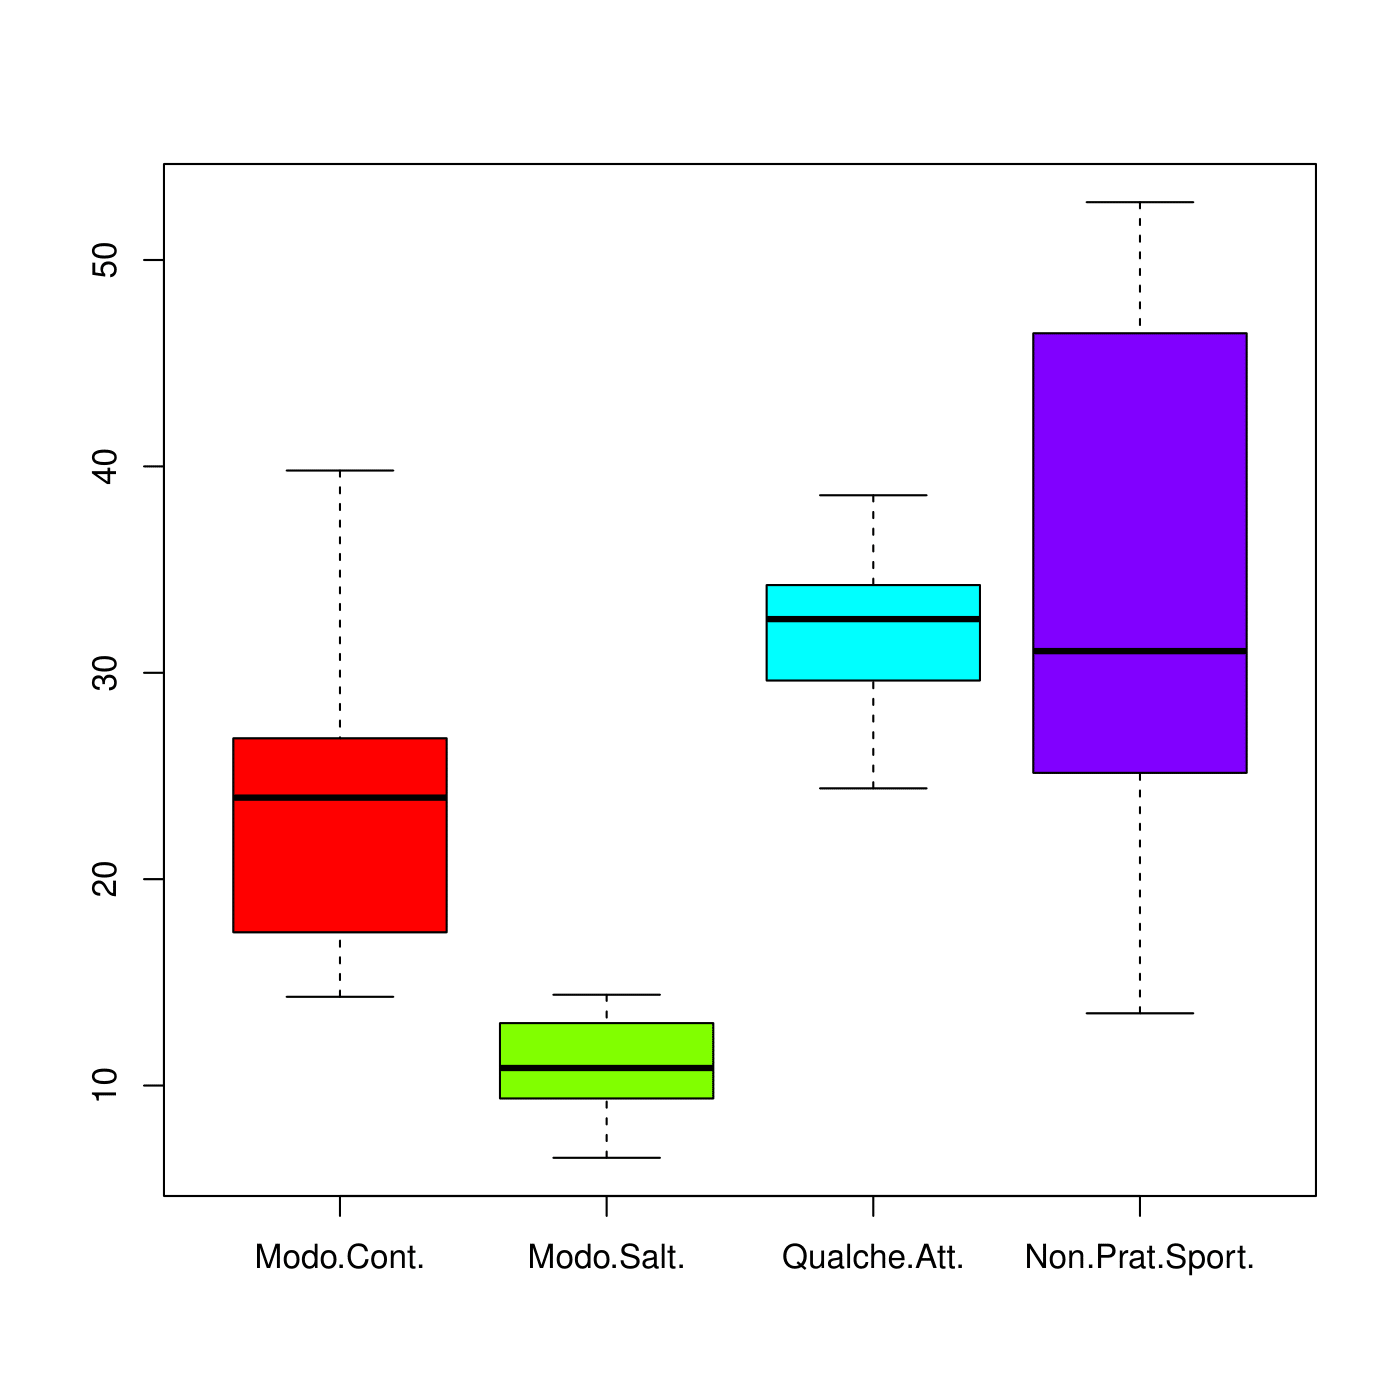
\includegraphics[height=14cm]{ProgettoSAD/capitoli/images/s_desc_univ/quantili_boxplot.png}
    \label{fig:quantili_boxplot}
\end{figure}

Tramite i boxplot ottenuti possiamo fare un'analisi sulla centralità, forma, dispersione e sulla presenza o meno di valori anomali (outlier) della distribuzione di frequenza delle varie caratteristiche. In particolare, si ha che la centralità è espressa dalla mediana. La forma simmetrica o asimmetrica può essere dedotta esaminando le distanze del primo e del terzo quartile dalla linea mediana. I baffi, superiore e inferiore, forniscono informazioni sulla dispersione, sulla forma della distribuzione e anche sulle code della distribuzione. Infatti, la dispersione è deducibile esaminando le distanze del baffo superiore da $Q_3$ e del baffo inferiore da $Q_1$. Inoltre, il baffo inferiore corrisponde al valore più piccolo tra le osservazioni che risulta maggiore o uguale di $Q_1 - 1.5 * (Q_3 - Q_1)$, mentre il baffo superiore corrisponde al valore più grande delle osservazioni che risulta minore o uguale a $Q_3 + 1.5 * (Q_3 - Q_1)$. 

Tra le diverse caratteristiche non sono presenti valori anomali, infatti tutte le caratteristiche rientrano nell'intervallo $Q_1 - 1.5 * (Q_3 - Q_1)$, $Q_3 + 1.5 * (Q_3 - Q_1)$ e i baffi sono posti in corrispondenza del minimo e del massimo.

È presente in tutte le caratteristiche una leggera asimmetria nei dati, poiché la mediana non sembra trovarsi in nessuno dei quattro casi al centro della distribuzione, non essendo dunque utile per avere un valore medio giusto dei dati, ma in tutti i casi il baffo inferiore coincide con il \textit{valore minimo} e il baffo superiore coincide con il \textit{valore massimo}.

Nei casi di svolgimento in Modo Saltuario e Non Praticano Sport la mediana è spostata verso il primo quartile, non risultando utile per avere un valore medio giusto dei dati, mentre nello svolgimento in Modo Continuativo e Qualche Attività la mediana è spostata verso il terzo quartile.

\section{Indici di sintesi: Dispersione dei dati}\label{cap3.2}

Gli indici di posizione non tengono conto della variabilità dei dati; infatti, esistono distribuzioni di frequenza che sono molto diverse tra loro, pur avendo la \textit{stessa media campionaria}. Indici significativi per misurare la variabilità dei dati sono la \textit{varianza campionaria} e la \textit{deviazione standard campionaria}. Tali indici sono detti \textit{indici di dispersione} o \textit{indici di variabilità} poichè misurano la dispersione dei dati \textit{intorno alla media}.

\subsection{Varianza}\label{cap3.2.1}

\noindent \textbf{Definizione:} Assegnato un insieme di dati numerici $x_1, x_2, ..., x_n$, si definisce \textbf{\textit{varianza campionaria}} e si denota con $s^2$ la quantità:

\[s^2 = \frac{1}{n-1} \sum_{i=1}^n (x_i - \bar x)^2 \quad \quad (n = 2, 3, ...) \]

dove $\Bar{x}$ denota la media campionaria dei dati. La varianza identifica il valore della dispersione dei dati intorno al valore medio.

In R la varianza campionaria può essere facilmente calcolata tramite la funzione var().

\vspace{5mm}
\noindent \textbf{Varianza delle caratteristiche del dataset}


\begin{lstlisting}
varianzaCaratteristiche <- function(df) {
  variance <- data.frame(Variance = c(
    var(df$Modo.Cont.),
    +var(df$Modo.Salt.),
    +var(df$Qualche.Att.),
    +var(df$Non.Prat.Sport)))
  row.names(variance) <- names(df)
  variance
}
\end{lstlisting}
\vspace{5mm}

\vspace{5mm}
\begin{tabular}{ c c}
  & Variance\\
 Modo.Cont & 41.671868\\ 
 Modo.Salt & 6.196289\\
 Qualche.Att & 18.043447\\ 
 Non.Prat.Sport & 140.827263\\ 
\end{tabular}
\vspace{5mm}

Dai risultati ottenuti si può notare che la varianza per le frequenze Modo Saltuario e Qualche Attività la varianza è meno elevata, quindi con dati più compatti, mentre per le frequenze Modo Continuativo e Non Praticano Sport la varianza è molto più alta, indicando un maggiore scostamento della media.

\subsection{Deviazione standard}\label{cap3.2.2}

\noindent \textbf{Definizione:} Si definisce \textbf{\textit{deviazione standard campionaria}} e si denota con $s$ la radice quadrata della \textit{varianza campionaria}, ossia:

\[s = \sqrt{\frac{1}{n-1} \sum_{i=1}^n (x_i - \bar x)^2} \quad \quad (n = 2, 3, ...)\]

La deviazione standard è un indice di quanto i numeri si distanzino dalla media aritmetica, cioè quanto i valori di una distribuzione si discostino dalla media stessa. In R la deviazione standard campionaria può essere facilmente calcolata attraverso la funzione \textit{sd()}.

\vspace{5mm}
\noindent \textbf{Deviazione standard delle caratteristiche del dataset}

\vspace{5mm}
\begin{lstlisting}
devStandardCaratteristiche <- function(df) {
  sd <- data.frame(Deviazione_standard = c
  (sd(df$Modo.Cont), sd(df$Modo.Salt.),
   sd(df$Qualche.Att.), sd(df$Non.Prat.Att.)))
  row.names(sd) <- names(df)
  sd
}
\end{lstlisting}
\vspace{5mm}

\vspace{5mm}
\begin{tabular}{ c c}
  & Deviazione Caratteristiche\\
 Modo.Cont & 6.455375\\ 
 Modo.Salt & 2.489235\\
 Qualche.Att & 4.247758\\ 
 Non.Prat.Sport & 11.867066\\ 
\end{tabular}
\vspace{5mm}

\subsection{Coefficiente di variazione}\label{cap3.2.3}

Per confrontare le variazioni esistenti tra diversi campioni di dati è utile introdurre il \textit{coefficiente di variazione}. Esso è un \textit{indice adimensionale} che non dipende dall'unità di misura dei dati. Inoltre, tale indice viene usato anche in insiemi di dati aventi differenti \textit{range di variazione} (il range di variazione è dato dalla differenza tra il massimo e il minimo dei dati.

\noindent \textbf{Definizione:} Assegnato un insieme di dati numerici $x_1, x_2, ..., x_n$, si definisce \textbf{\textit{coefficiente di variazione}} il rapporto tra la \textit{deviazione standard campionaria} e il modulo della \textit{media campionaria}, ossia

\[CV = \frac{s}{|\bar x|}\]

In R non è definita una funzione che calcola il coefficiente di variazione. Tale funzione può essere comunque implementata in R nel seguente modo:

\vspace{5mm}
\begin{lstlisting}
cv <- function(x){
    sd(x)/abs(mean(x))
}
\end{lstlisting}
\vspace{5mm}

\noindent \textbf{Coefficiente di variazione delle caratteristiche del dataset}

\vspace{5mm}
\begin{lstlisting}
coeffVarCaratteristiche <- function(df) {
  cvCoefficient <- data.frame(Variation_Coefficient = c
  (cv(df$Modo.Cont), cv(df$Modo.Salt),
   cv(df$Qualche.Att.), cv(df$Non.Prat.Sport.)))
  row.names(cvCoefficient) <- names(df)
  cvCoefficient
}
\end{lstlisting}
\vspace{5mm}

\vspace{5mm}
\begin{tabular}{ c c}
  & Coefficiente di Variazione\\
 Modo.Cont & 0.2737068\\ 
 Modo.Salt & 0.2274312\\
 Qualche.Att & 0.1334304\\ 
 Non.Prat.Sport & 0.3530814\\ 
\end{tabular}
\vspace{5mm}

Come si evince dai dati ottenuti il coefficiente di variazione più alto si ottiene per la caratteristica Non Praticano Sport, indicando che questi sono i dati che hanno un maggior range di variazione. Inoltre, poichè ogni coefficiente di variazione è inferiore a 1, vuol dire che la media è significativa nei dati.

\section{Forma di una distribuzione di frequenza}\label{cap3.3}

La media e  la mediana sono utili a comprendere la forma delle distribuzioni di frequenza, nel senso che differenze sostanziali tra questi indici indicano uno sbilanciamento eccessivo della distribuzione di frequenza verso destra o verso sinistra. Esistono degli indici statistici che permettono di misurare quando una distribuzione di frequenza presenta simmetria o asimmetria oppure se essa è più o meno piccata.

\subsection{Skewness}\label{cap3.3.1}

La skewness campionaria misura la simmetria di una distribuzione di frequenza.

\noindent \textbf{Definizione:} Assegnato un insieme di dati numerici $x_1, x_2, ..., x_n$, si definisce skewness campionaria il valore:

\[\gamma_1 = \frac{m_3}{m_2^{3/2}}\]

dove $m_3$ denota il momento centrato campionario di ordine 3. In generale, il momento centrato campionario di ordine j è così definito:

\[m_j = 1/n \sum_i=1^n (x_i - \bar x)^j \quad \quad (j = 1, 2, ...)\]

Dalla definizione si ha che:

\begin{itemize}
\item Se $\gamma_1 = 0$ allora la distribuzione di frequenza è simmetrica;
\item Se $\gamma_1 > 0$ allora la distribuzione di frequenza ha la coda di destra più allungata (asimmetria positiva);
\item Se $\gamma_1 < 0$ allora la distribuzione di frequenza ha la coda di sinistra più allungata (asimmetria negativa);
\end{itemize}

In R non esiste una funzione che calcoli la skewness, ma può essere facilmente creata:

\vspace{5mm}
\begin{lstlisting}
skw <- function(x) {
  n <- length(x)
  m2 <- (n - 1) * var(x) / n
  m3 <- (sum((x - mean(x))^3)) / n
  m3 / (m2^1.5)
}
\end{lstlisting}
\vspace{5mm}

Si può ora applicare la funzione alle caratteristiche del dataset, ottenendo:

\vspace{5mm}
\begin{lstlisting}
    skw(df$Modo.Cont.)
    [1] 0.4664549
    skw(df$Modo.Salt.)
    [1] -0.3042624
    skw(df$Qualche.Att.)
    [1] -0.4078287
    skw(df$Non.Prat.Sport.)
    [1] 0.366378
\end{lstlisting}
\vspace{5mm}

Dai risultati ottenuti si ha che le caratteristiche Modo Continuativo e Non Pratica Sport hanno una chiara asimmetria positiva, mentre le caratteristiche Modo Saltuario e Qualche Attività presentano un'asimmetria negativa.

\subsection{Curtosi}\label{cap3.3.2}

La curtosi campionaria permette di misurare la densità dei dati intorno alla media.

\noindent \textbf{Definizione:} Assegnato un insieme di dati numerici $x_1, x_2, ..., x_n$, si definisce curtosi campionaria il valore:

\[\gamma_2 = \beta_2 - 3\]

dove

\[\beta_2 = \frac{m_4}{m_2^2}\]

avendo denotato con $m_4$ il momento centrato campionario di ordine 4. Se risulta:

\begin{itemize}
\item $\beta_2 < 3$, $\gamma_2<0$ allora la distribuzione di frequenza si definisce platicurtica, ossia la distribuzione di frequenza è più piatta di una normale.
\item $\beta_2 > 3$, $\gamma_2 > 0$ allora la distribuzione si definisce leptocurtica, ossia la distribuzione di frequenza è più piccata di una normale;
\item $\beta_2 = 3$, $\gamma_2 = 0$ allora la distribuzione di frequenza si definisce normocurtica, ossia la distribuzione di frequenza è piatta come una normale;
\end{itemize}

Anche in questo caso non esiste una funzione in R che calcoli tale indice, ma può essere così formulata:

\vspace{5mm}
\begin{lstlisting}
curt <- function(x) {
  n <- length(x)
  m2 <- (n - 1) * var(x) / n
  m4 <- (sum((x - mean(x))^4)) / n
  m4 / (m2^2) - 3
}
\end{lstlisting}
\vspace{5mm}

Si può ora applicare la funzione alle caratteristiche del dataset, ottenendo:

\vspace{5mm}
\begin{lstlisting}
    curt(df$Modo.Cont.)
    [1] 0.2121162
    curt(df$Modo.Salt.)
    [1] -1.002682
    curt(df$Qualche.Att.)
    [1] -0.8136908
    curt(df$Non.Prat.Sport.)
    [1] -1.05531
\end{lstlisting}
\vspace{5mm}

La curtosi risulta negativa per le caratteristiche Modo Saltuario, Qualche Attività e Non Pratica Sport, ovvero la distribuzione di frequenza è più piatta di una normale, mentre è positiva per Modo Continuativo, ovvero la distribuzione di frequenza è più piccata di una normale.

\vspace{5mm}
\noindent \textbf{Istogrammi}

Per poter osservare in maniera grafica ciò che si è ottenuto dagli indici di skewness e curtosi campionaria si possono osservare i seguenti istogrammi relativi alle caratteristiche.

\vspace{5mm}
\begin{lstlisting}
istogrammi <- function(df) {
  hist(df$Modo.Cont., freq = TRUE, main = " Istogramma
    Modo Continuativo ", xlab = " Modo Continuativo ", ylab = "
    Percentuale ")
  hist(df$Modo.Salt., freq = TRUE, main = " Istogramma
    Modo Saltuario ", xlab = " Modo Saltuario ", ylab = "
    Percentuale ")
  hist(df$Qualche.Att., freq = TRUE, main = " Istogramma
    Qualche Attivit " , xlab = " Qualche Attività ", ylab = "
    Percentuale ")
  hist(df$Non.Prat.Sport, freq = TRUE, main = " Istogramma
    Non Pratica Sport ", xlab = " Non Pratica Sport ", ylab = "
    Percentuale ")
}
\end{lstlisting}
\vspace{5mm}

Dal codice precedente si ottengono i seguenti istogrammi:

\begin{figure}[!htbp]
    \centering
        \subfloat{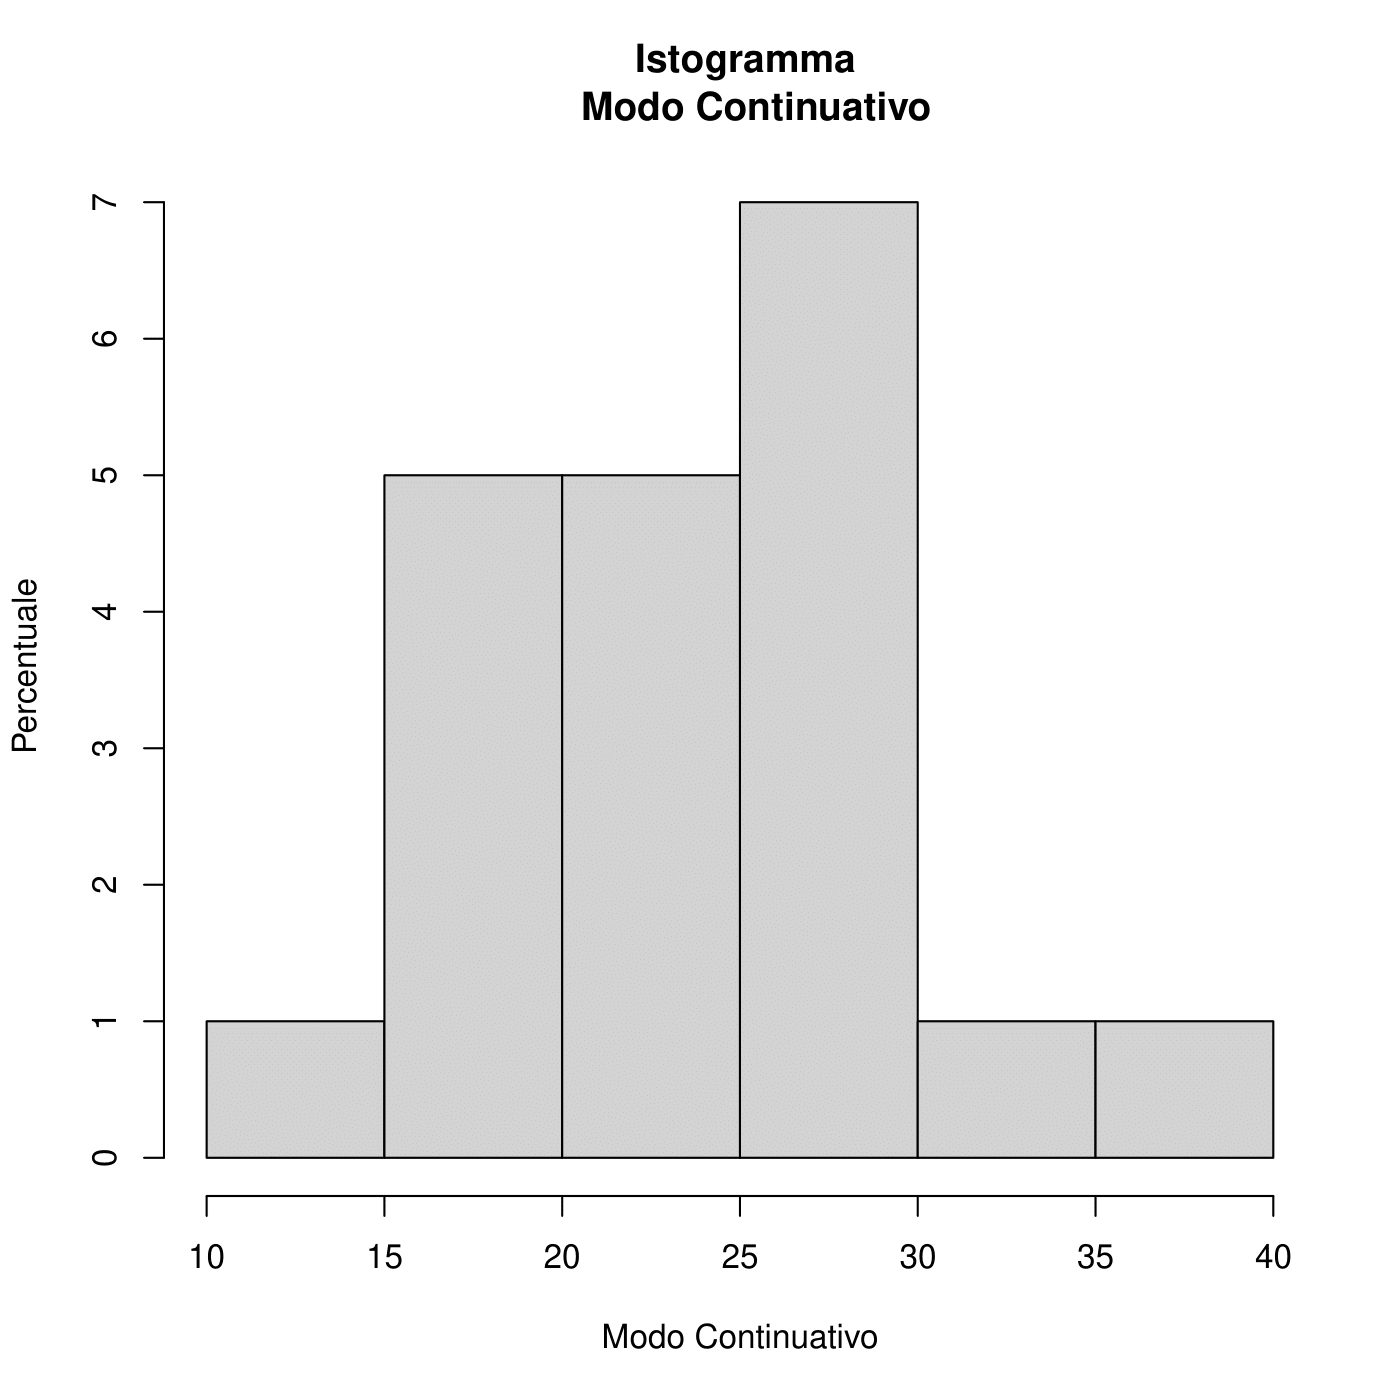
\includegraphics[height=8cm]{ProgettoSAD/capitoli/images/s_desc_univ/hist_modocont.png}}
        \qquad
        \subfloat{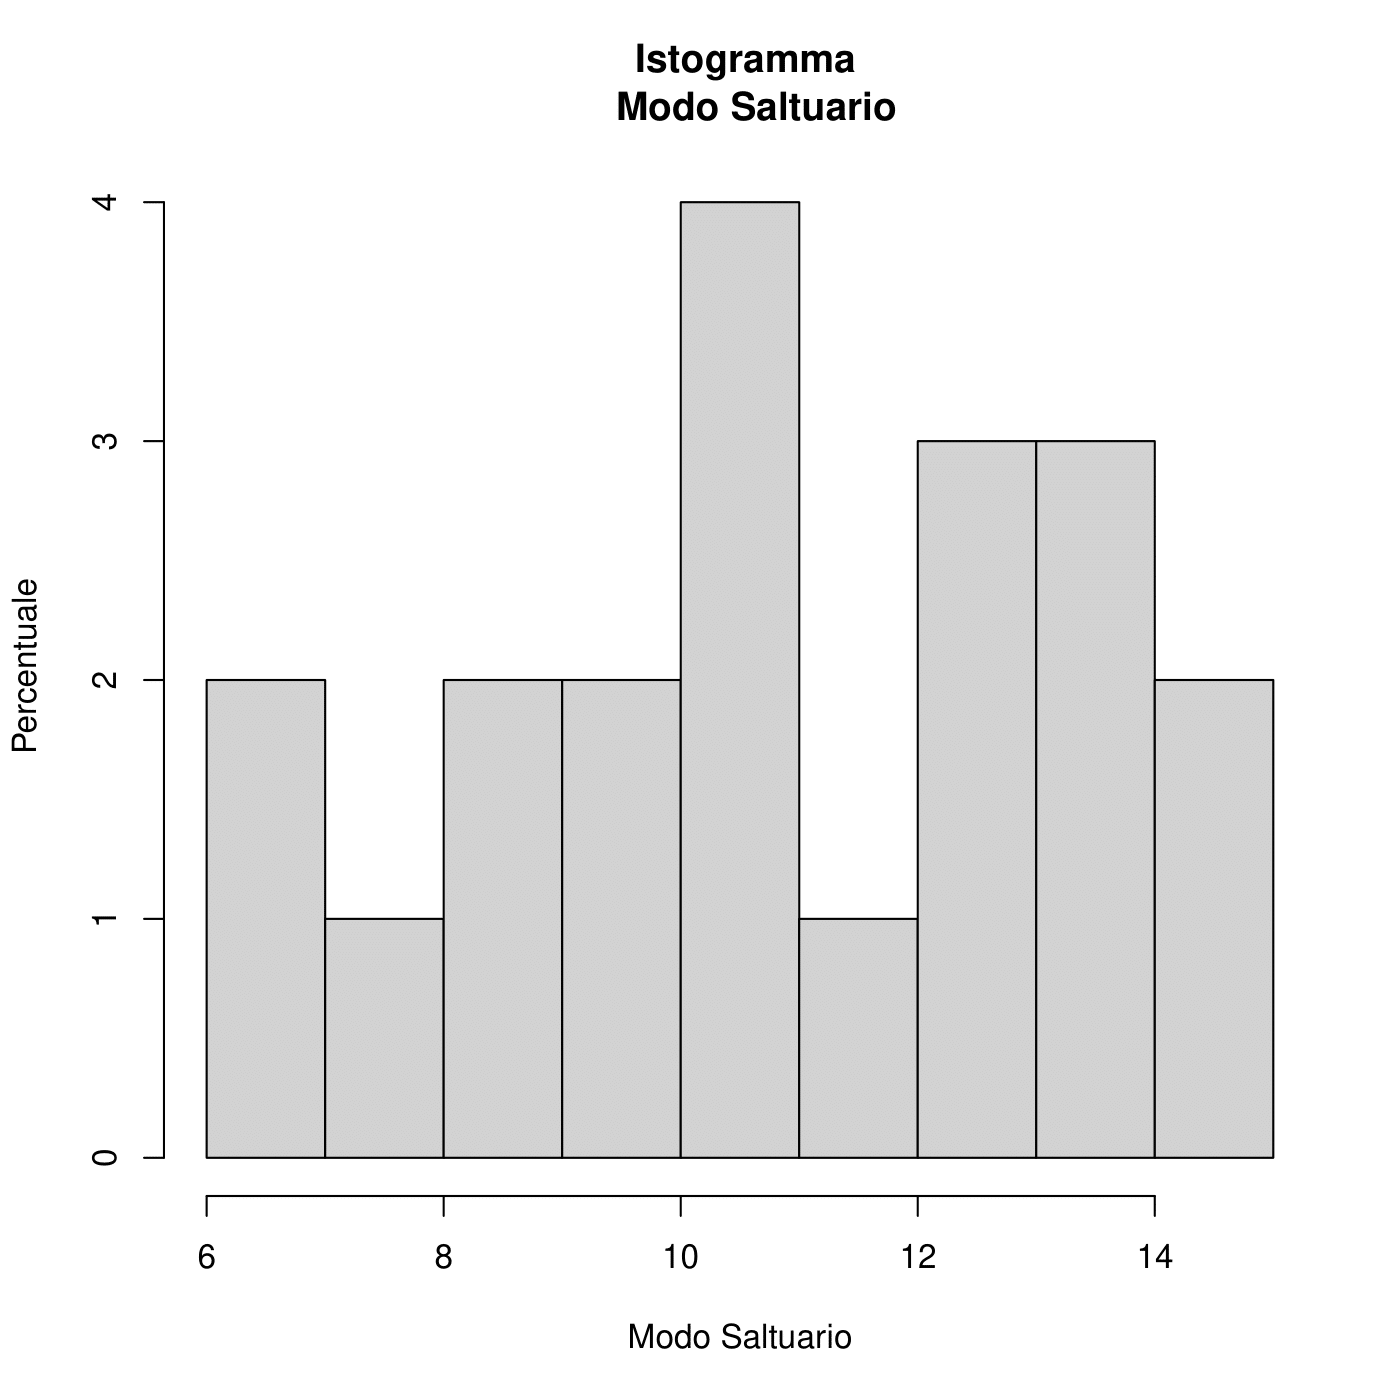
\includegraphics[height=8cm]{ProgettoSAD/capitoli/images/s_desc_univ/hist_modosalt.png}}
        \qquad
\end{figure}
\begin{figure}[!htbp]
    \centering
        \subfloat{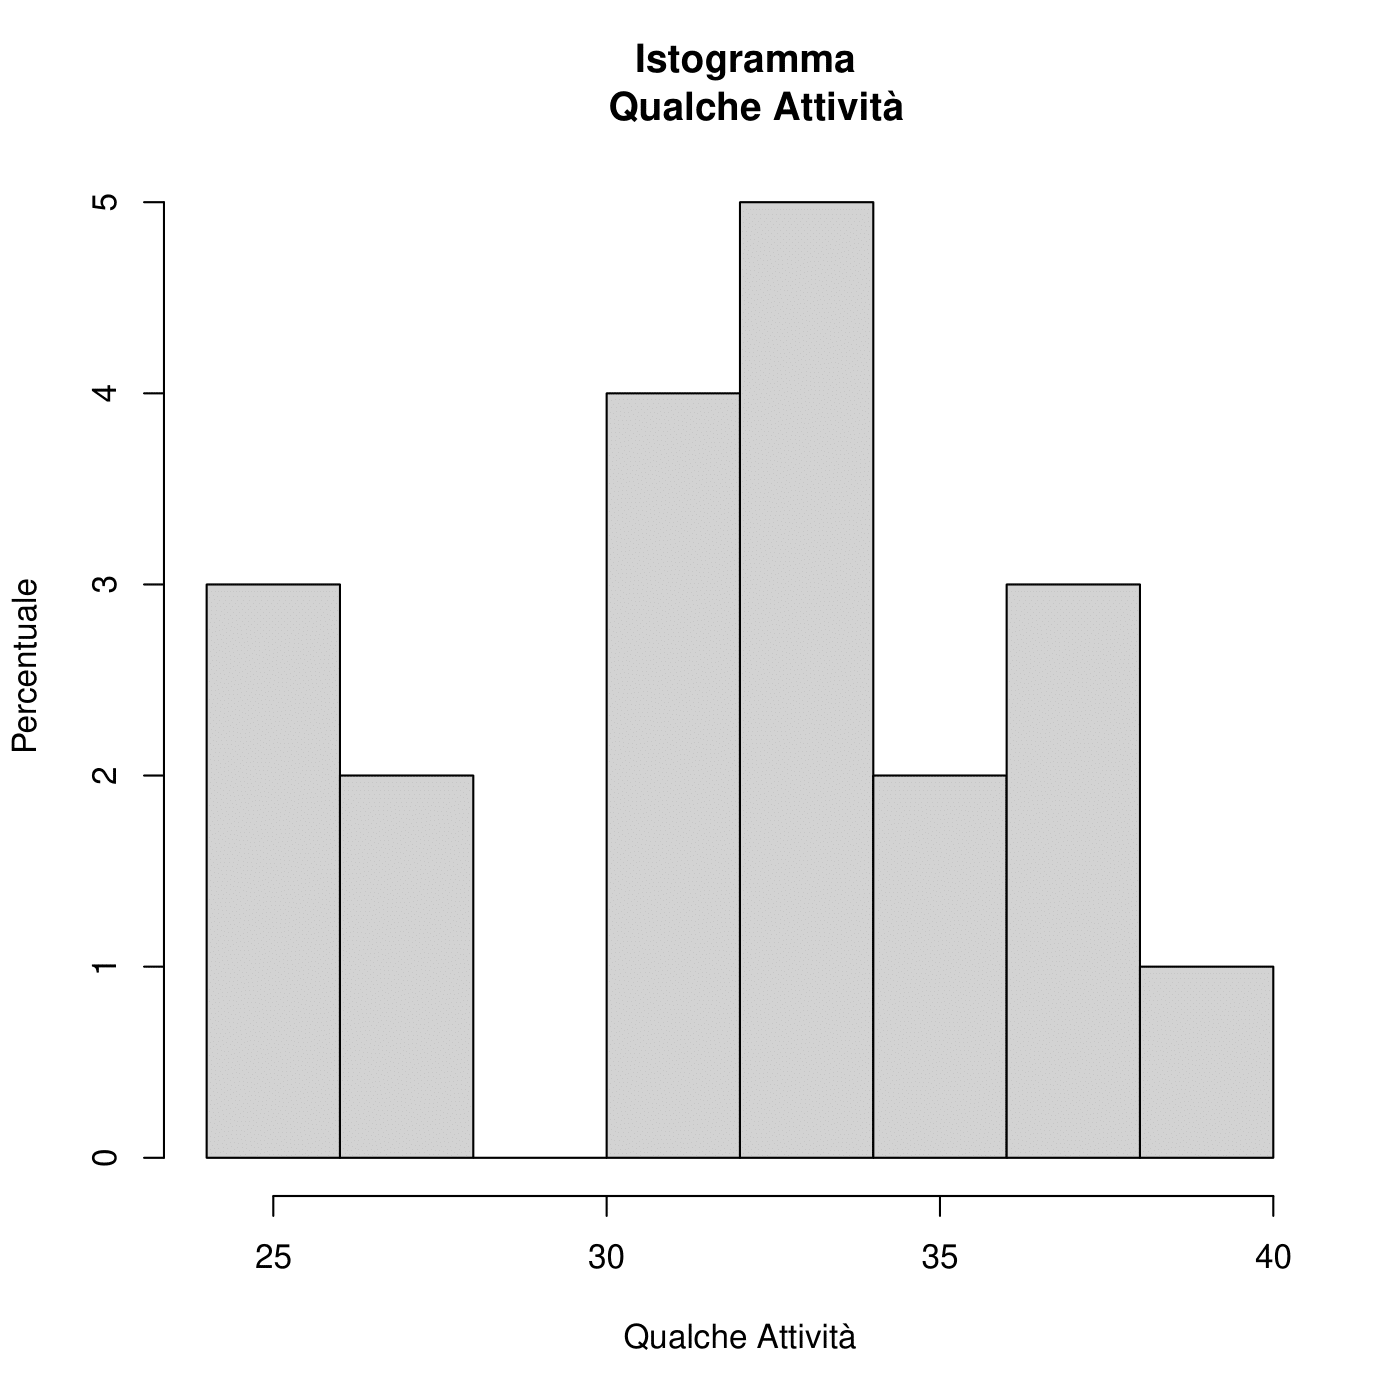
\includegraphics[height=8cm]{ProgettoSAD/capitoli/images/s_desc_univ/hist_qualcheatt.png}}
        \qquad
        \subfloat{\includegraphics[height=8cm]{ProgettoSAD/capitoli/images/s_desc_univ/hist_nonpratsport.png}}
        \qquad
\end{figure}

%################################################

\newpage
\phantomsection
\definecolor{dkgreen}{rgb}{0,0.6,0}
\definecolor{gray}{rgb}{0.5,0.5,0.5}
\definecolor{mauve}{rgb}{0.58,0,0.82}


\lstset{frame=tb,
language=R,
aboveskip=3mm,
belowskip=3mm,
showstringspaces=false,
columns=flexible,
numbers=none,
inputencoding=utf8/latin1,
keywordstyle=\color{blue},
numberstyle=\tiny\color{gray},
commentstyle=\color{dkgreen},
stringstyle=\color{mauve},
breaklines=true,
breakatwhitespace=true,
tabsize=3
}

\chapter{Statistica Descrittiva Bivariata}\label{cap4}

In questo capitolo si sviluppa la statistica descrittiva bivariata, ossia il ramo della statistica che si occupa dei metodi grafici e statistici atti a descrivere le relazioni tra \textit{due} variabili quantitative.

Dopo aver scelto la variabile da porre sulle ascisse (variabile indipendente) \textit{X} e la variabile da porre sulle ordinate (variabile dipendente) \textit{Y}, si disegnano dei punti in corrispondenza delle coppie ($x_i, y_i$). Ciò che si ottiene disegnando tali punti mediante \textit{diagrammi di dispersione} (scatterplot) è una nuvola di punti che evidenzia, se esiste, una qualche \textit{forma di regolarità}, o meglio una qualche \textit{forma di relazione} tra le variabili.

In particolare si analizzeranno le relazioni tra i dati presenti attraverso indici di covarianza campionaria, coefficiente di correlazione campionario e vari grafici. Successivamente si andrà ad osservare la regressione lineare semplice, multipla e non lineare.

\section{Covarianza e correlazione campionaria}\label{cap4.1}

Spesso nelle indagini statistiche si osservano più variabili quantitative per uno stesso gruppo di individui e, in tal caso, è necessario vedere se esiste una correlazione tra le variabili.

\subsection{Covarianza campionaria}\label{cap4.1.1}

Per ottenere una misura quantitativa della correlazione tra le variabili si considera la \textit{covarianza campionaria}.

\noindent \textbf{Definizione:} Assegnato un campione bivariato ($x_1, y_1$), ($x_2, y_2$), ..., ($x_n, y_n$), di una variabile quantitativa bidimensionale (X, Y), siano $\bar x$ e $\bar y$ rispettivamente le medie campionarie di $x_1, x_2, ..., x_n$ e di $y_1, y_2, ..., y_n$. La \textbf{\textit{covarianza campionaria}} tra le due variabili X e Y è così definita:

\[C_{xy} = \frac{1}{n-1} \sum_{i=1}^n (x_i - \bar x)(y_i - \bar y) \quad \quad (n = 2, 3, ...)\]

In R la covarianza campionaria può essere facilmente calcolata con la funzione \textit{cov}

\vspace{5mm}
\noindent \textbf{Covarianza Campionaria delle caratteristiche del dataset}

\vspace{5mm}
\begin{lstlisting}
round(cov(df),digits = 2)
\end{lstlisting}
\vspace{5mm}

\vspace{5mm}
\begin{tabular}{c c c c c}
 & Modo.Cont. & Modo.Salt. & Qualche.Att & Non.Prat.Sport\\
 Modo.Cont. & 41.67 & 13.49 & 16.49 & -71.80\\
 Modo.Salt. & 13.49 & 6.20 & 7.21 & -26.92\\
 Qualche.Att. & 16.49 & 7.21 & 18.04 & -41.82\\
 Non.Prat.Sport & -71.80 & -26.92 & -41.82 & 140.83\\
\end{tabular}
\vspace{5mm}

Osservando i valori della covarianza si può notare come nella maggior parte dei casi i valori sono positivi ($C_{xy} > 0$), ovvero le variabili associate a tali valori sono correlate positivamente. Valori troppo bassi, però, denotano una scarsa correlazione. Nella colonna della caratteristica Non Praticano Sport, alcuni dei valori sono però negativi, simbolo di una correlazione negativa. Possiamo notare come sulla diagonale sono presenti i valori della varianza osservati in precedenza.

\subsection{Correlazione campionaria}\label{cap4.1.2}

Per ottenere una misura quantitativa della correlazione tra le variabili si può anche considerare il coefficiente di correlazione campionario 

\noindent \textbf{Definizione:} Assegnato un valore bivariato ($x_1, y_1$), ($x_2, y_2$), ..., ($x_n, y_n$) di una variabile quantitativa bidimensionale (X,Y) siano $\bar x$ e $s_x$ la media campionaria e la deviazione standard campionaria di $x_1, x_2, ..., x_n$ e siano $\bar y$ e $s_y$  la media campionaria e la deviazione standard campionaria di $y_1, y_2, ..., y_n$. Il \textbf{\textit{coefficiente di correlazione campionario}} tra le due variabili X e Y è così definito:

\[r_{xy} = \frac{C_{xy}}{s_{x} s_{y}}\]

In R il coefficiente di correlazione campionario può essere facilmente calcolato con la funzione \textit{cor()}.

\noindent \textbf{Coefficiente di correlazione delle caratteristiche del dataset}

\vspace{5mm}
\begin{lstlisting}
    round(cor(df), digits = 2)
\end{lstlisting}
\vspace{5mm}

\vspace{5mm}
\begin{tabular}{c c c c c}
 & Modo.Cont. & Modo.Salt. & Qualche.Att & Non.Prat.Sport\\
 Modo.Cont. & 1.00 & 0.84 & 0.60 & -0.94\\
 Modo.Salt. & 0.84 & 1.00 & 0.68 & -0.91\\
 Qualche.Att. & 0.60 & 0.68 & 1.00 & -0.83\\
 Non.Prat.Sport & -0.94 & -0.91 & -0.83 & 1.00\\
\end{tabular}
\vspace{5mm}

In modo analogo alla covarianza campionaria, il coefficiente di correlazione campionario indica la relazione tra i dati del campione, ottenendo anche in questo caso non soltanto correlazioni positive ma anche negative. Si nota che sulla diagonale troviamo il valore 1 poiché una caratteristica è correlata al massimo con se stessa con tutti i punti allineati su una \textbf{linea retta ascendente}, mentre gli altri valori indicano un rapporto di relazione non influenzato dalle unità di misura dei dati. Il coefficiente di correlazione campionario, inoltre, indica che se 0 < $r_{xy}$ < 1 allora i punti $x_i, y_i$ sono posizionati in una nuvola attorno a una linea \textbf{retta interpolante ascendente}, mentre se -1 < $r_{xy}$ < 0 allora i punti $x_i, y_i$ sono posizionati in una nuvola attorno a una linea \textbf{retta interpolante discendente}

\section{Regressione lineare semplice}\label{cap4.2}

Il \textit{modello di regressione lineare} semplice è esprimibile attraverso l'equazione di una retta che riesce a interpolare la nuovola di punti dello scatterplot meglio di tutte le altre possibili rette. Consideriamo l'equazione della retta: 

\[Y = \alpha + \beta X\]

\noindent dove

\begin{itemize}
    \item $\alpha$ è l'intercetta: corrisponde all'ordinata del punto di intersezione della retta interpolante (di regressione) con l'asse delle ordinate.
    \item $\beta$ è il coefficiente angolare: esprime l'inclinazione della retta.
\end{itemize}

In questo paragrafo si andrà ad analizzare la regressione lineare semplice per un sottoinsieme di dati, poiché analizzare tutto il dataset risulterebbe oneroso. Lo studio della regressione lineare semplice verrà effettuato sulla base di due caratteristiche del dataset, ponendo:

\begin{itemize}
    \item \textbf{Variabile indipendente: Modo Continuativo}
    \item \textbf{Variabile dipendente: Qualche Attività}
\end{itemize}

\noindent \textbf{Scatterplot delle due variabili considerate}

Con il seguente codice si va a disegnare lo scatterplot (diagramma di dispersione) delle due variabili.

\begin{figure}[!htbp]
    \centering
    \includegraphics[height=16cm]{ProgettoSAD/capitoli/images/s_desc_biv/scatterplot_variabili.pdf}
\end{figure}

Dal grafico ottenuto si nota che la nuvola di dati sembra posizionarsi intorno a una retta ascendente, inducendo a pensare che esista una correlazione lineare positiva tra entrambe le variabili. Nel grafico sono anche stati evidenziati i valori della media (linea retta) e della mediana (linea tratteggiata) per entrambe le caratteristiche che appaiono rosse per la caratteristica Modo Continuativo e arancioni per la caratteristica Qualche Attività.

\noindent \textbf{Calcolo della retta di regressione}

Al fine di poter disegnare la retta di regressione ($Y = \alpha + \beta X$) che interpola i punti nel grafico si vanno a calcolare i parametri $\alpha$ e $\beta$ di tale retta con il seguente codice, impiegando la funzione \textit{lm(y $\sim$ x)(linear model)}.

\vspace{5mm}
\begin{lstlisting}
  lm_reg <- lm(df$Qualche.Att. ~ df$Modo.Cont.)
  lm_reg

    Call:
    lm(formula = df$Qualche.Att. ~ df$Modo.Cont.)
    
    Coefficients:
      (Intercept)  df$Modo.Cont.  
          22.5033         0.3957    
\end{lstlisting}
\vspace{5mm}
 
Disegnando, attraverso la funzione \textit{abline(lm\_reg)} la retta

\[Y = 22.5033 + 0.3957X\]

sul grafico precedente

\vspace{5mm}
\begin{lstlisting}
  plot(df$Modo.Cont., df$Qualche.Att., main = " Retta di regressione relativa a
  Modo Continuativo e Qualche Attività ",
       xlab = " Modo Continuativo ",
       ylab = " Qualche Attività ", col = " blue ")
  abline(rettaRegressione(df), col = " red ")
\end{lstlisting}
\vspace{5mm}

si ottiene:

\begin{figure}[!htbp]
    \centering
    \includegraphics[height=16cm]{ProgettoSAD/capitoli/images/s_desc_biv/retta_regressione.pdf}
\end{figure}

\subsection{Residui}\label{cap4.2.1}

Una volta calcolati i valori dei coefficienti $\alpha$ e $\beta$ e disegnata la retta di regressione che interpola la nuvola dei punti nel corrispondente scatterplot, è possibile osservare quanto questa retta si adatta ai punti che individuano le osservazioni. 

In generale, esisteranno degli scostamenti (\textbf{residui}) tra le ordinate dei punti $y_i$ (\textit{valori osservati)} e i corrispondenti \textit{valori stimati}

\[\hat{y_i} = \alpha + \beta x_i \quad \quad (i = 1, 2, ..., n)\]

ottenuti mediante la retta di regressione. I punti ($x_1, \hat{y_1}$), ($x_2, \hat{y_2}$), ..., ($x_n, \hat{y_n}$) sono posizionati sulla retta di regressione. 

I residui,

\[E_i = y_i - \hat{y_i} = y_i - (\alpha + \beta x_i) \quad \quad (i = 1, 2, ..., n)\]

dunque, mostrano di quanto si discostano i valori osservati dai valori stimati con la retta di regressione. Inoltre, la media campionaria dei residui $E$ è nulla, ossia in media gli scostamenti positivi e negativi si compensano

\noindent \textbf{Valori stimati}

In R per calcolare il vettore dei valori stimati ($\hat{y_1}, \hat{y_2}, ..., \hat{y_n}$) si utilizza la funzione \textit{fitted()}, ottenendo:

\vspace{5mm}
\begin{lstlisting}
    stime <- fitted(lm(df$Modo.Cont. ~ df$Qualche.Att.))
    stime


       1        2        3        4        5 
32.79052 35.36232 31.64310 33.58184 38.25064 
       6        7        8       9       10 
33.50271 32.07833 33.58184 32.98835 31.8805 
      11       12       13       14       15
32.59269 32.71139 31.80137 28.59652 28.16129
      16      17       18       19       20 
29.58567 28.83391 28.75478 28.67565 31.32658 
\end{lstlisting}
\vspace{5mm}

Ad esempio, il primo valore stimato (32.79) è il risultato di $\hat{y_1} = \alpha + \beta x_1 = 22.5033 + 0.3957 * 26$, dove 26 è il dato percentuale del primo elemento del dataset nella \textit{caratteristica indipendente} (Modo Continuativo).

\vspace{5mm}
\noindent \textbf{Residui}
\vspace{5mm}

In R per calcolare il vettore dei residui ($E_1, E_2, ..., E_n$) si utilizza la funzione \textit{resid()}, ottenendo:

\vspace{5mm}
\begin{lstlisting}
    residui <- resid(lm(df$Qualche.Att. ~ df$Modo.Cont.))
    residui


         1          2          3          4          5
-1.2905206 -1.4623152  6.9568954  2.8181580 -6.0506384
         6          7          8          9         10
 0.8972901  5.3216687  0.6181580  1.0116490  1.1194990
        11         12         13         14         15
 0.6073097 -0.9113885 -0.8013688  1.6034829 -1.8612903 
        16         17         18         19         20 
-5.1856689 -3.5339135 -0.8547814 -4.0756492  5.0734240
\end{lstlisting}
\vspace{5mm}

Ad esempio, il primo valore stimato (-1.29) è il risultato di $y_1 - \hat{y_1} = 31.5 - 32.79 $, dove 31.5 è il dato percentuale del primo elemento del dataset nella \textit{caratteristica dipendente} (Qualche Attività), mentre 32.79 è il valore stimato precedentemente.

\vspace{5mm}
\noindent \textbf{Disegno dei Residui}

Il seguente codice disegna i residui, ovvero dei segmenti che congiungono i \textit{valori stimati} (punti sulla retta) e i \textit{valori osservati}.

\vspace{5mm}
\begin{lstlisting}
  plot(df$Modo.Cont., df$Qualche.Att., main = " Retta di regressione relativa
  a Modo Continuativo e Qualche Attività ",
       xlab = " Modo Continuativo ",
       ylab = " Qualche Attività ", col = " blue ")
  abline(rettaRegressione(df), col = " red ")
  segments(df$Modo.Cont., fitted(lm(df$Qualche.Att. ~ df$Modo.Cont.)), 
           df$Modo.Cont., df$Qualche.Att., col = "green ")
\end{lstlisting}
\vspace{5mm}

\vspace{5mm}
\begin{figure}[!htbp]
    \centering
    \includegraphics[height=16cm]{ProgettoSAD/capitoli/images/s_desc_biv/disegno_residui.pdf}
\end{figure}
\vspace{5mm}

Attraverso la funzione \textit{segments()} è stato possibile disegnare dei segmenti in modo tale da poter osservare gli scostamenti tra i valori stimati e i valori osservati.

\vspace{5mm}
\noindent \textbf{Diagramma dei residui}

Un esame più accurato del modo con cui la retta di regressione interpola i dati e di come i residui si dispongano intorno alla retta interpolante influenzandone la posizione può essere ottenuto attraverso il \textit{diagramma dei residui}, che è un grafico in cui i \textit{valori dei residui} sono posti sull'asse delle ordinate e quelli della \textit{variabile indipendente} sull'asse delle ascisse. Di seguito il codice per costruire il diagramma dei residui con il relativo grafico.

\vspace{5mm}
\begin{lstlisting}
  plot(df$Qualche.Att.,
       residuiValori(df),
       main = " Diagramma dei residui ", xlab = "Modo Continuativo",
       ylab = " Qualche Attività ", pch = 9, col = " blue ")
  abline(h = 0, col =)
\end{lstlisting}
\vspace{5mm}

\vspace{5mm}
\begin{figure}[!htbp]
    \centering
    \includegraphics[height=16cm]{ProgettoSAD/capitoli/images/s_desc_biv/diagramma_residui.pdf}
\end{figure}
\vspace{5mm}

Nel grafico sovrastante si nota come sono disposti i residui rispetto alla variabile indipendente. La retta orizzontale è posizionata nello zero e corrisponde alla media campionaria dei residui, che è nulla. Si nota, inoltre, che i punti sono disposti in maniera abbastanza vicini alla retta, tranne che per alcuni valori che si discostano maggiormente.

Il diagramma dei residui aiuta a comprendere quale è l'adattamento della retta di regressione rispetto ai dati, notando che la posizione di tale retta è fortemente influenzata dalla presenza di eventuali valori anomali. Infatti, tale analisi aiuta a individuare i punti anomali dovuti a errori di stima. Si nota anche che eliminando i valori anomali, la varianza campionaria dei residui diminuisce.

\vspace{5mm}
\noindent \textbf{Residui standardizzati}
\vspace{5mm}

I residui standardizzati

\[E_i^{(s)} = \frac{E_i - \bar{E}}{s_E} = \frac{E_i}{s_E}\]

Risultano essere caratterizzati da media campionaria nulla e varianza unitaria. Di seguito, il codice per costruire il diagramma dei residui standardizzati con il relativo grafico:

\vspace{5mm}
\begin{lstlisting}
  standard_residue <- residuiValori(df) / sd(residuiValori(df))
  plot(stimeValori(df), standard_residue, main = " Residui standard rispetto ai valori stimati "
    , xlab = " Valori stimati ", ylab = " Residui standard ", pch = 4, col = " blue ")
  abline(h = 0, col = " red ", lty = 2)
\end{lstlisting}
\vspace{5mm}

\vspace{5mm}
\begin{figure}[!htbp]
    \centering
    \includegraphics[height=16cm]{ProgettoSAD/capitoli/images/s_desc_biv/residui_standardizzati.pdf}
\end{figure}

Nel grafico sovrastante si nota come sono disposti i residui standardizzati rispetto ai valori stimati con la retta di regressione. La retta orizzontale è posizionata nello zero e corrisponde alla media campionaria dei residui standardizzati. Anche in questo caso i punti sono disposti in maniera abbastanza vicini alla retta, tranne per qualche che si discosta maggiormente.

\subsection{Coefficiente di determinazione}\label{cap4.2.2}

Poichè si è interessati a vedere quanto la retta si adatti ai dati, l'accento può essere posto sul quadrato del coefficiente di correlazione e su quanto esso si avvicini a uno.

\noindent \textbf{Definizione:} Se si denota con ($y_1, y_2, ..., y_n$) il vettore dei dati della variabile dipendente, con $\Bar{y}$ la sua media campionaria e con ($\hat{y_1}, \hat{y_2}, ..., \hat{y_n}$) i valori stimati attraverso la retta di regressione, il \textbf{coefficiente di determinazione} (r-square) è così definito:

\[D^2 = \frac{\frac{1}{n-1} \sum_{i=1}^n (\hat{y_i} - \Bar{y})^2}{\frac{1}{n-1} \sum_{i=1}^n (y_i - \Bar{y})^2} = \frac{\sum_{i=1}^n (\hat{y_i} - \Bar{y})^2}{\sum_{i=1}^n (y_i - \Bar{y})^2}\] 

Si noti che il coefficiente di determinazione è il rapporto tra la varianza dei valori stimati tramite la retta di regressione e la varianza dei valori osservati. Nel caso di regressione lineare semplice, il coefficiente di determinazione coincide con il quadrato del coefficiente di correlazione, ossia

\[D^2 = r_xy^2\]

In R si può calcolare il coefficiente di determinazione in due modi:

\vspace{5mm}
\begin{lstlisting}
(cor(df$Modo.Cont., df$Qualche.Att.))^2
[1] 0.3615508
summary (rettaRegressione(df))$r.square
[1] 0.3615508
\end{lstlisting}
\vspace{5mm}

Ottenendo un coefficiente di determinazione pari a 0.36 si potrebbe pensare che la retta di regressione non approssimi in maniera ottima i dati.

\section{Regressione lineare multipla}\label{cap4.3}

In molte applicazioni dell'analisi di regressione sono coinvolte situazioni con più di una singola variabile indipendente. Il modello di regressione lineare multipla viene utilizzato per spiegare la relazione tra una variabile quantitativa \textit{Y}, detta variabile \textit{dipendente}, e le variabili quantitative \textit{indipendenti} $X_1, X_2, ..., X_p$.

Il modello di \textbf{\textit{regressione lineare multipla}} con \textit{p} variabili indipendenti è esprimibile attraverso l'equazione:

\[Y = \alpha + \beta_1 X_1 + \beta_2 X_2 + ... + \beta_p X_p\]

dove 

\begin{itemize}
    \item $\alpha$ è l'intercetta, ovvero il valore di \textit{Y} quando $X_1 = X_2 = ... = X_p = 0$.
    \item $\beta_1, \beta_2, ..., \beta_p$ sono i regressori, dove $\beta_p$ rappresenta l'inclinazione di \textit{Y} rispetto alla variabile $X_p$ tenendo costanti le variabili $X_1, X_2, ..., X_{p-1}$.
\end{itemize}

Per lo studio della regressione lineare multipla si considera la caratteristica \textbf{Qualche Attività} come \textbf{variabile dipendente}, mentre le restanti variabili vengono considerate indipendenti.

\noindent \textbf{Scatterplot delle variabili}

\vspace{5mm}
\begin{lstlisting}
pairs(df, main = "Scatterplot per le coppie di variabili", col = "blue")
\end{lstlisting}
\vspace{5mm}

\vspace{5mm}
\begin{figure}[!htbp]
    \centering
    \includegraphics[height=16cm]{ProgettoSAD/capitoli/images/s_desc_biv/scatterplot_coppievariabili.pdf}
\end{figure}
\vspace{5mm}

La funzione \textit{pairs()} è in grado di visualizzare in un'unica finestra grafica una pluralità di scatterplot ottenuti mettendo in relazione tutte le coppie di variabili quantitative definite all'interno di un dataframe.

\noindent \textbf{Calcolo della retta di regressione}

Con il seguente codice si vanno a calcolare i valori dell'intercetta e dei regressori della retta:

\vspace{5mm}
\begin{lstlisting}
  lm_multiple <- lm(df$Qualche.Att. ~
                      df$Modo.Cont +
                        df$Modo.Salt. +
                        df$Non.Prat.Sport.)
  lm_multiple


Call:
lm(formula = df$Qualche.Att. ~ df$Modo.Cont + df$Modo.Salt. + 
    df$Non.Prat.Sport.)

Coefficients:
       (Intercept)        df$Modo.Cont       df$Modo.Salt.  df$Non.Prat.Sport.  
           99.6572             -1.0016             -0.9817             -0.9954  
\end{lstlisting}
\vspace{5mm}

In questo modo, si ottiene che l'intercetta è $\alpha = 99.65$, mentre i regressori sono $\beta_1 = -1.0016, \beta_2 = -0.9817, \beta_3 = -0.9954$.
Si può ora costruire la retta, ottenendo:

\[Y = 99.65 - 1.0016x_1 - 0.981x_2 - 0.995x_3\]

\subsection{Residui}\label{cap4.3.1}

Una volta calcolati i valori dei coefficienti $\alpha$, $\beta_1$, $\beta_2$, ..., $\beta_p$ è possibile osservare gli scostamenti (residui) tra le ordinate dei punti $y_i$ (valori osservati) e i corrispondenti valori stimati

\[\hat{y_i} = \alpha + \beta_1 x_{i, 1} + \beta_2 x_{i, 2} + ... + \beta_p x_{i, p} \quad (i = 1, 2, ..., n)\]

ottenuti mediante la regressione lineare multipla. I residui per la regressione multipla

\[E_i = y_i - \hat{y_i} = y_i - (\alpha + \beta_1 x_{i, 1} + \beta_2 x_{i, 2} + ... + \beta_p x_{i, p}) \quad (i = 1, 2, ..., n) \]

mostrano di quanto si discostano i valori osservati dai valori stimati con la retta di regressione. Anche in questo caso, la media campionaria dei residui $\Bar{E}$ è nulla, ossia in media gli scostamenti positivi e negativi si compensano.


\vspace{5mm}
\begin{lstlisting}
  residmulti <- resid(lm_multiple)
  residmulti

           1            2            3            4            5            6 
-0.078197132  0.048600345  0.023909012  0.045688728 -0.018641018  0.016097106 
           7            8            9           10           11           12 
 0.021131470  0.062707286 -0.167089936  0.034344833 -0.053011781  0.054154941 
          13           14           15           16           17           18 
 0.008837465  0.003505733 -0.097860973  0.059077439 -0.022290999  0.115289289 
          19           20 
-0.013064227 -0.043187582  
  
\end{lstlisting}
\vspace{5mm}

\noindent \textbf{Valori stimati}

\vspace{5mm}
\begin{lstlisting}
  stimemulti <- fitted(lm_multiple)
  stimemulti

       1        2        3        4        5        6        7        8 
31.57820 33.85140 38.57609 36.35431 32.21864 34.38390 37.37887 34.13729 
       9       10       11       12       13       14       15       16 
34.16709 32.96566 33.25301 31.74585 30.99116 30.19649 26.39786 24.34092 
      17       18       19       20 
25.32229 27.78471 24.61306 36.44319  
  
\end{lstlisting}
\vspace{5mm}

\noindent \textbf{Residui standardizzati}

Anche nel caso multivariato è interessante calcolare i residui standardizzati. Sono caratterizzati dalla media campionaria nulla e varianza unitaria. Di seguito il codice per costruire il diagramma dei residui standardizzati con il relativo grafico: 

\vspace{5mm}
\begin{lstlisting}
  standard_multi_resid <- residmulti / sd(residmulti)
  plot(stimemulti, standard_multi_resid
    , main =
         " Residui standard rispetto ai valori stimati "
    , xlab = " Valori stimati "
    , ylab = " Residui standard ", pch = 4, col = "blue")
  abline(h = 0, col = " red ", lty = 2)
\end{lstlisting}
\vspace{5mm}

\vspace{5mm}
\begin{figure}[!htbp]
    \centering
    \includegraphics[height=16cm]{ProgettoSAD/capitoli/images/s_desc_biv/residui_standard_multipli.pdf}
\end{figure}
\vspace{5mm}

In questo caso i punti sono disposti quasi casualmente attorno alla retta e non si evidenzia nessuna tendenza particolare nella distribuzione dei punti.

\subsection{Coefficiente di determinazione}\label{cap4.3.2}

Il coefficiente di determinazione di un modello di regressione lineare multipla è il rapporto tra la varianza dei valori stimati tramite la funzione di regressione e la varianza dei valori osservati della variabile dipendente. Se si denota con ($y_1, y_2, ..., y_n$) il vettore dei dati della variabile dipendente, con $\Bar{y}$ la sua media campionaria e con ($\hat{y_1}, \hat{y_2}, ..., \hat{y_n}$) i valori stimati attraverso la funzione di regressione, il coefficiente di determinazione è:

\[D^2 = \frac{\frac{1}{n-1} \sum_{i=1}^n (\hat{y_i} - \Bar{y})^2}{\frac{1}{n-1} \sum_{i=1}^n (y_i - \Bar{y})^2} = \frac{\sum_{i=1}^n (\hat{y_i} - \Bar{y})^2}{\sum_{i=1}^n (y_i - \Bar{y})^2}\] 

L'indice $D^2$ è adimensionale e risulta $0 \leq  D^2 \leq 1$. Quando $D^2 = 0$ il modello di regressione multipla utilizzato non spiega per nulla i dati. Invece, quando $D^2 = 1$ il modello di regressione multipla utilizzato spiega perfettamente i dati.

In R si può calcolare il coefficiente di determinazione in due modi:

\vspace{5mm}
\begin{lstlisting}
  num <- sum((stimeMultipli(df) - mean(
    df$Modo.Salt.))^2)
  den <- sum((df$Modo.Salt. - mean(
    df$Modo.Salt.))^2)
  d2 <- num / den
  d2
  [1] 0.9997668

  summary(rettaRegressioneMultipla(df))$r.square
  [1] 0.9997668
\end{lstlisting}
\vspace{5mm}

Ottenendo un coefficiente di determinazione pari a 0.999 si può affermare che il modello di regressione multipla utilizzato può spiegare in maniera ottimale i dati.

\section{Regressione non lineare}\label{cap4.4}

In alcuni casi la regressione lineare non approssima bene i dati. Per tale motivo, si possono sfruttare modelli non lineari al fine di approssimare, nel miglior modo possibile, i dati a disposizione.

In particolare, in questo paragrafo si andrà ad analizzare la \textit{regressione polinomiale del secondo ordine}, considerando:

\begin{itemize}
    \item \textbf{Variabile indipendente: Modo Continuativo}
    \item \textbf{Variabile dipendente: Qualche Attività}
\end{itemize}

\subsection{Regressione polinomiale del secondo ordine}\label{cap4.4.1}

Consideriamo il modello non lineare

\[Y = \alpha + \beta X + \gamma X^2\]

dove Y è la variabile dipendente e X è la variabile indipendente.

\vspace{5mm}
\noindent \textbf{Scatterplot}

Con il seguente codice si vanno a visualizzare i punti delle due variabili all'interno di uno scatterplot: 

\vspace{5mm}
\begin{lstlisting}
  plot(df$Modo.Cont., df$Qualche.Att., main = " Scatterplot "
    , col = " blue ", xlab = " Modo Continuativo ",
       ylab = " Qualche Attività ")
\end{lstlisting}

\vspace{5mm}
\begin{figure}[!htbp]
    \centering
    \includegraphics[height=16cm]{ProgettoSAD/capitoli/images/s_desc_biv/scatterplot_nonlineare.pdf}
\end{figure}
\vspace{5mm}

Vediamo se l'approssimazione con la regressione polinomiale del secondo ordine è adeguata per stimare i nostri dati. Le seguenti linee di codice:

\vspace{5mm}
\begin{lstlisting}
  lp <- lm(df$Qualche.Att. ~ df$Modo.Cont. + I(df$Modo.Cont.^2))
  lp

  Coefficients:
       (Intercept)       df$Modo.Cont.  I(df$Modo.Cont.^2)  
           0.49050             2.27820            -0.03757
\end{lstlisting}
\vspace{5mm}

mostrano che $\alpha = 0.4905, \beta = 2.27820$ e $\gamma = -0.03757$, ottenendo:

\[Y = 0.4905 - 2.27820*X + -0.03757*X^2 \]

\noindent \textbf{Disegno Curva}

Disegnando la curva sul grafico si ottiene:

\vspace{5mm}
\begin{lstlisting}
  alpha <- 0.4905
  beta <- 2.27820
  gamma <- -0.03757
  plot(df$Modo.Cont., df$Qualche.Att., main = " Scatterplot e curva stimata "
    , col = " blue ", xlab = " Modo Continuativo ",
       ylab = " Qualche Attività ")
  curve(alpha + beta * x + gamma * x^2, add = TRUE)
\end{lstlisting}
\vspace{5mm}


\vspace{5mm}
\begin{figure}[!htbp]
    \centering
    \includegraphics[height=16cm]{ProgettoSAD/capitoli/images/s_desc_biv/scatterplot_nonlin_curva.pdf}
\end{figure}
\vspace{5mm}

\noindent \textbf{Residui}

Calcolando anche i residui il grafico viene così aggiornato:

\vspace{5mm}
\begin{lstlisting}
#Questo codice viene aggiunto al precedente per creare il plot

  segments(df$Modo.Cont., stime, df$Modo.Cont.
    , df$Qualche.Att., col = " green ")
\end{lstlisting}
\vspace{5mm}

\vspace{5mm}
\begin{figure}[!htbp]
    \centering
    \includegraphics[height=16cm]{ProgettoSAD/capitoli/images/s_desc_biv/scatter_nonlin_resid.pdf}
\end{figure}
\vspace{5mm}

\noindent \textbf{Coefficiente di Determinazione}

Il calcolo del coefficiente di determinazione:

\vspace{5mm}
\begin{lstlisting}
    summary ( rettaRegressioneNonLin(df) )$r.square
  [1] 0.6189822
\end{lstlisting}
\vspace{5mm}

Si può osservare che, con la regressione non lineare, si ottiene un risultato migliore rispetto a quello ottenuto con la regressione lineare.


%################################################

\newpage
\phantomsection
\chapter{Analisi dei cluster}\label{cap5}

L'analisi dei cluster è una metodologia che permette di raggruppare in più sottoinsiemi, detti \textit{cluster}, entità (unità) appartenenti a un insieme più ampio. Sia $I = I_1, I_2, ..., I_n$ un insieme di \textit{n} individui (entità o unità) appartenenti a una popolazione ideale. Si assuma che esista un insieme di caratteristiche $C = C_1, C_2, ..., C_p$ che sono osservabili e sono possedute da ogni individuo in \textit{I}. Il termine osservabile denota caratteristiche che danno origine a dati sia di tipo qualitativo che di tipo quantitativo (detti anche misure).

In generale, quello che viene fatto è porre una matrice X, di cardinalità \textit{np}, gli individui \textit{I} e le misure \textit{C}; gli $x_{ij}$ denotano il valore della misura della caratteristica j-esima relativa all'individuo $I_i$.

Il problema dell'analisi dei cluster consiste nel determinare \textit{m} sottoinsiemi, detti cluster, di individui in \textit{I}, con \textit{m} intero minore di \textit{n}, tali che $I_i$ appartenga soltanto a un unico sottoinsieme. Gli individui che sono assegnati allo stesso cluster sono detti simili mentre gli individui che sono assegnati a differenti cluster sono detti dissimili.

Lo scopo è distribuire le osservazioni in gruppi in modo tale che il grado di naturale associazione sia alto tra i membri dello stesso gruppo e basso tra i membri di gruppi diversi. In questo modo si otterrà quindi un'alta omogeneità all'interno dei gruppi e un'alta eterogeneità tra gruppi distinti.

In questo capitolo, per l'analisi e la suddivisione in cluster verranno analizzati i seguenti metodi di raggruppamento:

\begin{itemize}
    \item Metodi Gerarchici:
    \begin{itemize}
        \item Metodo del legame singolo;
        \item Metodo del legame completo;
        \item Metodo del legame medio;
        \item Metodo del centroide;
        \item Metodo della mediana;
    \end{itemize}
    \item Metodi non Gerarchici (partizionali):
    \begin{itemize}
        \item Metodo del k-means;
    \end{itemize}
\end{itemize}

Questi metodi hanno lo scopo di trovare una partizione ottima degli individui del dataset, in modo da dividerli equamente in cluster. Al fine di operare su dati uguali, non considerando l'unità di misura, si raccomanda la standardizzazione di ogni variabile (caratteristica) usando la media campionaria e la deviazione standard campionaria, entrambe derivate dall'insieme completo di individui della popolazione.

\vspace{5mm}
\begin{lstlisting}
  df_scaled <- scale(df)
  df_scaled
\end{lstlisting}
\vspace{5mm}


\vspace{5mm}
\begin{lstlisting}

                      Modo.Cont.  Modo.Salt. Qualche.Att. Non.Prat.Sport.
Piemonte              0.37410684  0.50417102 -0.078865135    -0.287349873
ValleDAosta           1.38101966  1.22728483  0.486138814    -1.180578217
Liguria              -0.07513119  0.86572792  1.592604881    -0.708683997
Lombardia             0.68392617  0.82555493  1.074684594    -0.927777742
TrentinoAltoAdige     2.51186021  1.38797679  0.085927684    -1.694605849
Veneto                0.65294424  1.38797679  0.603847970    -0.860364282
Friuli-VeneziaGiulia  0.09526944  0.98624689  1.310102906    -0.725537362
Emilia-Romagna        0.68392617  0.02209514  0.556764308    -0.573857078
Toscana               0.45156167  0.62468999  0.509680646    -0.573857078
Umbria                0.01781461 -0.09842382  0.274262334    -0.085109493
Marche                0.29665201 -0.09842382  0.321345996    -0.262069825
Lazio                 0.34312491 -0.45998073 -0.008239641    -0.085109493
Abruzzo              -0.01316732  0.34347906 -0.196574291     0.007584014
Molise               -1.26793560 -1.10274856 -0.384908940     1.060919325
Campania             -1.43833624 -1.78568938 -1.303040357     1.617080370
Puglia               -0.88066144 -0.13859681 -1.750335150     1.145186150
Basilicata           -1.17498981 -0.90188361 -1.538458669     1.381133260
Calabria             -1.20597174 -1.70534340 -0.926371058     1.355853213
Sicilia              -1.23695367 -1.34378650 -1.703251487     1.566520275
Sardegna             -0.19905892 -0.54032671  1.074684594    -0.169376318
attr(,"scaled:center")
     Modo.Cont.      Modo.Salt.    Qualche.Att. Non.Prat.Sport. 
         23.585          10.945          31.835          33.610 
attr(,"scaled:scale")
     Modo.Cont.      Modo.Salt.    Qualche.Att. Non.Prat.Sport. 
       6.455375        2.489235        4.247758       11.867066 

\end{lstlisting}
\vspace{5mm}

Prima di procedere con il calcolo dei cluster con i vari metodi indicati si deve introdurre il concetto di distanza, fondamentale per l'analisi dei cluster.

\section{Distanza}\label{cap5.1}

Per risolvere il problema di clustering è chiaramente desiderabile definire i termini \textit{somiglianza} o \textit{differenza} in modo quantitativo, ossia occorre precisare cosa significa la somiglianza di due individui $I_i$ e $I_j$ assegnati allo stesso cluster e la differenza di due individui assegnati a differenti cluster.

La somiglianza può essere definita mediante una misura di distanza $d_{ij} = d(X_i, X_j)$ tra due individui $I_i$ e $I_j$ (i = j). Le misure di distanza possono assumere qualsiasi valore reale maggiore o uguale a zero. Un criterio per risolvere il problema di clustering potrebbe essere quello di assegnare due individui $I_i$ e $I_j$ allo stesso cluster se la distanza tra i punti $X_i$ e $X_j$ è sufficientemente piccola e a differenti cluster se la distanza tra i punti è sufficientemente grande.

\noindent \textbf{Definizione:} Dato uno spazio Euclideo $E_p$ a $p$ dimensioni, una funzione a valori reali $d(X_i, X_j)$ è detta \textit{funzione distanza} se e soltanto se essa soddisfa le seguenti condizioni:

\begin{enumerate}
    \item $d(X_i, X_j) = 0$ se e solo se $X_i = X_j$, con $X_i$ e $X_j$ in $E_p$;
    \item $d(X_i, X_j) \geq 0$ per ogni $X_i$ e $X_j$ in $E_p$;
    \item $d(X_i, X_j) = d(X_j, X_i)$ per ogni $X_i$ e $X_j$ in $E_p$;
    \item $d(X_i, X_j) \leq d(X_i, X_k) + d(X_k, X_j)$ per ogni $X_i, X_j$ e $X_k$ in $E_p$;
\end{enumerate}

La misura di distanza che viene utilizzata in questo studio è la metrica Euclidea, così definita:

\[d_2 (X_i, X_j) = \left[ \sum_{k=1}^p (x_{ik} - x_{jk})^2\right]^{1/2}  \]

dove $x_{ik}$ è il valore della k-esima caratteristica dell'individuo $I_i$.

In R utilizzando la funzione \textit{dist()} e passando il parametro "euclidean" si può calcolare la matrice delle distanza per il dataset scalato attraverso la metrica euclidea:

\vspace{5mm}
\begin{lstlisting}
dist_e <- dist(df_scaled, method = "euclidean", diag = TRUE, upper = TRUE)
\end{lstlisting}
\vspace{5mm}

Il parametro \textit{method} indica la metrica da utilizzare, \textit{diag = TRUE} indica di mostrare la diagonale della matrice e \textit{upper = TRUE} indica di mostrare la parte superiore della matrice, che è speculare alla parte inferiore. Si presenta così una parte della matrice delle distanze:

\vspace{5mm}
\begin{lstlisting}
                      Piemonte ValleDAosta   Liguria Lombardia
Piemonte             0.0000000    1.6290652 1.8176558 1.3928749
ValleDAosta          1.6290652    0.0000000 1.9230315 1.0284068
Liguria              1.8176558    1.9230315 0.0000000 0.9455292
Lombardia            1.3928749    1.0284068 0.9455292 0.0000000
\end{lstlisting}
\vspace{5mm}

Come è possibile notare, sulla diagonale è sempre presente il valore 0, confermando dunque che la distanza di una regione con se stessa è nulla.

\section{Metodi non gerarchici}\label{cap5.3}

L'obiettivo dei metodi non gerarchici è quello di ottenere un'unica partizione degli n individui di partenza in cluster. A differenza dei metodi gerarchici, in tali tecniche è consentito riallocare gli individui già classificati a un livello precedente dell'analisi. 

Gli algoritmi di tipo non gerarchico procedono, data una prima partizione, a riallocare gli individui nel gruppo con centroide più vicino, fino a che per nessun individuo si verifica che sia minima la distanza rispetto al centroide di un gruppo diverso da quello a cui esso appartiene.

Il metodo più utilizzato prende il nome di \textit{k-means}. Tale metodo richiede che il numero di cluster sia specificato a priori e fornisce in output un'unica partizione.

L'algoritmo è il seguente:

\begin{itemize}
    \item Step 1: Fissare a priori il numero k di cluster specificando m punti di riferimento iniziali che inducono una prima partizione provvisoria;
    \item Step 2: Considerare tutti gli individui e attribuire ciascuno di essi al cluster individuato dal punto di riferimento da cui ha distanza minore;
    \item Step 3: Calcolare il centroide di ognuno dei k gruppi così ottenuti. Tali centroidi costituiscono i punti di riferimento per i nuovi cluster;
    \item Step 4: Valutare la distanza di ogni unità da ogni centroide ottenuto al passo precedente. Se la distanza minima non è ottenuta in corrispondenza del centroide del gruppo di appartenenza, allora si procede a spostare l'individuo presso il cluster che ha il centroide più vicino;
    \item Step 5: Ricalcolare i centroidi dei k gruppi così ottenuti;
    \item Step 6: Ripetere il procedimento a partire dal punto 4 fino a che i centroidi non subiscono ulteriori modifiche rispetto all'iterazione precedente. Si procede così iterativamente a spostamenti successivi fino a che gli individui all'interno di ogni cluster non cambiano al ripetersi del procedimento.
\end{itemize}

Nel metodo k-means, per garantire la convergenza della procedura iterativa, come misura di distanza tra i vettori delle caratteristiche e i centroidi viene utilizzata la distanza euclidea e, come per il metodo del centroide, si considera la matrice contenente i quadrati delle distanze euclidee.

L'analisi con il metodo k-means si effettua in R mediante la funzione $kmeans(X, centers, iter.max = N, nstart = M$ dove X è la matrice dei dati, $centers$ è il numero dei cluster che si vogliono identificare o un vettore di lunghezza pari al numero di cluster contenente un insieme di centroidi iniziali dei cluster, ottenuti con il metodo gerarchico: ad esempio, $iter.max$ è il massimo numero di iterazioni per messe, $nstart$ fornisce il numero di volte in cui ripetere la procedura di scelta casuale dei punti di riferimento, nel caso in cui centers è un numero.

Per l'applicazione del metodo considereremo tre differenti scelte iniziali dei parametri da passare alla funzione: scelta casuale dei punti di riferimento, ripetizione della procedura di scelta casuale dei punti di riferimento e scelta dei centroidi come punti di riferimento

\subsection{Scelta casuale dei punti di riferimento}\label{cap5.3.1}

Con tale metodo si effettua una suddivisione in 3 cluster del dataset effettuando un'unica scelta casuale dei punti di riferimento con un numero massimo di iterazioni pari a 10. Dall'output ottenuto dalla funzione k-means si può osservare che:

\vspace{5mm}
\begin{lstlisting}
  kmrandom <- kmeans(df_scaled, center = 3, iter.max = 10, nstart =1)
  kmrandom

  K-means clustering with 3 clusters of sizes 6, 6, 8

Cluster means:
  Modo.Cont.  Modo.Salt. Qualche.Att. Non.Prat.Sport.
1 -1.2008081 -1.16300804   -1.2677276       1.3544488
2  0.8749814  1.11346136    0.8588845      -1.0162579
3  0.2443700  0.03716002    0.3066324      -0.2536431

Clustering vector:
            Piemonte         ValleDAosta              Liguria 
                   3                    2                    2 
           Lombardia    TrentinoAltoAdige               Veneto 
                   2                    2                    2 
Friuli-VeneziaGiulia       Emilia-Romagna              Toscana 
                   2                    3                    3 
              Umbria               Marche                Lazio 
                   3                    3                    3 
             Abruzzo               Molise             Campania 
                   3                    1                    1 
              Puglia           Basilicata             Calabria 
                   1                    1                    1 
             Sicilia             Sardegna 
                   1                    3 

Within cluster sum of squares by cluster:
[1] 3.638836 7.144400 3.388854
 (between_SS / total_SS =  81.4 %)

 
kmrandom$betweenss
[1] 61.82791
kmrandom$tot.withinss
[1] 14.28099
kmrandom$totss
[1] 76
\end{lstlisting}
\vspace{5mm}

Il metodo k-means individua una partizione in 3 cluster, dove gli individui dei cluster sono indicati in "Clustering vector". I centroidi sono indicati in "Cluster means", infatti il primo cluster ha centroide di coordinate (-1.20, -1.16, -1.27, 1.35). I valori sotto la voce "Within cluster" rappresentano le misure di non omogeneità statistica associate ai cluster (ottenendo $trS = 14.28099$), mentre la misura di non omogeneità totale può essere visionata con $kmrandom\$totss = 76$. Si nota dunque che l'esecuzione del metodo ha portato ad avere una misura di non omogeneità tra i cluster pari a 81.4\% ($\frac{trB}{trT}$), confermando che la clusterizzazione in 3 fornisce ottimi risultati.

\subsection{Ripetizione della scelta casuale dei punti di riferimento}\label{cap5.3.2}

Con tale metodo si effettua una suddivisione in 3 cluster del dataset richiedendo che l'algoritmo di aggregazione venga ripetuto 10 volte in corrispondenza di 10 ripetizioni della procedura di scelta casuale dei punti di riferimento con un massimo di iterazioni pari a 10.

\vspace{5mm}
\begin{lstlisting}
  kmrandom1 <- kmeans(df_scaled, center = 3, iter.max = 10, nstart = 10)
  kmrandom1

K-means clustering with 3 clusters of sizes 6, 6, 8

Cluster means:
  Modo.Cont.  Modo.Salt. Qualche.Att. Non.Prat.Sport.
1  0.8749814  1.11346136    0.8588845      -1.0162579
2 -1.2008081 -1.16300804   -1.2677276       1.3544488
3  0.2443700  0.03716002    0.3066324      -0.2536431

Clustering vector:
            Piemonte         ValleDAosta              Liguria 
                   3                    1                    1 
           Lombardia    TrentinoAltoAdige               Veneto 
                   1                    1                    1 
Friuli-VeneziaGiulia       Emilia-Romagna              Toscana 
                   1                    3                    3 
              Umbria               Marche                Lazio 
                   3                    3                    3 
             Abruzzo               Molise             Campania 
                   3                    2                    2 
              Puglia           Basilicata             Calabria 
                   2                    2                    2 
             Sicilia             Sardegna 
                   2                    3 

Within cluster sum of squares by cluster:
[1] 7.144400 3.638836 3.388854
 (between_SS / total_SS =  81.4 %)  

kmrandom1$betweenss
[1] 61.82791
kmrandom1$tot.withinss
[1] 14.17209
kmrandom1$totss
[1] 76
\end{lstlisting}
\vspace{5mm}

L'esecuzione del metodo in questo caso ha portato ad avere una misura di non omogeneità tra i cluster pari a 81.4\%, confermando che la clusterizzazione in 3 cluster è buona.

\subsection{Scelta dei centroidi come punti di riferimento}\label{cap5.3.3}

\vspace{5mm}
\begin{lstlisting}
  df_scaled <- scale(df)
  dist_e <- dist(df_scaled, method = "euclidean", diag = TRUE, upper = TRUE)
  dist_e2 <- dist_e^2
  cluster_centroid <- clusteringCentroide(df)
  cut_centroid <- cutree(cluster_centroid, k = 3)
  cutList_centroid <- list(cut_centroid)
  initCentroids <- aggregate(df_scaled, cutList_centroid, mean)[, -1]
  initCentroids

  Modo.Cont. Modo.Salt. Qualche.Att. Non.Prat.Sport.
1  0.3609991  0.4300055   0.57849523      -0.4947759
2  2.5118602  1.3879768   0.08592768      -1.6946058
3 -1.2008081 -1.1630080  -1.26772761       1.3544488
\end{lstlisting}
\vspace{5mm}

Utilizzando i centroidi appena calcolati, si può applicare il metodo k-means

\vspace{5mm}
\begin{lstlisting}
  kmcentroid <- kmeans(df_scaled, center = initCentroids, iter.max = 10)
  kmcentroid

K-means clustering with 3 clusters of sizes 11, 3, 6

Cluster means:
  Modo.Cont. Modo.Salt. Qualche.Att. Non.Prat.Sport.
1  0.2417295  0.2704373    0.5845865      -0.3991949
2  1.5152747  1.3344128    0.3919715      -1.2451828
3 -1.2008081 -1.1630080   -1.2677276       1.3544488

Clustering vector:
            Piemonte         ValleDAosta              Liguria 
                   1                    2                    1 
           Lombardia    TrentinoAltoAdige               Veneto 
                   1                    2                    2 
Friuli-VeneziaGiulia       Emilia-Romagna              Toscana 
                   1                    1                    1 
              Umbria               Marche                Lazio 
                   1                    1                    1 
             Abruzzo               Molise             Campania 
                   1                    3                    3 
              Puglia           Basilicata             Calabria 
                   3                    3                    3 
             Sicilia             Sardegna 
                   3                    1 

Within cluster sum of squares by cluster:
[1] 8.368460 2.273698 3.638836
 (between_SS / total_SS =  81.2 %)

kmcentroid$totss
[1] 76
kmcentroid$betweenss
[1] 61.71901
\end{lstlisting}
\vspace{5mm}

In questo caso, la misura di non omogeneità tra i cluster è di pochissimo inferiore a quella ottenuta dai due metodi precedentemente usati, dunque è risultato irrilevante l'impiego dei centroidi.

\section{Metodi gerarchici}\label{cap5.2}

I metodi di clustering gerarchico possono essere di due tipi: \textit{agglomerativi} e \textit{divisivi}. I metodi gerarchici di tipo agglomerativo partono da una situazione in cui si hanno \textit{n} cluster distinti, ognuno contenente un solo individuo, fino a giungere a una situazione dove si ha un solo cluster che contiene tutti gli \textit{n} individui mediante successive unioni dei cluster meno distanti tra loro. Invece, i metodi gerarchici di tipo divisivo partono da una situazione in cui si ha un solo cluster che contiene tutti gli \textit{n} individui per giungere, attraverso successive divisioni dei cluster più distanti tra loro, a una situazione in cui si hanno \textit{n} cluster distinti ognuno contenente un solo individuo.

L'obiettivo dei metodi gerarchici non è quello di ottenere una singola partizione degli \textit{n} individui di partenza ma di ottenere una sequenza di partizioni che possono essere rappresentate graficamente mediante una struttura ad albero, detta \textit{dendrogramma}, nella quale sull'insieme delle ordinate sono riportati i livelli di distanza a cui avviene l'agglomerazione mentre sull'asse delle ascisse sono riportati i singoli individui. Ad ogni livello di distanza corrisponde una partizione. Dunque, il dendrogramma fornisce un quadro completo della struttura dell'insieme in termini delle misure di distanza tra gli individui.

Di seguito, l'algoritmo del dendrogramma:

\begin{itemize}
    \item Step 1: A partire dalla matrice X dei dati o dalla matrice scalata, considerare la matrice delle distanze D tra gli individui considerati come singoli cluster contenenti un solo individuo;
    \item Step 2: Individuare la coppia di cluster meno distanti e raggruppare in un unico cluster i due cluster meno distanti; calcolare in seguito la distanza di questo nuovo cluster rispetto a tutti gli altri gruppi già esistenti;
    \item Step 3: Costruire una nuova matrice di distanza, la quale risulterà ridotta di una riga e di una colonna rispetto a quella precedente;
    \item Step 4: Operare sulla matrice così ottenuta a partire dal passo 2 fino al'esaurimento di tutte le possibilità di raggruppamento;
    \item Step 5: Rappresentare graficamente il processo di agglomerazione attraverso un dendrogramma.
\end{itemize}

I metodi gerarchici che si andranno ad analizzare saranno i metodi agglomerativi.

\subsection{Metodo del legame singolo}\label{cap5.2.1}

In questo metodo, la distanza tra i gruppi $G_1$ (contenente $n_1$ individui) e $G_2$ (contenente $n_2$ individui) è definita come la \textit{minima} tra tutte le $n_1 n_2$ distanze che si possono calcolare tra ogni individuo di $G_1$ e ogni individuo di $G_2$. Ad ogni passo, dopo che i cluster $G_1$ e $G_2$ sono stati uniti scegliendo dalla precedente matrice delle distanze i due cluster più vicini, la distanza tra il nuovo cluster $G_{uv}$ e un altro cluster $G_z$ è così denotata:

\[d_{(u,v), z} = min(d_{uz}, d_{vz})\]

\noindent \textbf{Clustering tramite il metodo del legame singolo}

\vspace{5mm}
\begin{lstlisting}
  cluster_single <- hclust(distance(df), method = "single")
  str(cluster_single)

  List of 7
 $ merge      : int [1:19, 1:2] -10 -3 -17 -15 -12 -1 -8 3 -9 6 ...
 $ height     : num [1:19] 0.334 0.352 0.511 0.52 0.522 ...
 $ order      : int [1:20] 16 14 17 19 15 18 5 20 2 6 ...
 $ labels     : chr [1:20] "Piemonte" "ValleD'Aosta" "Liguria" "Lombardia" ...
 $ method     : chr "single"
 $ call       : language hclust(d = distance(df), method = "single")
 $ dist.method: chr "euclidean"
 - attr(*, "class")= chr "hclust"
\end{lstlisting}
\vspace{5mm}

La prima riga di codice determina i cluster tramite la funzione \textit{hclust()}, i cui parametri sono \textit{dist\_e} (la matrice di distanze precedentemente calcolata) e \textit{method = 'single'}, cioè il metodo utilizzato.

Successivamente viene impiegata la funzione \textit{str()} per osservare la struttura dell'oggetto \textit{cluster\_single}, dove \textit{\$height} indica la distanza a cui è avvenuta l'agglomerazione tra cluster e \textit{\$merge} indica come sono stati costruiti: in particolare, i numeri negativi indicano i singoli \textit{individui}, i numeri positivi indicano i cluster che si formano.

Mostrando l'attributo \textit{\$merge} si può vedere per intero il processo di clusterizzazione:

\vspace{5mm}
\begin{lstlisting}
 cluster_single$merge

      [,1] [,2]
 [1,]  -10  -11
 [2,]   -3   -7
 [3,]  -17  -19
 [4,]  -15  -18
 [5,]  -12    1
 [6,]   -1  -13
 [7,]   -8    5
 [8,]    3    4
 [9,]   -9    7
[10,]    6    9
[11,]   -4    2
[12,]   10   11
[13,]   -6   12
[14,]   -2   13
[15,]  -14    8
[16,]  -16   15
[17,]  -20   14
[18,]   -5   17
[19,]   16   18
\end{lstlisting}
\vspace{5mm}

Ad esempio, è possibile osservare che all'inizio sono stati raggruppati gli individui -10 e -11, poi gli individui -3 e -7, e così via.

\noindent \textbf{Dendrogramma dei cluster ottenuti}

\vspace{5mm}
\begin{lstlisting}
  plot(cluster_single, hang = -1, xlab = "Metodo gerarchico agglomerativo",
       sub = "del legamesingolo")
  axis(side = 4, at=round(c(0, clusteringSingolo(df)$height), 2))
\end{lstlisting}
\vspace{5mm}

\vspace{5mm}
\begin{figure}[!htbp]
    \centering
    \includegraphics[height=16cm]{ProgettoSAD/capitoli/images/clustering/dendro_cl_singolo.pdf}
\end{figure}
\vspace{5mm}
\newpage

\noindent \textbf{Suddivisione grafica in cluster}

In R la funzione \textit{rect.hclust()} permette di disegnare dei rettangoli intorno ai cluster, evidenziandone la suddivisione.

\vspace{5mm}
\begin{lstlisting}
  rect.hclust(cluster_single, k = 3, border = "green")
\end{lstlisting}
\vspace{5mm}

\vspace{5mm}
\begin{figure}[!htbp]
    \centering
    \includegraphics[height=16cm]{ProgettoSAD/capitoli/images/clustering/dendro_cl_sing_sudd.pdf}
\end{figure}
\vspace{5mm}

\noindent \textbf{Individui nei cluster}

In R si utilizza la funzione \textit{cutree()} per evidenziare a quale cluster appartiene ogni individuo.

\vspace{5mm}
\begin{lstlisting}
 cutree(cluster_single, k=3, h=NULL)
 
            Piemonte          ValleDAosta              Liguria 
                   1                    1                    1 
           Lombardia    TrentinoAltoAdige               Veneto 
                   1                    2                    1 
Friuli-VeneziaGiulia       Emilia-Romagna              Toscana 
                   1                    1                    1 
              Umbria               Marche                Lazio 
                   1                    1                    1 
             Abruzzo               Molise             Campania 
                   1                    3                    3 
              Puglia           Basilicata             Calabria 
                   3                    3                    3 
             Sicilia             Sardegna 
                   3                    1 
\end{lstlisting}
\vspace{5mm}

\noindent \textbf{Misure di sintesi associate ai cluster}

È possibile ricavare misure di sintesi (ad esempio la media campionaria, la varianza campionaria, la deviazione standard) sui singoli cluster, ottenuti tagliando il dendrogramma tramite la funzione \textit{cutree()}, utilizzando la funzione \textit{aggregate()}.

\vspace{5mm}
\begin{lstlisting}
  #Misure di sintesi associate ai cluster
  cut_single <- cutree(cluster_single, k = 3)
  cutList_single <- list(cut_single)

  # - Media
  aggregate(df, cutList_single, mean)

  Group.1 Modo.Cont. Modo.Salt. Qualche.Att. Non.Prat.Sport.
1       1   25.91538   12.01538     34.29231        27.73846
2       2   39.80000   14.40000     32.20000        13.50000
3       3   15.83333    8.05000     26.45000        49.68333

  # - Varianza
  aggregate(df, cutList_single, var)

  Group.1 Modo.Cont. Modo.Salt. Qualche.Att. Non.Prat.Sport.
1       1   7.568077    2.43641     5.422436       19.880897
2       2         NA         NA           NA              NA
3       3   1.378667    2.27500     5.027000        6.889667

  # - Devianza standard
  aggregate(df, cutList_single, sd)

  Group.1 Modo.Cont. Modo.Salt. Qualche.Att. Non.Prat.Sport.
1       1   2.751014    1.56090     2.328612        4.458800
2       2         NA         NA           NA              NA
3       3   1.174166    1.50831     2.242097        2.624817
\end{lstlisting}
\vspace{5mm}

Dai risultati ottenuti possiamo notare che alcuni valori sono indicati come NA: questo indica che il cluster contiene un solo individuo, e automaticamente la varianza e la deviazione standard non possono essere calcolate.

\vspace{5mm}
\noindent \textbf{Misure di non omogeneità}

Dopo aver effettuato il taglio, si è interessati a calcolare le misure di non omogeneità statistica relative all'insieme totale di individui (\textit{trT}), ai singoli cluster ottenuti effettuando il taglio e alla somma delle loro misure di non omogeneità (\textit{trS - within}) e alla misura di non omogeneità tra i cluster (\textit{trB - between}):

\[trT = trS + trB\]

Poiché per ogni fissata matrice \textit{X} dei dati si ha che la \textit{trT} è fissata, i cluster dovrebbero essere individuati in modo da minimizzare la misura di non omogeneità statistica all'interno dei cluster (within) e massimizzare la misura di non omogeneità statistica tra i gruppi (between).

\vspace{5mm}
\noindent \textbf{Misura di non omogeneità statistica totale}

\textbf{Definizione:} Si definisce \textit{misura di non omogeneità statistica} dell'insieme I di individui la traccia della matrice $H_I$:

\[trH_i = (n-1) \sum_{r=1}^p s_r^2\]

dove $H_I$ indica la matrice statistica di non omogeneità per l'insieme \textit{I} di individui di cardinalità $p x p$.

La misura di non omogeneità statistica totale può essere così calcolata:

\vspace{5mm}
\begin{lstlisting}
  #Misura di non omogeneità statistica totale
  n <- nrow(df_scaled)
  trH <- (n - 1) * sum(apply(df_scaled, 2, var))
  trH
  [1] 76
\end{lstlisting}
\vspace{5mm}

In R utilizzando la funzione \textit{apply(X, 2, var)} è possibile calcolare la varianza campionaria delle colonne di una matrice.

\vspace{5mm}
\noindent Nota: la misura di non omogeneità totale $trH$ è fissata per il dataset ottenuto, quindi sarà utilizzata anche per i metodi successivi.

\noindent \textbf{Misure di non omogeneità statistiche nei cluster - metodo 2}

Siano $I = I_1, I_2, ..., I_{n1}$ e $J = J_1, J_2, ..., J_{n2}$ due cluster distinti di individui di una popolazione. La misura di non omogeneità statistica tra cluster (\textit{between}) può essere semplicemente calcolata come:

\[trH_{I\cap J} = trH_{I\cup J} - trH_I - trH_j\]

mentre la misura di non omogeneità nei cluster (\textit{within}) può essere semplicemente calcolata come:

\[trH_I + trH_J\]

Tale concetto può essere esteso ai cluster ottenuti precedentemente:

\vspace{5mm}
\begin{lstlisting}
  #Misura di non omogeneità statistica dei tre cluster
  num <- table(cut_single)

  agvar <- aggregate(df_scaled, cutList_single, var)[, -1]

  trH1_single <- (num[[1]] - 1) * sum(agvar[1,])
  trH1_single
  [1] 12.19811

  trH2_single <- (num[[2]] - 1) * sum(agvar[2,])
  trH2_single  
  [1] NA

  trH3_single <- (num[[3]] - 1) * sum(agvar[3,])
  trH3_single
  [1] 3.638836
\end{lstlisting}
\vspace{5mm}

Dalle misure di non omogeneità totale e di non omogeneità nei singoli cluster si ha che:

\[trB = trH - (trH_1 + trH_2 + trH_3) = \]

\[76 - (12.19811 + 0 + 3.638836) = 60,163054\]

\noindent la misura di non omogeneità tra i cluster è più alta rispetto alla misura di non omogeneità all'interno dei cluster($trS$ = 15,836946, la somma dei $trH$), comportando una discreta clusterizzazione.

Effettuando il rapporto

\[60,163054 / 76 = 0,791619 = 79,1\%\]

si ottiene un valore peggiore rispetto all'81.4\% ottenuto con il metodo non gerarchico.

\subsection{Metodo del legame completo}\label{cap5.2.2}

In questo metodo la distanza tra i gruppi $G_1$ (contenente $n_1$ individui) e $G_2$ (contenente $n_2$ individui) è definita come la massima tra tutte le $n_1 n_2$ distanze che si possono calcolare tra ogni individuo di $G_1$ e ogni individuo di $G_2$.

\[d_{(u,v), z} = max(d_{uz}, d_{vz})\]

\noindent \textbf{Clustering tramite il metodo del legame completo}

\vspace{5mm}
\begin{lstlisting}
  cluster_complete <- hclust(dist_e, method = "complete")
  str(cluster_complete)

  List of 7
 $ merge      : int [1:19, 1:2] -10 -3 -17 -15 -1 -12 -8 -4 5 3 ...
 $ height     : num [1:19] 0.334 0.352 0.511 0.52 0.526 ...
 $ order      : int [1:20] 16 14 17 19 15 18 5 20 8 9 ...
 $ labels     : chr [1:20] "Piemonte" "ValleD'Aosta" "Liguria" "Lombardia" ...
 $ method     : chr "complete"
 $ call       : language hclust(d = dist_e, method = "complete")
 $ dist.method: chr "euclidean"
 - attr(*, "class")= chr "hclust"
\end{lstlisting}
\vspace{5mm}

Mostrando l'attributo $\$merge$ si può vedere per intero il processo di clusterizzazione:

\vspace{5mm}
\begin{lstlisting}
 cluster_complete$merge

      [,1] [,2]
 [1,]  -10  -11
 [2,]   -3   -7
 [3,]  -17  -19
 [4,]  -15  -18
 [5,]   -1  -13
 [6,]  -12    1
 [7,]   -8   -9
 [8,]   -4   -6
 [9,]    5    6
[10,]    3    4
[11,]   -2    8
[12,]    7    9
[13,]  -14   10
[14,]  -20   12
[15,]  -16   13
[16,]    2   11
[17,]   14   16
[18,]   -5   17
[19,]   15   18
\end{lstlisting}
\vspace{5mm}

Ad esempio è possibile osservare che sono stati all'inizio raggruppati gli elementi -10 e -11, poi -3 e -7 e così via.

\noindent \textbf{Dendrogramma dei cluster ottenuti}

\vspace{5mm}
\begin{lstlisting}
  plot(cluster_complete, hang = -1, xlab = "Metodo gerarchico
    agglomerativo", sub = "del legame completo")
  axis(side = 4, at = round(c(0, cluster_complete$height), 2))
\end{lstlisting}
\vspace{5mm}

\vspace{5mm}
\begin{figure}[!htbp]
    \centering
    \includegraphics[height=16cm]{ProgettoSAD/capitoli/images/clustering/dendro_clcomp.pdf}
\end{figure}
\vspace{5mm}

\noindent \textbf{Suddivisione grafica in cluster}

\vspace{5mm}
\begin{lstlisting}
rect.hclust(cluster_complete, k = 3, border = "green")
\end{lstlisting}
\vspace{5mm}

\vspace{5mm}
\begin{figure}[!htbp]
    \centering
    \includegraphics[height=16cm]{ProgettoSAD/capitoli/images/clustering/dendro_clcomp_sudd.pdf}
\end{figure}
\vspace{5mm}

\noindent \textbf{Individui nei cluster}

\vspace{5mm}
\begin{lstlisting}
cutree(cluster_complete, k=3, h=NULL)

            Piemonte          ValleDAosta              Liguria 
                   1                    1                    1 
           Lombardia    TrentinoAltoAdige               Veneto 
                   1                    2                    1 
Friuli-VeneziaGiulia       Emilia-Romagna              Toscana 
                   1                    1                    1 
              Umbria               Marche                Lazio 
                   1                    1                    1 
             Abruzzo               Molise             Campania 
                   1                    3                    3 
              Puglia           Basilicata             Calabria 
                   3                    3                    3 
             Sicilia             Sardegna 
                   3                    1 
\end{lstlisting}
\vspace{5mm}

\noindent \textbf{Misure di sintesi associate ai cluster}

\vspace{5mm}
\begin{lstlisting}
  #Misure di sintesi associate ai cluster
  cut_complete <- cutree(cluster_complete, k = 3)
  cutList_complete <- list(cut_complete)

  # - Media
  aggregate(df, cutList_complete, mean)
  Group.1 Modo.Cont. Modo.Salt. Qualche.Att. Non.Prat.Sport.
1       1   25.91538   12.01538     34.29231        27.73846
2       2   39.80000   14.40000     32.20000        13.50000
3       3   15.83333    8.05000     26.45000        49.68333

  # - Varianza
  aggregate(df, cutList_complete, var)
  
  Group.1 Modo.Cont. Modo.Salt. Qualche.Att. Non.Prat.Sport.
1       1   7.568077    2.43641     5.422436       19.880897
2       2         NA         NA           NA              NA
3       3   1.378667    2.27500     5.027000        6.889667

  # - Devianza standard
  aggregate(df, cutList_complete, sd)

  Group.1 Modo.Cont. Modo.Salt. Qualche.Att. Non.Prat.Sport.
1       1   2.751014    1.56090     2.328612        4.458800
2       2         NA         NA           NA              NA
3       3   1.174166    1.50831     2.242097        2.624817
\end{lstlisting}
\vspace{5mm}

\noindent \textbf{Misure di non omogeneità}

Si ricorda che la misura di non omogeneità statistica totale è $trH = 76$

\noindent \textbf{Misure di non omogeneità statistica nei cluster - metodo 2}

\vspace{5mm}
\begin{lstlisting}
  #Misura di non omogeneità statistica dei tre cluster
  num <- table(cut_complete)

  agvar <- aggregate(df_scaled, cutList_complete, var)[, -1]

  trH1_complete <- (num[[1]] - 1) * sum(agvar[1,])
  trH1_complete
  [1] 12.19811

  trH2_complete <- (num[[2]] - 1) * sum(agvar[2,])
  trH2_complete
  [1] NA

  trH3_complete <- (num[[3]] - 1) * sum(agvar[3,])
  trH3_complete
  [1] 3.638836
\end{lstlisting}
\vspace{5mm}

Dalle misure di non omogeneità totale e non omogeneità nei singoli cluster si ha che

\[trB = trH - (trH_1 + trH_2 + trH_3) = \]

\[76 - (12.19811 + 0 + 3.638836) = 60,163054\]

\noindent la misura di non omogeneità tra i cluster è uguale a quella con il metodo precedente, non comportando alcuna differenza in termini di clusterizzazione.

\subsection{Metodo del legame medio}\label{cap5.2.3}

In questo metodo la distanza tra i gruppi $G_1$ e $G_2$ è definita come la media aritmetica delle distanze tra tutte le coppie di unità che compongono i due gruppi.

\vspace{5mm}
\begin{figure}[!htbp]
    \centering
    \includegraphics[height=4cm]{ProgettoSAD/capitoli/images/clustering/distanze_legMedio.png}
\end{figure}
\vspace{5mm}

\noindent \textbf{Clustering tramite il metodo del legame medio}

\vspace{5mm}
\begin{lstlisting}
  cluster_average <- hclust(dist_e, method = "average")
  str(cluster_average)

  List of 7
 $ merge      : int [1:19, 1:2] -10 -3 -17 -15 -1 -12 -8 -4 5 3 ...
 $ height     : num [1:19] 0.334 0.352 0.511 0.52 0.526 ...
 $ order      : int [1:20] 16 14 17 19 15 18 5 3 7 2 ...
 $ labels     : chr [1:20] "Piemonte" "ValleD'Aosta" "Liguria" "Lombardia" ...
 $ method     : chr "average"
 $ call       : language hclust(d = dist_e, method = "average")
 $ dist.method: chr "euclidean"
 - attr(*, "class")= chr "hclust"
\end{lstlisting}
\vspace{5mm}

Mostrando l'attributo $\$merge$ si può vedere per intero il processo di clusterizzazione:

\vspace{5mm}
\begin{lstlisting}
cluster_average$merge

      [,1] [,2]
 [1,]  -10  -11
 [2,]   -3   -7
 [3,]  -17  -19
 [4,]  -15  -18
 [5,]   -1  -13
 [6,]  -12    1
 [7,]   -8   -9
 [8,]   -4   -6
 [9,]    5    6
[10,]    3    4
[11,]   -2    8
[12,]    7    9
[13,]  -14   10
[14,]    2   11
[15,]  -20   12
[16,]  -16   13
[17,]   14   15
[18,]   -5   17
[19,]   16   18
\end{lstlisting}
\vspace{5mm}

Ad esempio, è possibile osservare che sono stati all'inizio raggruppati gli elementi -10 e -11, poi -3 e -7 e così via.

\noindent \textbf{Dendrogramma dei cluster ottenuti}

\vspace{5mm}
\begin{lstlisting}
  plot(cluster_average, hang = -1, xlab = "Metodo gerarchico
    agglomerativo", sub = "del legame medio")
  axis(side = 4, at = round(c(0, cluster_average$height), 2))
\end{lstlisting}
\vspace{5mm}

\vspace{5mm}
\begin{figure}[!htbp]
    \centering
    \includegraphics[height=16cm]{ProgettoSAD/capitoli/images/clustering/dendro_cl_medio.pdf}
\end{figure}
\vspace{5mm}

\noindent \textbf{Suddivisione grafica in cluster}

\vspace{5mm}
\begin{lstlisting}
rect.hclust(cluster_average, k = 3, border = "green")
\end{lstlisting}
\vspace{5mm}

\vspace{5mm}
\begin{figure}[!htbp]
    \centering
    \includegraphics[height=16cm]{ProgettoSAD/capitoli/images/clustering/dendro_cl_medio_sudd.pdf}
\end{figure}
\vspace{5mm}

\noindent \textbf{Individui nei cluster}

\vspace{5mm}
\begin{lstlisting}
cutree(cluster_average, k=3, h=NULL)

            Piemonte          ValleDAosta              Liguria 
                   1                    1                    1 
           Lombardia    TrentinoAltoAdige               Veneto 
                   1                    2                    1 
Friuli-VeneziaGiulia       Emilia-Romagna              Toscana 
                   1                    1                    1 
              Umbria               Marche                Lazio 
                   1                    1                    1 
             Abruzzo               Molise             Campania 
                   1                    3                    3 
              Puglia           Basilicata             Calabria 
                   3                    3                    3 
             Sicilia             Sardegna 
                   3                    1 
\end{lstlisting}
\vspace{5mm}

\noindent \textbf{Misure di sintesi associate ai cluster}

\vspace{5mm}
\begin{lstlisting}
  #Misure di sintesi associate ai cluster
  cut_average <- cutree(cluster_average, k = 3)
  cutList_average <- list(cut_average)

  # - Media
  aggregate(df, cutList_average, mean)

  Group.1 Modo.Cont. Modo.Salt. Qualche.Att. Non.Prat.Sport.
1       1   25.91538   12.01538     34.29231        27.73846
2       2   39.80000   14.40000     32.20000        13.50000
3       3   15.83333    8.05000     26.45000        49.68333

  # - Varianza
  aggregate(df, cutList_average, var)

  Group.1 Modo.Cont. Modo.Salt. Qualche.Att. Non.Prat.Sport.
1       1   7.568077    2.43641     5.422436       19.880897
2       2         NA         NA           NA              NA
3       3   1.378667    2.27500     5.027000        6.889667

  # - Devianza standard
  aggregate(df, cutList_average, sd)

  Group.1 Modo.Cont. Modo.Salt. Qualche.Att. Non.Prat.Sport.
1       1   2.751014    1.56090     2.328612        4.458800
2       2         NA         NA           NA              NA
3       3   1.174166    1.50831     2.242097        2.624817
\end{lstlisting}
\vspace{5mm}

\noindent \textbf{Misure di non omogeneità}

Si ricorda che la misura id non omogeneità statistica totale è $trH = 76$

\noindent \textbf{Misure di non omogeneità statistiche nei cluster - metodo 2}

\vspace{5mm}
\begin{lstlisting}
#Misura di non omogeneità statistica dei tre cluster
  num <- table(cut_average)

  agvar <- aggregate(df_scaled, cutList_average, var)[, -1]

  trH1_average <- (num[[1]] - 1) * sum(agvar[1,])
  trH1_average
  [1] 12.19811

  trH2_average <- (num[[2]] - 1) * sum(agvar[2,])
  trH2_average
  [1] NA

  trH3_average <- (num[[3]] - 1) * sum(agvar[3,])
  trH3_average
  [1] 3.638836
\end{lstlisting}
\vspace{5mm}

Dalle misure di non omogeneità totale e di non omogeneità nei singoli cluster si ha che:

\[trB = trH - (trH_1 + trH_2 + trH_3) = \]

\[76 - (12.19811 + 0 + 3.638836) = 60,163054\]

\noindent la misura di non omogeneità tra i cluster è uguale a quella con il metodo precedente, non comportando alcuna differenza in termini di clusterizzazione.

\subsection{Metodo del centroide}\label{cap5.2.4}

In questo metodo, la distanza tra il gruppo $G_1$ e il gruppo $G_2$ è definita come la distanza tra i centroidi, ossia tra le medie campionarie calcolate sugli individui appartenenti ai due gruppi. Nel metodo del centroide bisogna considerare la distanza al quadrato. Si costruisce, dunque, la matrice contenente i quadrati delle distanze euclidee:

\vspace{5mm}
\begin{lstlisting}
  dist_e2 <- dist_e^2
\end{lstlisting}
\vspace{5mm}

Ad ogni passo successivo, dopoche i cluster $G_1$ e $G_2$ sono stati uniti scegliendo dalla precedente matrice dei quadrati delle distanze euclidee i due cluster più vicini, la distanza tra il nuovocluster, denotato con $G_{uv}$, e un altro cluster $G_z$ è così definita:

\[d_{(u, v), z}^2 = \sum_{k=1}^p(\Bar{x}_{(u, v), k} - \Bar{x}_{(z), k})^2 = \frac{N_u}{N_u + N_v} d_{uz}^2 + \frac{N_v}{N_u + N_v} d_{vz}^2 - \frac{N_uN_v}{(N_u + N_v)^2} d_{u,z}^2\]

dove 

\vspace{5mm}
\begin{figure}[!htbp]
    \centering
    \includegraphics[height=8cm]{ProgettoSAD/capitoli/images/clustering/xuxz.png}
\end{figure}
\vspace{5mm}

\noindent \textbf{Clustering tramite il metodo del centroide}

\vspace{5mm}
\begin{lstlisting}
  cluster_centroid <- hclust(dist_e2, method = "centroid")
  str(cluster_centroid)

  List of 7
 $ merge      : int [1:19, 1:2] -10 -3 -17 -12 -15 -1 -8 4 -4 7 ...
 $ height     : num [1:19] 0.111 0.124 0.261 0.267 0.271 ...
 $ order      : int [1:20] 16 14 17 19 15 18 5 3 7 2 ...
 $ labels     : chr [1:20] "Piemonte" "ValleD'Aosta" "Liguria" "Lombardia" ...
 $ method     : chr "centroid"
 $ call       : language hclust(d = dist_e2, method = "centroid")
 $ dist.method: chr "euclidean"
 - attr(*, "class")= chr "hclust"
\end{lstlisting}
\vspace{5mm}

Mostrando l'attributo $\$merge$ si può osservare per intero il processo di clusterizzazione:

\vspace{5mm}
\begin{lstlisting}
  cluster_centroid$merge

        [,1] [,2]
 [1,]  -10  -11
 [2,]   -3   -7
 [3,]  -17  -19
 [4,]  -12    1
 [5,]  -15  -18
 [6,]   -1  -13
 [7,]   -8   -9
 [8,]    4    6
 [9,]   -4   -6
[10,]    7    8
[11,]    3    5
[12,]   -2    9
[13,]  -14   11
[14,]    2   12
[15,]  -20   10
[16,]   14   15
[17,]  -16   13
[18,]   -5   16
[19,]   17   18
\end{lstlisting}
\vspace{5mm}

Ad esempio è possibile osservare che all'inizio sono stati raggruppati gli individui -5 e -16, poi gli individui -1 e -4 e così via.

\textbf{Dendrogramma dei cluster ottenuti}

\vspace{5mm}
\begin{lstlisting}
  plot(cluster_centroid, hang = -1, xlab = "Metodo gerarchico
    agglomerativo", sub = "del centroide")
  axis(side = 4, at = round(c(0, cluster_centroid$height), 2))
\end{lstlisting}
\vspace{5mm}

\vspace{5mm}
\begin{figure}[!htbp]
    \centering
    \includegraphics[height=16cm]{ProgettoSAD/capitoli/images/clustering/dendro_clcentr.pdf}
\end{figure}
\vspace{5mm}

\noindent \textbf{Suddivisione grafica in cluster}

\vspace{5mm}
\begin{lstlisting}
rect.hclust(cluster_centroid, k = 3, border = "green")
\end{lstlisting}
\vspace{5mm}

\vspace{5mm}
\begin{figure}[!htbp]
    \centering
    \includegraphics[height=16cm]{ProgettoSAD/capitoli/images/clustering/dendro_clcentr_sudd.pdf}
\end{figure}
\vspace{5mm}

\noindent \textbf{Individui nei cluster}

\vspace{5mm}
\begin{lstlisting}
cutree(cluster_centroid, k=5, h=NULL)

            Piemonte          ValleDAosta              Liguria 
                   1                    1                    1 
           Lombardia    TrentinoAltoAdige               Veneto 
                   1                    2                    1 
Friuli-VeneziaGiulia       Emilia-Romagna              Toscana 
                   1                    1                    1 
              Umbria               Marche                Lazio 
                   1                    1                    1 
             Abruzzo               Molise             Campania 
                   1                    3                    3 
              Puglia           Basilicata             Calabria 
                   3                    3                    3 
             Sicilia             Sardegna 
                   3                    1 
\end{lstlisting}
\vspace{5mm}

\noindent \textbf{Misure di sintesi associate ai cluster}

\vspace{5mm}
\begin{lstlisting}
  #Misure di sintesi associate ai cluster
  cut_centroid <- cutree(cluster_centroid, k = 3)
  cutList_centroid <- list(cut_centroid)

  # - Media
  aggregate(df, cutList_centroid, mean)

  Group.1 Modo.Cont. Modo.Salt. Qualche.Att. Non.Prat.Sport.
1       1   25.91538   12.01538     34.29231        27.73846
2       2   39.80000   14.40000     32.20000        13.50000
3       3   15.83333    8.05000     26.45000        49.68333

  # - Varianza
  aggregate(df, cutList_centroid, var

  Group.1 Modo.Cont. Modo.Salt. Qualche.Att. Non.Prat.Sport.
1       1   7.568077    2.43641     5.422436       19.880897
2       2         NA         NA           NA              NA
3       3   1.378667    2.27500     5.027000        6.889667

  # - Devianza standard
  aggregate(df, cutList_centroid, sd)

  Group.1 Modo.Cont. Modo.Salt. Qualche.Att. Non.Prat.Sport.
1       1   2.751014    1.56090     2.328612        4.458800
2       2         NA         NA           NA              NA
3       3   1.174166    1.50831     2.242097        2.624817
\end{lstlisting}
\vspace{5mm}

\noindent \textbf{Misure di non omogeneità}

Si ricorda che la misura id non omogeneità statistica totale è $trH = 76$

\noindent \textbf{Misure di non omogeneità statistiche nei cluster - metodo 2}

\vspace{5mm}
\begin{lstlisting}
  #Misura di non omogeneità statistica dei tre cluster
  num <- table(cut_centroid)

  agvar <- aggregate(df_scaled, cutList_centroid, var)[, -1]

  trH1_centroid <- (num[[1]] - 1) * sum(agvar[1,])
  trH1_centroid
  [1] 12.19811

  trH2_centroid <- (num[[2]] - 1) * sum(agvar[2,])
  trH2_centroid
  [1] NA

  trH3_centroid <- (num[[3]] - 1) * sum(agvar[3,])
  trH3_centroid
  [1] 3.638836
\end{lstlisting}
\vspace{5mm}

Dalle misure di non omogeneità totale e di non omogeneità nei singoli cluster si ha che

\[trB = trH - (trH_1 + trH_2 + trH_3) = \]

\[76 - (12.19811 + 0 + 3.638836) = 60,163054\]

\noindent la misura di non omogeneità tra i cluster è quasi uguale a quelle considerando il legame completo e il legame medio, quindi vale lo stesso discorso fatto in precedenza. 

\subsection{Metodo della mediana}\label{cap5.2.5}

Il metodo della mediana è simile a quello del centroide, con la differenza che la procedura è indipendente dalla numerosità dei cluster. Infatti, quando due gruppi si aggregano, il nuovo centroide è calcolato come la semisomma dei due centroidi precedenti. Anche in questo caso va considerata la distanza al quadrato. Ad ogni passo successivo, dopo che i cluster $G_1$ e $G_2$ sono stati uniti scegliendo dalla precedente matrice dei quadrati delle distanze euclidee i due cluster più vicini, la distanza tra il nuovo cluster  $G_{uv}$, e un altro cluster $G_z$ è così definita:

\[d_{(uv),z}^2 = \sum_{k=1}^p(\Bar{x}_{(u,v),k} - \Bar{x}_{(z), k})^2 = \frac{1}{2}d_{u,z}^2 + \frac{1}{2}d_{v,z}^2 - \frac{1}{4}d_{u,v}^2\]

\noindent \textbf{Clustering tramite il metodo della mediana}

\vspace{5mm}
\begin{lstlisting}
  cluster_median <- hclust(dist_e2, method = "median")
  str(cluster_median)

  List of 7
 $ merge      : int [1:19, 1:2] -10 -3 -17 -12 -15 -1 -8 -4 4 3 ...
 $ height     : num [1:19] 0.111 0.124 0.261 0.267 0.271 ...
 $ order      : int [1:20] 16 14 17 19 15 18 5 20 8 9 ...
 $ labels     : chr [1:20] "Piemonte" "ValleD'Aosta" "Liguria" "Lombardia" ...
 $ method     : chr "median"
 $ call       : language hclust(d = dist_e2, method = "median")
 $ dist.method: chr "euclidean"
 - attr(*, "class")= chr "hclust"
\end{lstlisting}
\vspace{5mm}

Mostrando l'attributo $\$merge$ si può osservare per intero il processo di clusterizzazione:

\vspace{5mm}
\begin{lstlisting}
cluster_median$merge

      [,1] [,2]
 [1,]  -10  -11
 [2,]   -3   -7
 [3,]  -17  -19
 [4,]  -12    1
 [5,]  -15  -18
 [6,]   -1  -13
 [7,]   -8   -9
 [8,]   -4   -6
 [9,]    4    6
[10,]    3    5
[11,]    7    9
[12,]   -2    8
[13,]  -14   10
[14,]  -20   11
[15,]    2   12
[16,]   14   15
[17,]  -16   13
[18,]   -5   16
[19,]   17   18
\end{lstlisting}
\vspace{5mm}

\noindent \textbf{Dendrogramma dei cluster ottenuti}

\vspace{5mm}
\begin{lstlisting}
  plot(cluster_median, hang = -1, xlab = "Metodo gerarchico agglomerativo", sub = "della
    mediana")
  axis(side = 4, at = round(c(0, cluster_median$height), 2))
\end{lstlisting}
\vspace{5mm}

\vspace{5mm}
\begin{figure}[!htbp]
    \centering
    \includegraphics[height=16cm]{ProgettoSAD/capitoli/images/clustering/dendro_clmediana.pdf}
\end{figure}
\vspace{5mm}

\noindent \textbf{Suddivisione grafica in cluster}

\vspace{5mm}
\begin{lstlisting}
rect.hclust(cluster_median, k = 3, border = "green")
\end{lstlisting}
\vspace{5mm}

\vspace{5mm}
\begin{figure}[!htbp]
    \centering
    \includegraphics[height=16cm]{ProgettoSAD/capitoli/images/clustering/dendro_clmediana_sudd.pdf}
\end{figure}
\vspace{5mm}

\noindent \textbf{Individui nei cluster}

\vspace{5mm}
\begin{lstlisting}
cutree(cluster_median, k=3, h=NULL)

            Piemonte          ValleDAosta              Liguria 
                   1                    1                    1 
           Lombardia    TrentinoAltoAdige               Veneto 
                   1                    2                    1 
Friuli-VeneziaGiulia       Emilia-Romagna              Toscana 
                   1                    1                    1 
              Umbria               Marche                Lazio 
                   1                    1                    1 
             Abruzzo               Molise             Campania 
                   1                    3                    3 
              Puglia           Basilicata             Calabria 
                   3                    3                    3 
             Sicilia             Sardegna 
                   3                    1 
\end{lstlisting}
\vspace{5mm}

\noindent \textbf{Misure di sintesi associate ai cluster}

\vspace{5mm}
\begin{lstlisting}
  #Misure di sintesi associate ai cluster
  cut_median <- cutree(cluster_median, k = 3)
  cutList_median <- list(cut_median)

  # - Media
  aggregate(df, cutList_median, mean)

  # - Media
  aggregate(df, cutList_centroid, mean)

  Group.1 Modo.Cont. Modo.Salt. Qualche.Att. Non.Prat.Sport.
1       1   25.91538   12.01538     34.29231        27.73846
2       2   39.80000   14.40000     32.20000        13.50000
3       3   15.83333    8.05000     26.45000        49.68333

  # - Varianza
  aggregate(df, cutList_centroid, var

  Group.1 Modo.Cont. Modo.Salt. Qualche.Att. Non.Prat.Sport.
1       1   7.568077    2.43641     5.422436       19.880897
2       2         NA         NA           NA              NA
3       3   1.378667    2.27500     5.027000        6.889667

  # - Devianza standard
  aggregate(df, cutList_centroid, sd)

  Group.1 Modo.Cont. Modo.Salt. Qualche.Att. Non.Prat.Sport.
1       1   2.751014    1.56090     2.328612        4.458800
2       2         NA         NA           NA              NA
3       3   1.174166    1.50831     2.242097        2.624817
\end{lstlisting}
\vspace{5mm}

\noindent \textbf{Misure di non omogeneità}

Si ricorda che la misura id non omogeneità statistica totale è $trH = 76$

\noindent \textbf{Misure di non omogeneità statistiche nei cluster - metodo 2}

\vspace{5mm}
\begin{lstlisting}
  #Misura di non omogeneità statistica dei tre cluster
  num <- table(cut_median)

  agvar <- aggregate(df_scaled, cutList_median, var)[, -1]

  trH1_centroid <- (num[[1]] - 1) * sum(agvar[1,])
  trH1_centroid
  [1] 12.19811

  trH2_centroid <- (num[[2]] - 1) * sum(agvar[2,])
  trH2_centroid
  [1] NA

  trH3_centroid <- (num[[3]] - 1) * sum(agvar[3,])
  trH3_centroid
  [1] 3.638836

\end{lstlisting}
\vspace{5mm}

Dalle misure di non omogeneità totale e non omogeneità nei singoli cluster si ha che

\[trB = trH - (trH_1 + trH_2 + trH_3) = \]

\[76 - (12.19811 + 0 + 3.638836) = 60,163054\]

\noindent la misura di non omogeneità tra i cluster è uguale a quella del metodo precedente del centroide e alle altre, dunque vale lo stesso discorso.

%################################################

\newpage

\backmatter
\end{document}